%
\documentclass[letterpaper,11pt]{article}
%
% Place Encapsulated Postscript Illustrations
\usepackage{graphicx}
\usepackage{color}
%
% Place hyperlinks within the pdf file
\usepackage[colorlinks=true]{hyperref}
%
% Placing sub-figures within a figure float
\usepackage{subfigure}
%
% Rotate the figures so that they will fit on the page
\usepackage{rotating}
%
% Special labeling of enumerations
\usepackage{enumerate}
%
%Advanced mathematics formatting
\usepackage{amsmath}
%
\usepackage{etoolbox}
\makeatletter
\preto{\@verbatim}{\topsep=0pt \partopsep=0pt }
\makeatother
%
\newcommand{\Oval}{\textsc{Oval}}
\newcommand{\OvalPlot}{\textsc{OvalPlot}}
\newcommand{\Dempla}{\textsc{Dempla}}
\newcommand{\Ovalplot}{\OvalPlot}
\newcommand{\VersionA}{\Oval\texttt{-0.1.134}}
\newcommand{\VersionB}{\texttt{0.2.3}}
\newcommand{\Var}[2]{\texttt{#1}\ \  (\texttt{#2})}
\newcommand{\RunFile}{\textsf{RunFile}}
\newcommand{\StartFile}{\textsf{StartFile}}
\newcommand{\ConfigFile}{\textsf{ConfigFile}}
\newcommand{\BaseName}{\textsf{BaseName}}
\newcommand{\ColumnFile}{\textsf{ColumnFile}}
\newcommand{\LayerFile}{\textsf{LayerFile}}
\newcommand{\AFile}{\textsf{AFile}}
\newcommand{\BFile}{\textsf{BFile}}
\newcommand{\CFile}{\textsf{CFile}}
\newcommand{\DFile}{\textsf{DFile}}
\newcommand{\FFile}{\textsf{FFile}}
\newcommand{\GFile}{\textsf{GFile}}
\newcommand{\LFile}{\textsf{LFile}}
\newcommand{\MFile}{\textsf{MFile}}
\newcommand{\MotionFile}{\textsf{MotionFile}}
\newcommand{\ResultsFile}{\textsf{ResultsFile}}
%
\renewcommand\contentsname{\section{Contents}}
\renewcommand\refname{\section{References}}
%
\setlength{\oddsidemargin}{3mm}
\setlength{\voffset}{-10mm}
\setlength{\topmargin}{0mm}
\setlength{\textheight}{8.50in}
\setlength{\textwidth}{6.0in}
%
\newlength{\Labelwidth}
\setlength{\Labelwidth}{0.70in}
\newcommand{\Entrylabel}[1]{\makebox[\Labelwidth][r]{\texttt{#1}}}
%
\newenvironment{Options}
{\begin{list}{}{%
\renewcommand{\makelabel}{\Entrylabel}%
\setlength{\leftmargin} {0.90in}%
\setlength{\rightmargin}{0.00in}%
\setlength{\labelsep}   {0.10in}%
\setlength{\labelwidth} {\Labelwidth}%
}}
{\end{list}}
%
\newcommand{\Entrylabelnew}[1]{\makebox[\Labelwidth][l]{\texttt{#1}}}
\newenvironment{Options2}
{\begin{list}{}{%
\renewcommand{\makelabel}{\Entrylabelnew}%
\setlength{\leftmargin} {0.60in}%
\setlength{\rightmargin}{0.00in}%
\setlength{\labelsep}   {0.20in}%
\setlength{\itemindent} {1.50in}%
\setlength{\labelwidth} {1.50in}%
}}
{\end{list}}
%
% Chicago Manual of Style citation and bibliographic conventions.  I use this
% package because it closely mimics the Author-year citation style of
% "Mechanics of Materials".  It also allows context-sensitive modifications
% to the standard citation style.  In particular, I use \citeNP and \citeN
% in certain appropriate instances.  I occasionally use the \shortcite option
% to force use of "et al." in citations.  The month may sometimes
% appear along with the year in the bibliography (sorry!).
%
%\usepackage{chicago}
% My package ASCE-like bibliographic entries
%\bibliographystyle{ascelike}
%
\usepackage[numbers]{natbib}
%
%\markboth{\slshape\footnotesize\rightmark}{\thepage}
%\renewcommand{\sectionmark}[1]{\markright{\thesection\ #1}}
%
\begin{document}
%
% You will need to make the title all-caps
\title{\Dempla\ and \Oval:\\programs for analyzing
particle assemblies
and for simulating wave propagation and liquefaction
with the Discrete Element Method}
%
\author{
Matthew R. Kuhn%
\thanks{Dept. of Civil Engineering, Donald P. Shiley School of Engineering,
University of Portland,
5000 N. Willamette Blvd., Portland, OR 97203 USA,
\texttt{kuhn@up.edu}.}%
, \texttt{kuhn@up.edu}%
}
\date{\today\\ \Dempla\ version \VersionB}
%
\maketitle
%
\section{Introduction}
\Dempla\ means ``Discrete Element Method for Propagation
and Liquefaction Analysis.''
Two programs are included as two modes of the same \Dempla\ code.
The two modes incorporate the older code \Oval,
which serves as the underlying back-engine for
Discrete Element Method (DEM) simulations
of individual particle assemblies or of the
multiple assemblies along a one-dimensional
soil column.
In Mode~1,
the program \Oval\ 
(which is contained within the larger \Dempla\ code)
performs DEM analysis of a single assembly of particles.
In the Mode~2,
\Dempla\ uses multiple DEM assemblies to analyze
one-dimensional wave propagation within a soil column.
The DEM is a method for
simulating the motions and interactions of the individual particles
in a granular material while the entire assembly is 
being deformed \citep{Cundall:1979a}.
Perhaps most important, the code allows extracting global averages
of such quantities as stress and fabric for the entire assembly
as well as the micro-level quantities, such as particle movements and contact
forces.
In Mode!1,
the program is primarily intended for analyzing ``dense''
assemblies (as opposed to diffuse assemblies) 
that are roughly rectangular in shape, such as in so-call \emph{element tests}.
In this mode, the code
can also be used to create assemblies by
compacting a diffuse assembly into a denser state.
The program's capabilities in this mode are summarized in
\hyperref[sec:Capabilities]{Section~\ref*{sec:Capabilities}}.
In the Mode~1, the code runs the DEM code with a single
computing thread.
\par
In Mode~1,
the program handles both two-~and three-dimensional simulations
with particles that are either circles (2D), ellipses (2D), ovals (2D),
spheres (3D), 
``nobby'' clusters of circles (2D),
``bumpy'' clusters of spheres (3D),
a special non-spherical ``ovoid'' particle (3D).
%
\par
In Mode~2,
the code uses 3D DEM assemblies as the representative
volume elements (RVEs) within a one-dimensional soil column
to analyze wave propagation
and liquefaction in the column.
In this mode, the code is
a multi-phase, multi-scale rational
method for modeling and predicting free-field wave propagation
and for modeling
the weakening and liquefaction of near-surface soils.
The one-dimensional time-domain
model of a soil column uses the discrete element method (DEM) to track
stress and strain within
a series of representative volume elements (RVEs),
driven by seismic rock displacements at
the column base.
The RVE interaction are accomplished with a
time-stepping finite-difference algorithm.
The method applies Darcy's principle to resolve the
momentum transfer between a soil's solid matrix and its
interstitial pore fluid.
Different algorithms are described for the dynamic period of seismic
shaking and for the post-shaking consolidation period.
%Although the paper is focus on the algorithm and its verification,
The method can analyze numerous conditions and phenomena,
including site-specific amplification,
down-slope movement of sloping ground,
dissolution or cavitation of air in the pore fluid,
and drainage that is concurrent with shaking.
Several refinements of the DEM are described for
realistically
simulating soil behavior and for solving a range
of propagation and liquefaction problems,
including the poromechanic stiffness of the pore fluid
and the pressure-dependent drained stiffness of the grain matrix.
The model is applied to the conditions of four sets of
well-documented centrifuge studies.
The verification results are favorable
and highlight the importance of the pore fluid conditions, such as
the amount of dissolved air within the pore water.
In Mode~2, the several DEM algorithm can be
run with multiple computing threads to analyze the many
DEM assemblies (RVEs) in parallelized fashion.
%
\par
In Mode~2,
other than being restricted to one dimension,
the method is quite general and allows one to model and understand
diverse conditions and phenomena:
(1)~three-dimensional motions of rock and soil,
propagating as both p-waves and s-waves;
%site-specific surface motions that differ from those of
%the underlying rock;
(2)~nearly arbitrary stress and strain paths during
ground shaking;
(3)~sloping ground surface with down-slope movement;
(4)~multiple stratigraphic soil layers;
(5)~sub-surface water table or complete submergence of the site;
(6)~sloping water table with down-dip seepage forces;
(7)~onset and depth of liquefaction;
(8)~saturated soil, dry soil, or quasi-saturated soil with entrained air
at a specified saturation;
(9)~dissolution or cavitation of entrained air;
(10)~effect of saturation on wave propagation and liquefaction;
(11)~effect of drainage that is concurrent with shaking;
(12)~pore fluid with a specified viscosity;
(13)~site-specific
amplification of surface accelerations relative
to those of the rock base;
(14)~pressure-dependence of wave speed
and the slowing of
waves as they approach the surface;
(15)~dilation and the coupling of s-waves and p-waves;
(16)~voids redistribution and
development of a water film beneath less permeable layers;
(17)~softening of soil during shaking,
with a slowing of wave speeds and shifting of frequency content due
to build-up of pore fluid pressures;
(18)~post-shaking consolidation and settlement;
(19)~post-consolidation reshaking and post-triggering behavior; and
(20)~relative rise of the water table during and after shaking.
The authors has not fully investigated most of the possibilities.
%
\par
The code is freely available on GitHub.
If you find opportunities to improve the code or if you find errors,
please let me know or fork the code and
augment or correct the code yourself.
The author
compiles the Fortran code on BSD Unix and Gnu Linux systems,
although the code can likely be compiled on windows systems, too.
%
\par
Besides the code, the GitHub repository also
contains sample assemblies, example problems, and
Octave code for analyzing results.
%
\par
The code is free software; 
you can redistribute it and/or
modify it under the terms of the GNU General Public License
as published by the Free Software Foundation; either version~2
of the License, or (at your option) any later version.
These programs are distributed in the hope that it will be useful,
but without any warranty; without even the implied warranty of
merchantability or fitness for a particular purpose.
See the GNU General Public License for more details.
You should have received a copy of the GNU General Public License
along with this program; if not, write to the Free Software
Foundation, Inc., 59 Temple Place---Suite 330,
Boston, MA  02111-1307, USA.
%
\pagebreak
\tableofcontents
%
\pagebreak
%\pagestyle{myheadings}
\section{Capabilities and limitations}\label{sec:Capabilities}
\subsection{Capabilities and limitations of the code}\label{sec:CapabilitiesOval}
The its current version the code has the following capabilities and
limitations:
\begin{enumerate}
\item
In Mode~1,
\Dempla\ can perform discrete element 
analysis on assemblies containing any one of the following particle
types:  circles (2D), ellipses (2D), ovals (2D), spheres (3D),
``nobby'' clusters of circles (2D),
``bumpy'' clusters of spheres (3D),
and non-spherical ``ovoids'' (3D).
\item
In Mode~2, only the 3D shapes can be used.
\item
At present, \Dempla\ works best with flat periodic boundaries 
on all sides of a two- or three-dimensional assembly.
For two-dimensional assemblies (in Mode~1),
it can also use flexible boundaries;
with both two- or three-dimensional assemblies,
it can use rigid boundaries.
It can only analyze assemblies with parallel boundaries
(i.e. assemblies of 2D parallelogram and 3D parallelepiped shapes).
\item
The code is not intended for boundaries of arbitrary shape
or for arbitrary boundary conditions.
\item
The code is intended for dense (jammed) particle assemblies
that are slowly deformed at quasi-static rates.
Although the code can also model rapid flows and diffuse
assemblies and can create a dense assembly by
densifying an initially sparse assembly,
these purposes are not a primary concern in
the code's design.
\item
In Mode~1,
\Dempla\ can create output files of both the
macro-results and the micro-results
for the DEM assemblies.
The macro-result files include information on stress, deformation,
pore pressure, etc.
The micro-result files give information on particle positions, particle 
orientations, contact forces, and system topology.
\item
In Mode~2,
the program can create the same output files of macro-results
for each of the
DEM assemblies that comprise the RVEs of the soil column,
as well as average assembly
values of both the grain matrix and pore fluid for all
DEM assemblies along the height of the soil column.
\item
\Dempla\ can employ a number of contact models,
including a
simple contact force mechanism consisting of linear springs 
(both normal and tangential) and
a frictional slider.  
The normal and tangential spring constants can
be specified independently (Sections~\ref{sec:kn} and~\ref{sec:kratio}).  
The frictional slider can be ``turned off''
(Sections~\ref{sec:frict} and~\ref{sec:frictw}).
\item
\Dempla\ also includes more advanced contact models:
Hertz-Mindlin models of sphere-sphere contacts, cone-cone contacts,
and contacts of intermediate shape (surfaces of revolution
of power-form contours).
With these models, the grains' shear modulus,
Poisson ratio, and friction coefficient must be specified.
\item
The code can analyze assemblies with a poromechanic description
of the pore fluid.
As such, the code directly computes the pore fluid pressure
as well as the inter-granular (effective) stress,
and it can adjust the inflow of pore fluid as well as the
deformation of the grain matrix.
\item
Available poromechanic models include dry assemblies,
saturated assemblies, and quasi-saturated assemblies in which
gas is presents as entrained bubble that do not form
a continuous network within the pore space separate from
the pore liquid.
\item
The following pore fluid characteristics can be specified:
saturation, bubble size or number density, gas solubility,
surface tension, liquid bulk modulus, etc.
\item
\Dempla\ includes
the option of a modified DEM algorithm for self-regulating 
and maintaining
the quasi-static nature of a simulation (Sections~\ref{sec:algori},
\ref{sec:chi1}, \ref{sec:xloops}, and~\ref{sec:advice}).
\item
The code includes the following types of damping:  
translational mass (global) damping,
rotational mass (global) damping, contact damping
(refer to \citep{Cundall:1979a}),
and the damping method of Potyondy and Cundall.  
Each may be
independently specified or ``turned off''
(Sections~\ref{sec:pcrit1}--\ref{sec:pcrit3}).
\item
Arbitrary sequences of stress-controlled and strain-controlled
(and arbitrary combinations of the two) steps can be modeled.
\Dempla\ includes a robust servo-control 
algorithm for controlling the boundary stresses.
The deformation (or stress) path is supplied by the
user in a series of steps, which
specify in a component-by-component manner either the deformation rate 
tensor or stress rate tensor.  The specified stress or deformation rate 
components may be mixed.  See Section~\ref{sec:runfile2}.
\item
With stress-control, either the effective stresses or total stresses
can be controlled in arbitrary combinations.
\item
When a pore fluid is modeled, either the fluid pressure or
the fluid inflow can be controlled.
This capability is necessary for analysis wave propagation
and liquefaction in Mode~2.
\item
\Dempla\ can create binary ``restart'' files that allow a new
simulation to begin at the exact ending condition
of a previous simulation.  These restart files include all of the position, 
velocity, and contact information that allow the new run to begin
where the previous run had stopped.
See Sections~\ref{sec:istart}, \ref{sec:iend}, and~\ref{sec:idump}.
\item
The code can assign initial random velocities to the particles in
the assembly (Sections~\ref{sec:xseed} and~\ref{sec:rmsvel}).
\item
As an option, \Dempla\ can
prevent particle rotations, particle motions, or both.
\item
In Mode~2 \Dempla\ is limited to a one-dimensional column of
soil.
Other than this restriction,
\Dempla\ is quite general and allows one to model and understand
diverse conditions and phenomena:
\begin{itemize}
\item
three-dimensional motions of rock and soil,
propagating as both p-waves and s-waves;
\item
nearly arbitrary stress and strain paths during
ground shaking;
\item
sloping ground surface with down-slope movement;
\item
multiple stratigraphic soil layers;
\item
sub-surface water table or complete submergence of the site;
\item
sloping water table with down-dip seepage forces;
\item
onset and depth of liquefaction;
\item
saturated soil, dry soil, or quasi-saturated soil with entrained air
at a specified saturation;
\item
dissolution or cavitation of entrained air;
\item
effect of saturation on wave propagation and liquefaction;
\item
effect of drainage that is concurrent with shaking;
\item
pore fluid with a specified viscosity;
\item
site-specific
amplification of surface accelerations relative
to those of the rock base;
\item
when using one of the Hertz-type contact models,
pressure-dependence of wave speed
and the slowing of
waves as they approach the surface;
\item
dilation and the coupling of s-waves and p-waves;
\item
voids redistribution and
development of a water film beneath less permeable layers;
\item
softening of soil during shaking,
with a slowing of wave speeds and shifting of frequency content due
to build-up of pore fluid pressure;
\item
post-shaking consolidation and settlement;
\item
post-consolidation reshaking and post-triggering behavior; and
\item
the relative rise of the water table during and after shaking.
\end{itemize}
\end{enumerate}
%
%
\subsection{Things to do}
Please help write this section.
%
%
%
\section{Availability and installation}\label{sec:installation}
The code is written in a rather inelegant dialect of Fortran 77.
The entire program and other files can be downloaded from the
GitHub repository,
including the source code, this documentation,
sample assemblies, and example problems.
Source code is freely available under terms of the open source GNU General
Public License (GPL), version~2.
\par
The program can be run in two modes.
Running \Dempla\ requires several input components:
\begin{enumerate}
	\item
	  In Mode~1
	  (stand-along simulation of a single particle assembly),
	  the following input files are required:
	  \begin{itemize}
	     \item
	       The compiled executable file of \Dempla,
	       as described below.
	     \item
	       A \RunFile\ that specifies the contact model,
	       the poromechanic model (if any),
	       the general conditions of the simulation,
	       and the sequence of stress-strain control steps
	       to be performed by the simulation.
	     \item
	       A \StartFile\ that gives the size of the assembly,
	       the numbers of particles in the assembly,
	       and the locations, sizes and orientations of
	       all particles in the assembly.
	  \end{itemize}
    \item
      In Mode~2 (wave propagation and liquefaction
      analysis of a one-dimensional soil column),
      several input files are required.
      Many of these files must be arranged within a particular
      directory (folder) structures, described later.
      \begin{itemize}
      	\item
          The compiled executable file of \Dempla, as described below.
          The source code should be compile with the OpenMP parallelization
          library, as described below.
          Shell variables should also be set to permit multi-thread
          running of \Dempla, as described below.
        \item
          A \GFile\ that specifies the number of DEM assemblies
          in the soil column, the height of the column,
          the number of stratigraphic soil layers,
          water depth, and
          other general characteristics of the simulation.
        \item
          One \LFile\ for each of the stratigraphic soil layers,
          giving the \RunFile\ and \StartFile\ for setting up and running
          the DEM algorithm for the stratigraphic layer.
        \item
          A \RunFile\ for each stratigraphic layer
          that specifies the contact model,
          the poromechanic model (if any),
          the general conditions of the simulation,
          and the sequence of stress-strain control steps
         to be performed by the simulation.
        \item
          A \StartFile\ for each stratigraphic layer
          that gives the size of the assembly,
          the number of particles in the assembly,
          and the locations, sizes and orientations of
          all particles in the assembly.
        \item
          A \MotionFile\ that gives the displacement sequence
          at the base of the soil column.
      \end{itemize}
\end{enumerate}
%
%
\subsection{Compiling \Dempla\ on Linux systems}\label{sec:UnixSystems}
%
The following steps are required
to create a compiled executable \Dempla\ file and to set up
multi-thread running of the code (Mode~2, only).
If you are only running the program in Mode~1
(for a single assembly), only steps~1 and~2 are required,
and steps~3 through~6 can be ignored.
The author has compiled the code with both the \texttt{gfortran}
and \texttt{ifort} compilers.
If you compile with other compilers, please augment the descriptions
below with your own experience.
%
\begin{enumerate}
\item
Download or pull the following three files from the GitHub
repository:
  \begin{itemize}
  	\item
  	  \texttt{dempla-X.X.XX.f}, the latest version of the 
  	  main \Dempla\ source code.
  	\item
  	  \texttt{common-dempla-X.X.XX.f}, the corresponding file of
  	  the common blocks used throughout the \Dempla\ code.
  	\item
  	  \texttt{param-dempla-X.X.XX.f}, the corresponding file of
  	  parameters that sets the sizes of arrays in the \Dempla\ code.
  \end{itemize}
These three files should be placed in the same build folder.
%
\item\label{item:compile}
\Dempla\ can be parallelized by compiling with the proper OpenMP flag,
which for the gcc \texttt{gfortran} and Intel \texttt{ifort} compilers
are as follows:\\
\rule{3ex}{0ex} \texttt{gfortran}: \texttt{-fopenmp}\\
\rule{3ex}{0ex} \texttt{ifort}:    \texttt{-qopenmp}\\
To compile with optimization in the Linux shell:
\begin{verbatim}
    gfortran -std=gnu -O3 -mtune=native \
                       -mcmodel=large \
                       -fopenmp \
                       -o dempla.exe
                       dempla-X.X.XX.f
\end{verbatim}
or
\begin{verbatim}
    ifort -ipo -O3 -no-prec-div -fp-model fast=2 -xHost
          -fpconstant \
          -mcmodel=large \
          -qopenmp -heap-arrays \
          -o dempla.exe
          dempla-X.X.XX.f
\end{verbatim}
The options \texttt{-std=gnu -O3 -mtune=native} and
\texttt{-ipo -O3 -no-prec-div -fp-model fast=2 -xHost} produce
optimized code.
The options \texttt{-fltconsistency -fpconstant}
improve floating point precision.
Option \texttt{-mcmodel=large} is necessary
for large compiled arrays (as might be needed
when there are millions of particles or when there are
thousands of particles but with
the contact history parameter \texttt{mlistJ}
being exceptionally large).
The options \texttt{-fopenmp} and \texttt{-qopenmp}
specifiy compiling with the OpenMP library.
Option \texttt{-heap-arrays}
places temporary arrays that are used within subroutiens
(i.e., arrays that are treated as private and take new
values with each threaded instance) onto the heap instead
of the stack.
Finally, option \texttt{-o dempla.exe} specifies the
name of the executable file.
\par
To preclude parallelization and always run the code
as a single thread
(for example, with Mode~1), simply
recompile dempla without the \texttt{-fopenmp}
or \texttt{-qopenmp} flags.
\par
Before compiling \Dempla,
you will need to consider the values of various
parameters that specify the sizes of arrays.
These parameters are described and given in the
file \texttt{param-dempla-X.X.XX.f}.
The most important parameters are \texttt{mp}
(the maximum number of particles in the DEM assemblies)
and \texttt{mrve} (the maximum number of DEM assemblies
(RVEs) in the soil column, when running in Mode~2).
For example,
if you are analyzing a soil column and wish to have
30 DEM assemblies in the column, you will need to
set \texttt{mrve=30} in the file \texttt{param-dempla-X.X.XX.f}
before compiling.
\par
Because the compile commands are cumbersome,
you might consider creating an \texttt{alias} within
the \texttt{.bashrc} configuration file.
%
\item
In order for parallelization to work within a Linux
shell (i.e., a terminal window),
you should specify number
of threads to be used during runtime inside of the shell.
The number of threads is given by
the shell environment parameter \texttt{OMP\_NUM\_THREADS}.
Within a Linux
bash shell:\\
\rule{3ex}{0ex}\texttt{export OMP\_NUM\_THREADS=4}\\
which would enable parallelized runs with 4 threads.
The authors typically uses 10 threads on a 28-thread Xeon processor.
This step must be done within \emph{every} shell (terminal)
within which the program is run,
or it can be included in the \texttt{.bashrc} file or in
another shell initialization script that can be sourced when needed.
Note that if no value of \texttt{OMP\_NUM\_THREADS} is set, then the
code will possibly run with all possible threads on the CPU,
which is usually not desirable.
\par
You can query the current value
of the environment parameter with this command:\\
    \rule{3ex}{0ex}\texttt{echo \$OMP\_NUM\_THREADS}
\par
To reset the \texttt{OMP\_NUM\_THREADS} parameter,
within a Linux bash shell:\\
\rule{3ex}{0ex}\texttt{unset OMP\_NUM\_THREADS}
\par
To query the number of threads available on the computer's hardware:\\
 \rule{3ex}{0ex}\texttt{lscpu | grep -E '\textasciicircum Thread|\textasciicircum
 Core|\textasciicircum
 Socket|\textasciicircum
 CPU\textbackslash('}
\par
See this guide for servers with multiple sockets, as with
Xeon and EPYC processors:\\
 https://software.intel.com/en-us/forums/intel-moderncode-for-parallel-architectures/topic/739878.
\par
Instead of setting the parameter
\texttt{OMP\_NUM\_THREADS}
in the shell, the
parameter can also be assigned at runtime.  For example,
if the executable code is 
\texttt{dempla.exe}, the following can
be run in the bash shell:\\
\rule{3ex}{0ex}\texttt{OMP\_NUM\_THREADS=4 ./dempla.exe}\\
when 4 threads are desired.
\item
For parallelized code, you might need to increase the stack
size to accommodate the multiple threads.  For example,\\
\rule{3ex}{0ex}\texttt{export OMP\_STACKSIZE=80m}\\
The default size of \texttt{OMP\_STACKSIZE=80m}
is usually small, 1m or 2m, and can lead
to segmentation fault errors during runtime.
You might need
to try different sizes, until an adequate stack size is found,
but without exhausting the machine memory.
See this explanation:\\
https://stackoverflow.com/
questions/13264274/
why-segmentation-fault-is-happening-in-this-openmp-code
\par
The parameter can also be assigned at runtime.
In the bash shell:\\
\rule{3ex}{0ex}\texttt{OMP\_NUM\_THREADS=4 OMP\_STACKSIZE=80m ./dempla.exe}
%
\item
One must provide sufficient memory for parallel execution.
The \texttt{gfortran} and \texttt{ifort}
compilers create executable programs
that use stack memory instead of static memory.
The limit on stack memory size will need to be increased.
With Linux,
use the following shell command:\\
\rule{3ex}{0ex}\texttt{ulimit -s unlimited}
\par
This command must be entered in any shell that will run the
executable program, or it can be included in the .bashrc or other
shell initialization script.  Without this command, you will
likely receive a segmentation fault error.
%
\item
Finally, because of the many niggling steps that
are required to prepare a Linux shell to run parallelized
\Dempla, you might consider placing all of these
commands in a single Linux bash script file that can
be sourced within a terminal.
I use the following file \texttt{dempla.bsh} for setting up
the use of \Dempla\ in a bash shell:
\begin{verbatim}
   #!/bin/bash
   #
   ulimit -s unlimited
   export OMP_STACKSIZE=80m
   export OMP_NUM_THREADS=10
\end{verbatim}
but you will want to customize your own script and place it
somewhere within your shell's \texttt{\$PATH}.
\par
To run the script in shell, it must be sourced within the shell:\\
\rule{3ex}{0ex}\texttt{source dempla.bsh}
%
\end{enumerate}
%
\subsection{macOS systems}
Please help to write this section.
%
\subsection{Windows systems}
Please help to write this section.
%
%
\subsection{Source code parameters}
The source file \texttt{param-dempla-X.X.XX.f}
contain Fortran parameters that give the sizes
of various arrays in the code.
For example, the parameter \texttt{mp}
is currently set at \texttt{12000},
which sets the maximum number of particles in the
DEM assemblies.
The actual number of particles in an assembly
is the input value \texttt{np}, which given in
the \StartFile\ (usually a \DFile),
as explained in
\hyperref[sec:xcell11]{Section~\ref*{sec:xcell11}}.
However, the value of \texttt{mp} is a hard limit
on \texttt{np}.
If your assembly contains more particles than
\texttt{mp} (that is, if \texttt{np}$>$\texttt{mp}),
then \Dempla\ will crash.
If \texttt{np}$>$\texttt{mp}, then change the value
of \texttt{mp} in the \texttt{param-dempla-X.X.XX.f}
file, and then recompile the code.
\par
Other parameters include the following:
\begin{itemize}
\item
\texttt{lc1}:  the maximum number of segments of the
deformation--stress path that are given in a \RunFile\ (see
\hyperref[sec:runfile2]{Section~\ref*{sec:runfile2}}).
\item
\texttt{mrve}: the maximum number of RVEs in the soil
column of a Mode~2 wave propagation analysis
(see \texttt{nRVEs},
\hyperref[sec:nRVEs]{Section~\ref*{sec:nRVEs}}).
\item
\texttt{mlayer}: the maximum number of stragigraphic
soil layers in a Mode~2 wave propagation simulation
(see \texttt{nLayers},
\hyperref[sec:nLayers]{Section~\ref*{sec:nLayers}}).
\item
\texttt{mRock}: the maximum length of the \MFile\ 
that contains the base motion of a Mode~2 wave propagation
analysis
(see \hyperref[sec:MFiles]{Section~\ref*{sec:MFiles}}).
\item
\texttt{mlistJ}: when the contact model is a full
Jager-type model
(\texttt{imodel}= 6, 7, and~9,
see \hyperref[sec:imodel]{Section~\ref*{sec:imodel}}),
a complete history of each contact's history must
be maintained, so that the friction force can be
computed in the next DEM time step.
\texttt{mlistJ} gives the lengths of the arrays
that are used for maintaining this history.
When the lengths of these arrays are exceeded,
the \Dempla\ will crash, with this error message:
\begin{verbatim}
	Insufficient space in array listJ in subroutin Jager3D
\end{verbatim}
This error usually occurs during a quiescent period
of deformation for the DEM assembly.
(When the assembly is being actively deformed,
then the history of a contact will be frequently reset).
This problem can usually be solved by shortening or removing the
quiescent segment of the deformation--stress history
(see \hyperref[sec:runfile2]{Section~\ref*{sec:runfile2}}).
\par
If this fails, then increase the parameter \texttt{mlistJ}
in the source file \texttt{param-dempla-X.X.XX.f},
and then recompile.
\end{itemize}
%
There are many other pararameters, which are listed
in the \texttt{param-dempla-X.X.XX.f} file.
%
%
\section{Helpful/essential utilities}\label{sec:Utilities}
Please help to write this section.
%
%
%
%
\section{Running \Dempla} \label{sec:RunOval}
\Dempla\ is \emph{not} yet an interactive program with a graphical
user interface.
At present, it runs only in a batch mode.
%
\par
You would normally run \Dempla\ (in either of the two modes)
from within a terminal (e.g. an Linux xterm window, the
MacOS terminal utility,
or DOS console) with the following command at the system prompt:\\[-2ex]
\begin{verbatim}
    <path><dempla_executable_name>
\end{verbatim}
\rule{0ex}{3ex}where \texttt{<path>} is the path to your executable
file with its \texttt{<dempla\_executable\_name>}
(e.g. \texttt{dempla.exe} or whatever
name or symbolic link is given to the file).
In the GitHub filesystem,
a Linux executable file '\texttt{dempla.exe}'
is located in the \texttt{bin/} directory.
(Also, with Linux and the executable is in the current directory,
you may need to use the path ``\texttt{./}'',
if the current directory is not included in the environment
variable \texttt{\$PATH}.)
Instead of explicitly providing the \texttt{<path>}, you may wish to
create a link (shortcut) to the \texttt{dempla} execturable file
(say, \texttt{dempla.exe}),
place the file it in a directory in your system's search \texttt{\$PATH}, 
or modify your system's search \texttt{\$PATH} to include
the directory that contains the \texttt{dempla} executable file.
\par
After starting the \texttt{dempa} command, you
will be queried for the run mode:\\[-2ex]
%
\begin{verbatim}
    Mode: single-assembly (1) or wave propagation (2):
\end{verbatim}
%
\rule{0ex}{3ex}After entering the mode, you will be queried for various names
and information, which will
depend on the mode that was selected.
%
\subsection{Running \Dempla\ in Mode~1 --- analyzing single assemblies}
	In Mode~1 (\texttt{imode=1}, single-assembly mode),
    you will be queried for the names of two
    files,
    \begin{verbatim}
      Name of the RunFile:
      
      Name of the StartFile:
    \end{verbatim}
    and the simulation will proceed to run.
    We will henceforth refer to these two files 
    with the generic names ``\textsf{RunFile}'' and
    ``\textsf{StartFile}'', which are described in
    \hyperref[sec:RunFile]{Section \ref*{sec:RunFile}}
    and
    \hyperref[sec:startfileD]{Section \ref*{sec:startfileD}}.
    These two files must be created before running
    \Dempla.
    The file names of the \RunFile\ and \StartFile\ must
    conform to Unix conventions
    (no spaces, asterisks, question marks, etc.)
    The \RunFile\ must reside within the directory from
    which the \Dempla\ is run.
    The \StartFile\ can be located in another directory,
    in which case, you must enter the full path of the
    \StartFile.
    \par
    The output will normally be written to a set of files,
    whose names will
    contain the core \textsf{RunFile} name.
    The various output files are listed in
    \hyperref[table:files]{Table~\ref*{table:files}}
    and 
    will be described later in the documentation.
    In Mode~1, the output files are all placed within
    the directory in which \Dempla\ is run.
    \par
    As an example,
    the output file \mbox{\texttt{A<}\textsf{RunFile}\texttt{>.txt}}
    will be created, noting that
    the name of this output file contains
    the core \RunFile\ name.
    The file is created in the same director from which the
    \Dempla\ program is run.
    This ``\texttt{A}'' file
    is a text file that can be imported into a spreadsheet, such as
    Excel or Gnumeric to view the average stresses and deformations
    of the assembly (note, \emph{imported}, not opened).
    The file can also be read into Octave or Matlab with a utility function.
    \par
    Before describing the detailed contents of the \textsf{RunFile}
    and the \textsf{StartFile}, you should know
    that the \textsf{RunFile}
    is an ASCII (text) file that describes
    how the simulation is to be run:
    boundary deformation rates, boundary stress rates,
    friction coefficients, spring constants, etc.
    (see \hyperref[sec:RunFile]{Section~\ref*{sec:RunFile}}).
    A \textsf{StartFile} gives the number of particles, particle type,
    and the initial particle arrangement (sizes, positions, etc.,
    see \hyperref[sec:startfileD]{Section~\ref*{sec:startfileD}}).
    A \textsf{StartFile} may be of either ASCII or binary type
    (\hyperref[table:files]{Table~\ref*{table:files}}).
\subsection{Running \Dempla\ in Mode~2 --- wave propagation analysis}
\label{sec:running2}
    Before you can run \Dempla\ in Mode~2
    (i.e. to simulate wave propagation),
    you must create a special directory (folder) structure that will
    hold the various input files and output files.
    This directory structure must be created inside of
    the directory in which \Dempla\ is being run.
    Three of these directories and their contents are
    as follows:
%
    \begin{itemize}
      \item
        A directory named \texttt{MotionInput}.
        This directory contain the input motion
        file, which describe the base (rock) motion
        for the simulation.
        A \MotionFile\ is a text file, having the
        format described in
        \hyperref[sec:MFiles]{Section~\ref*{sec:MFiles}}.
        The directory \texttt{MotionInput} can either
        be a directory with that name or a symbolic link
        (with the name \texttt{MotionInput}) targeting
        a directory that contains the \MotionFile.
      \item\label{item:RunFileDir}
        A directory named \texttt{RunFiles} that
        contains all of the \RunFile s that are used in
        the simulation.
        Each stratigraphic layer will have a \RunFile.
        Each \RunFile\ should reside inside the directory
        (folder) named \texttt{RunFiles}.
        A single \RunFile\ is a text file with
        contents and format described in
        \hyperref[sec:RunFile]{Section~\ref*{sec:RunFile}}.
        The \RunFile\ describes
        the conditions under which the
        assemblies within the layer will be initialized
        and run:
        contact models,
        friction coefficients, spring constants,
        poromechanic fluid properties, etc.
        The names of \RunFile s must conform
        to Unix conventions
        (case-sensitive, no spaces).
        The directory \texttt{RunFiles} can either
        be a directory with that name or a symbolic link
        (with the name \texttt{RunFiles}) targeting
        the directory that contains the \RunFile s.
      \item
        A directory named \texttt{StartFiles} that
        contains all of the \StartFile s that are used
        in the simulation.
        A \StartFile\ is a text file with
        contents and format described in
        \hyperref[sec:startfileD]{Section~\ref*{sec:startfileD}}.
        Each \StartFile\ is a text file (a \DFile\ for
        Mode~2 simulations) that
        gives information about the particle assembly
        of a stratigraphic layer
        at the start of a simulation:
        assembly size, number of particles, and
        particle sizes, locations, and orientations.
        Each stratigraphic layer will have a \StartFile.
        Each \StartFile\ should reside inside the
        folder \texttt{StartFiles}.
        The names of \StartFile s must conform
        to Unix conventions
        (case-sensitive, no spaces).
        The directory \texttt{StartFiles} can either
        be a directory with that name or a symbolic link
        (with the name \texttt{StartFiles}) targeting
        a directory that contains the \StartFile s.
    \end{itemize}
%
    The above three directories have have a general role,
    since many simulations can reference these same directories,
    with the simulations
    being run inside of the directory that contains
    the three directories
    (i.e., the directory in which \Dempla\ is being run).
    \par
    Besides the three directories, you must also create
    a \BaseName\ directory
    that will contain input information for (and all output
    from) simulations on a particular soil column,
    noting that
    different input motions can be applied to the same
    soil column (that is, the same \BaseName\ directory
    can contain the input and output for
    multiple base motions that are run with the
    same soil column).
    A directory must be created with the \BaseName,
    which must conform with the Unix naming conventions
    (case-sensitive, no spaces).
    \par
    You will be running a simulation from within a main
    directory within your directory structure, say the directory
    ``\texttt{MySimulations}'', for example.
    The \BaseName\ directory will be created inside of
    this directory.
    You will likely be running simulations on different soil
    columns, and you must create a \BaseName\ directory
    for each of the soil columns, inside of the directory
    from which you are running the simulations
    (for example, inside of your ``\texttt{MySimulations}'' folder).
    From within this directory, you must create access to the
    three directories that were described above:
    the \texttt{MotionInput} directory, the \texttt{RunFiles}
    directory, and the \texttt{StartFiles} directory.
    You can create this access with symbolic links (symlinks).
    In Linux:
    \begin{verbatim}
      cd <path to main directory from which you will run simulations>
      ln -s <path to MotionInput> MotionInput
      ln -s <path to RunFiles> RunFiles
      ln -s <path to StartFiles> StartFiles
    \end{verbatim}
    The main directory must also contain the
    \BaseName\ directories (and its input
    files and sub-di\-rec\-tor\-ies),
    with one \BaseName\ directory
    for each soil column, as described in the next
    paragraph.
    \par
    After creating the \BaseName\ directory,
    you must place some sub-di\-rec\-tor\-ies
    and input information within the
    the \BaseName\ directory.
    The \BaseName\ directory must also contain the following
    contents:
    \begin{enumerate}
      \item\label{item:BaseNameDirectory}
        The \BaseName\ directory must contain three sub-directories
        with the following names:
        \texttt{02\_LayerSetup}, \texttt{03\_RVESetup},
        and \texttt{04\_RunOutput}.
        These three sub-directories will be used to hold
        pre-processing files and the output files that are
        created by the simulations.
        \par
        \rule{0ex}{3ex}Various output files will be placed inside the
        sub-directory \texttt{04\_RunOutput}, and these
        output files will be given names that contain
        the \BaseName\ and the name of the \MotionFile,
        so that the output sub-directory can contain
        output files
        from multiple simulations, each with a different
        name.
        The various output files contain pore fluid pressures,
        soil displacements, effective stresses, etc.
        The range, format, and content of the various output files
        are described in
        \hyperref[sec:Results]{Section~\ref*{sec:Results}}.
      \item\label{item:BaseName2}
        The \BaseName\ directory must contain a file that gives
        general information about the soil column:
        the number of DEM assemblies (RVEs) along the height,
        the number of stratigraphic layers, the column height,
        water depth, etc.
        This \ColumnFile\ must have the name
        \texttt{G}$<$\BaseName$>$\texttt{<suffix>}, noting the
        ``\texttt{G}'' prefix.
        As such, we refer to this file with the interchangeable
        references \ColumnFile\ and \GFile.
        The format and content of \GFile s are described
        in \hyperref[sec:GFiles]{Section~\ref*{sec:GFiles}}.
        The name of the \GFile\ can include an optional suffix
        (several simulations can be run with the same
        \BaseName\ and input motion, but can differ by the
        pore fluid saturation, and these variations can be
        distinguished with the suffix).
        See the \hyperref[par:input]{input prompt} for
        the suffix.
      \item\label{sec:Lfiles0}
        The \BaseName\ directory must also contain files that
        give information about each of the stratigraphic soil
        layers that are within the soil column.
        One \LayerFile\ must be created for each of the soil
        layers
        (note that the water table can be within the thickness
        of a soil layer, but only one \LayerFile\ is required
        for the layer).
        The \LayerFile\ must have the name
        \texttt{L<XXXX>\_}\BaseName.
        The name must begin with letter ``\texttt{L}'',
        followed by a 4-digit number
        (beginning with \texttt{0001} for the top soil layer,
        and increasing with \texttt{0002}, \texttt{0003}, etc.
        to the bottom layer).
        The number is followed by an underscore ``\texttt{\_}''
        and the \BaseName.
        \par
        We will refer to this file with the interchangeable
        references \LayerFile\ and \LFile.
        The format and content of \LFile s are described
        in \hyperref[sec:LFiles]{Section~\ref*{sec:LFiles}}.
        The \LFile\ gives the thickness of the layer,
        void ratio, etc.
        Most important, the \LFile\ also gives the names of the
        \RunFile\ and \StartFile\ for the layer.
        \par
        The \RunFile\ for a layer
        provides general information about the
        DEM assembly that represents the particular stratigraphic
        layer.
        The \RunFile\ must be contained in the \texttt{RunFiles}
        directory (i.e., one of the three general sub-directories,
        described earlier).
        A \RunFile\ is a text file with
        contents and format described in
        \hyperref[sec:RunFile]{Section~\ref*{sec:RunFile}}.
        The \RunFile\ describes
        the conditions under which the
        assemblies within the layer will be initialized
        and run:
        contact models,
        friction coefficients, spring constants,
        poromechanic fluid properties, etc.
        The names of \RunFile s must conform
        to Unix conventions.
        \par
        The \StartFile\ for a layer gives information
        about the size of the DEM assembly that represents
        the soil layer, along with the shapes, locations, sizes,
        and orientations of all of the particles in the assembly.
        A \StartFile\ is a text file with
        contents and format described in
        \hyperref[sec:startfileD]{Section~\ref*{sec:startfileD}}.
        Each stratigraphic layer will have a \StartFile.
        Each \StartFile\ should reside inside the
        folder \texttt{StartFiles}.
        The names of \StartFile s must conform
        to Unix conventions
        (case-sensitive, no spaces).
    \end{enumerate}
%
    To run \Dempla\ in Mode~2 (multi-assembly wave
    propagation),
    start the program and enter 2 as the mode (i.e. \texttt{imode=2}).
    You will be queried for the following three names,\label{par:input}
    \begin{verbatim}
    	BaseName of the simulation (main folder name):
    	
    	Suffix of variation (if none, press return):
    	
    	MotionFile (name of rock motion file):
    \end{verbatim}
    and the simulation will proceed to run.
%
%
\begin{table}
\centering
\begin{tabular}{llll}
\hline
\hline
File name & Type & Function & Sections\\
\hline
\texttt{A<}\textsf{RunFile}\texttt{>.txt} & text   & 
macro-results for spreadsheets & \ref{sec:Afiles} \\
\texttt{B<}\textsf{RunFile}\texttt{>}     & text   & 
macro-results for text editors & \ref{sec:Bfiles} \\
\texttt{C<}\textsf{RunFile}\texttt{>}     & binary & 
 restart \textsf{StartFile}    & \ref{sec:istart} \\
\texttt{C?<}\textsf{RunFile}\texttt{>}     & binary & 
 restart \textsf{StartFile}    & \ref{sec:idump} \\
\texttt{D<}\textsf{RunFile}\texttt{>}     & text   & \textsf{StartFile} &
 \ref{sec:startfileD} \\
\texttt{F[1-4]?<}\textsf{RunFile}\texttt{>}& text   & micro-results 
for post-analyses & \ref{sec:ffiles} \\
\texttt{Results\_}$<$etc.$>$ & text & results of Mode~2 simulations &
\ref{sec:Results}\\
\hline
\multicolumn{4}{p{4.50in}}
{?\ -- a letter that corresponds to the deformation-stress path in which
the file was created (Section~\ref{sec:idump}}\\
\hline
\hline
\end{tabular}
\caption{\Dempla\ output files}
\label{table:files}
\end{table}
%
\section{GFiles (Column files)}\label{sec:GFiles}
%
\GFile s (or \ColumnFile s) describe the general conditions of the
one-dimensional soil column for simulating wave propagation
and liquefaction.
If you are running \Dempla\ in Mode~1,
you can skip this section --- a \GFile\ is not needed.
%
\par
A schematic soil column is shown in
\hyperref[fig:column]{Fig.~\ref*{fig:column}}.
%
\begin{figure}
  \centering
  \mbox{%
    \subfigure{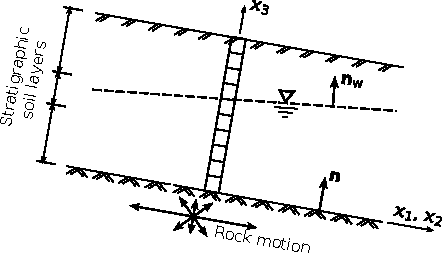
\includegraphics{Figures/Setup}}\quad\quad
    \subfigure{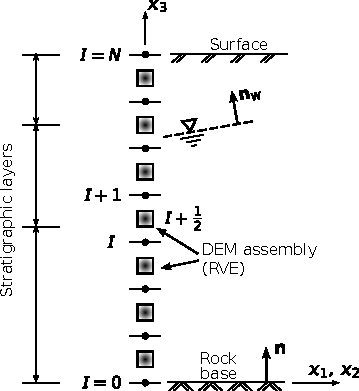
\includegraphics{Figures/Column}}
  }
  \caption{Soil column in Mode~2.  RVEs and Nodes
           are number from the bottom upward.
           The stratigraphic layers are numbered
           from the top downward.}
  \label{fig:column}
\end{figure}
%
Every simulation of wave propagation requires a single
\GFile, which must have a name of the form
\texttt{G}$<$\BaseName$>$\texttt{<suffix>},
as described on
\hyperref[item:BaseName2]{page~\pageref*{item:BaseName2}}.
This file must be placed inside the directory
\BaseName, which must be located in the parent directory
from which \Dempla\ is run.
%
A \GFile\ is a formatted ASCII text file
(\emph{not} a Word file!),
which means that
the input information must be placed within certain rows
and columns (or column ranges).
Sample \GFile s can be 
downloaded from the GitHub site,
and an example of a \GFile\ is shown in
\hyperref[fig:GFile]{Fig.~\ref*{fig:GFile}}.
%
\begin{figure}
	\centering\footnotesize
	GDKS02_bb_B_mu005_f040_A17a.tex
	\caption{An example \textsf{GFile} (column file).
	Because there is only one layer (\texttt{nLayers=1}),
	the file ends with a single line of additional information
	about the one layer.}
	\label{fig:GFile}
\end{figure}
%
%\begin{sidewaysfigure}
%	\centering\footnotesize
%	\begin{verbatim}
Prototype RunFile for the DEM program Oval
       2         : algori   | the algorithm for advancing the particle positions (1 or 2)
       1         : ivers    | whether to include additional lines in this RunFile
       0         : ncownt   | fequency for updating non-periodic boundaries (0)
       0         : iout(2)  | output files with avg. def. and gradients in layers (0 or 1)
       0         : iout(3)  | output files with avg. stresses within layers (0 or 1)
       1         : istart   | type of file defining the initial configuration (1, 2, or 3)
       0         : iend     | type of file to be created at end of the run (0, 1, 2, or 3)
       0         : idef     | reference configuration for reporting deformations (0)
     200         : iupdtm   | max. no. of time steps between linked-list updates
       0         : icirct   | compute and regularly update the particle graph (0 or 1)
       0         : imodel   | model for contact force
       0         : nplatn   | number of additional files with boundary particles
       8         : nloop1   | minimum number of iteration loops when algori=2
     1.00        : kn       | normal stiffness (force/indentation) or G (shear modulus)
     1.00        : kratio   | ratio tangential/normal stiffnesses or Poisson ratio
     0.50        : frict    | coefficient of friction at particle contacts
     0.50        : frictw   | coefficient of friction between particles and wall
     0.          : rho      | the mass density of the particle material
     0.400       : sep      | threshold separation during the near-neighbor searches
     0.05        : pcrit(1) | viscosity coefficient for translational body damping
     0.05        : pcrit(2) | viscosity coefficient for rotational body damping
     0.          : pcrit(3) | viscosity coefficient for contact damping
     0.64        : xseed    | seed for assigning random initial velocities (when motion=1)
     0.          : rmsvel   | rms initial velocity (when motion=1)
     0.          : pdif     | parameter for reducing Jager memory demand (when imodel=6)
     0.          : tmax     | maximum time for the simulation run
     0.          : A_1      | shape factor for conical contact profile (A_1)
     0.          : dt       | time increment
                                                                                         imicro
       ************  Deformation-Stress Path Segments  **********   krotat           iflexc |             iplot
        (100000)   (10000)   (1000)    (100)      (10)      (1)       |            idump  | |ibodyf    ipts2 |
icontr| rate_11 | rate_22 | rate_33 | rate_12 | rate_13 | rate_23 igoal   finalv  ipts |  | | |  defdot  |   |
------|---------|---------|---------|---------|---------|---------|--|-|---------|----|-|--|-|--|------|----|--|
000000      0.        0.        0.         0.       0.        0.   70 0      10.     2 0  0 0  0    0.    0   0
100000      0.     -5.0e-7      0.         0.       0.        0.   70 0   10000.    50 0  0 0  0    0.    0   0
\end{verbatim}

%	\caption{An example \textsf{RunFile} named
%		\texttt{LoadComp} for a biaxial compression test
%		with compression in the $x_{2}$ direction.}
%	\label{}
%\end{sidewaysfigure}
%
I suggest that you use this file as a template for creating your
own \GFile s.
%
\par
A \GFile\ file is arranged in three parts:
\begin{enumerate}
	\item
	a general information section consisting of 26 lines,
	including a comment line
	(see
	\hyperref[sec:Ggeneral]{Section~\ref*{sec:Ggeneral}}).
	The data in these lines have the formats of either
	\texttt{i16} or \texttt{f16.7}, beginning in the
	first column of each line.
	That is, each line contains a single input value 
	at the beginning of the line.
	\item
	eight spacer lines of comments.  These lines are ignored.
	\item
	for each layer, one line of additional information
	is given about the pore fluid and permeability of the layer
	(see
	\hyperref[sec:GFileLayer]{Section~\ref*{sec:GFileLayer}})
	The \GFile\ should include one of these lines per layer.
\end{enumerate}
%
Although the format specifier \texttt{f16.7} is used, Fortran allows
the input data to be in either fixed (\texttt{F}) or
exponential (\texttt{E} or \texttt{D}) formats with any number
of significant digits, \emph{provided that the data fits within the 
first 16 columns of each line}.
%
\subsection{\GFile: General information section}\label{sec:Ggeneral}
%
\subsubsection[\texttt{comment}]{\Var{comment}{\textbackslash}}
The first line of a \GFile\ is ignored.
Put some useful information here.
%
\subsubsection[\texttt{gvers}]{\Var{gvers}{i16}}\label{sec:gvers}
An integer number giving the version of the \GFile.
This variable is included so that current files
will be back-compatible with future versions
of the \Dempla\ code.
The current version is 108,
and \texttt{108} should be place in the second row of the \GFile.
%
\subsubsection[\texttt{nRVEs}]{\Var{nRVEs}{i16}}\label{sec:nRVEs}
The integer number of DEM assemblies (RVEs) in
the soil column
(integer $N$ in \hyperref[fig:column]{Fig.~\ref*{fig:column}}).
In the paper \citep{Kuhn:2021a}, this is the value $N$.
For the simulations in the paper,
\texttt{nRVEs} varied from 17 to 20.
RVEs are numbered from 1 to \texttt{nRVEs}, from the bottom upward.
Nodes are numbered from 0 to \texttt{nRVEs}, from the bottom upward.
\par
The value of \texttt{nRVEs} must not exceed the parameter
\texttt{mrve} in the source code file
\texttt{param-dempla-0.X.X.f}, where ``\texttt{X}'' is the
version number.
The current value is 20.
If you need an \texttt{nRVEs} greater than 20, then
you must change the parameter file and recompile the code
(\hyperref[sec:UnixSystems]{Section~\ref*{sec:UnixSystems}}).
%
\subsubsection[\texttt{nLayers}]{\Var{nLayers}{i16}}\label{sec:nLayers}
The number of stratigraphic layers within the
soil column (\hyperref[fig:column]{Fig.~\ref*{fig:column}}).
Note that one \LFile\ is required for each
stratigraphic layer (see 
\hyperref[sec:LFiles]{Section~\ref*{sec:LFiles}}).
Layers are numbered from 1 to \texttt{nLayers}, from the top downward.
\par
The value of \texttt{nLayers} must not exceed the parameter
\texttt{mLayer} in the source code file
\texttt{param-dempla-0.X.X.f}, where ``\texttt{X}'' is the
version number.
The current value is 100.
If you need an \texttt{nLayers} greater than 100, then
you must change the parameter file and recompile the code
(\hyperref[sec:UnixSystems]{Section~\ref*{sec:UnixSystems}}).
%
\subsubsection[\texttt{iABfile}]{\Var{iABfile}{i16}}\label{sec:iABfile}
When running \Dempla,
the program creates a number of output files:
\AFile s (\hyperref[sec:Afiles]{Section~\ref*{sec:Afiles}}),
\BFile s (\hyperref[sec:Bfiles]{Section~\ref*{sec:Bfiles}}),
\FFile s (\hyperref[sec:ffiles]{Section~\ref*{sec:ffiles}}), and
\ResultsFile s (\hyperref[sec:Results]{Section~\ref*{sec:Results}}).
The \AFile s and \BFile s require more
storage space than other files,
since one \AFile\ and one \BFile\ are created for each RVE.
To conserve disk space,
\texttt{iABfile} is set to \texttt{0},
and \AFile s and \BFile s are not created.
With any other integer value, the files will be created.
%
\subsubsection[\texttt{iPreProcess}]{\Var{iPreProcess}{i16}}\label{sec:iPreProcess}
Before running the \Dempla\ algorithm,
some preprocessing is required:
\begin{itemize}
  \item
    The program must use the information of each stratigraphic
    layer to create the particle contact list and other information for
    the progenitor DEM assembly of the layer.
    The \StartFile\ information about
    each layer is stored as \DFile s for the layers
    (one for each layer),
    since the \StartFile s are likely \DFile s
    (\hyperref[sec:startfileD]{Section~\ref*{sec:startfileD}}).
  \item 
     The program must consolidate the progenitor DEM assemblies
     of the layers to create the RVEs within the layer.
     These DEM assemblies (RVEs) are consolidated to the initial
     conditions of geostatic and hydrostatic pressures at the
     various RVE points.
     These pre-processed assemblies are stored as \CFile s
     for later use at the start of the wave propagation algorithm.
   \item
     The program must determine the stiffness moduli of each
     DEM assembly, so that the wave propagation time step
     can be established (i.e., the time step $\Delta t$
     in \citep{Kuhn:2021a}).
     These moduli are stored as a file in the directory
     \texttt{03\_RVESetup}, so that they can be retrieved later.
\end{itemize}
%
These pre-processing steps can take a lot of time, and they
must only be done once for a given soil column
(for example, once created, the same initial soil column
can be subjected to a number of input motions.
If the pre-processing steps have already been performed,
then a value for \texttt{iPreProcess} of \texttt{0} will
skip the pre-processing of future runs.
Any other integer value of \texttt{iPreProcess} will cause
the pre-processing to be performed.
The pre-processing must be performed at least once.
%
\subsubsection[\texttt{BaseDepth}]{\Var{BaseDepth}{f16.7}}\label{sec:BaseDepth}
The height of the soil column.
%
\subsubsection[\texttt{WaterDepth}]{\Var{WaterDepth}{f16.7}}\label{sec:WaterDepth}
The depth of water below the ground surface.
For dry soil, give a value of \texttt{WaterDepth}
that is greater than \texttt{BaseDepth}.
For a submerged soil column, give a negative value of
\texttt{WaterDepth}.
%
\subsubsection[\texttt{visc\_w}]{\Var{visc\_w}{f16.7}}\label{sec:viscw}
Viscosity of the pore fluid (usually water, 0.0010~Pa$\cdot$s)
for soil below the water table.
This viscosity and the geotechnical hydraulic conductivity
\texttt{k\_geot} are used to calculate the
water permeabilty having units
of $\text{m}^{2}\text{s}^{-1}\text{Pa}^{-1}$
that is used in the Biot equations.
Note that in some of the examples of centrifuge studies,
the water was chemically treated,
so that the viscosity of water.
%
\subsubsection[\texttt{visc\_a}]{\Var{visc\_a}{f16.7}}\label{sec:visca}
Viscodity of the pore fluid
(usually air, about 18.5$\times 10^{-6}$~Pa$\cdot$s)
for soil above the water table.
This viscosity and the geotechnical hydraulic conductivity
\texttt{k\_geot} are used to calculate the
air permeabilty having units
of $\text{m}^{2}\text{s}^{-1}\text{Pa}^{-1}$
that is used in the Biot equations.
%
\subsubsection[\texttt{rho\_w}]{\Var{rho\_w}{f16.7}}\label{sec:rhow}
Density of the pore fluid
(usually water, 998~kg/m\textsuperscript{3})
for soil below the water table.
%
\subsubsection[\texttt{rho\_a}]{\Var{rho\_a}{f16.7}}\label{sec:rhoa}
Density of the pore fluid
(usually air, about 1.18~kg/m\textsuperscript{3})
for soil above the water table.
%
\subsubsection[\texttt{grav}]{\Var{grav}{f16.7}}\label{sec:grav}
Acceleration of gravity (about 9.807~m/s\textsuperscript{2}).
Note that in some of the examples of centrifuge studies,
the acceleration is greater than that of gravity.
%
\subsubsection[\texttt{centrifuge}]{\Var{centrifuge}{f16.7}}\label{sec:centrifuge}
This value is usually 1.0.
However, in centrifuge studies, the mass of the centrifuge
box must be included with the soil mass.
In this case, the input \texttt{centrifuge} is multiplied
by the soil density to account for the box mass.
%
\subsubsection[\texttt{ddef\_target}]{\Var{ddef\_target}{f16.7}}\label{sec:ddeftarget}
When running the wave propagation algorithm,
time is advanced in increments $\Delta t$ (see \citep{Kuhn:2021a}),
and strains within the DEM assemblies are advanced
by an increment $\Delta \varepsilon$ during $\Delta t$.
However, when running the DEM algorithm for each RVE,
the increment $\Delta \varepsilon$ can be achieved in
several DEM time steps,
so that DEM strain is advanced in smaller increments.
These smaller strain increments may be required to maintain
stable and quasi-static conditions when running the DEM
algorithm.
The input \texttt{ddef\_target} gives the maximum DEM
strain increment, so that the simulations remain stable.
What is a suitable value of \texttt{ddef\_target}?
For typical geostatic stresses,
a value between $1\times 10^{-7}$ and $2\times 10^{-6}$
seems to maintain stable simulations
and minimal viscous dissipation,
while reducing run-times.
%
\subsubsection[\texttt{nDempla\_out}]{\Var{nDempla\_out}{i16}}\label{sec:nDemplaout}
The results of a \Dempla\ simulation are given as
output in various \ResultsFile s.
The integer input \texttt{nDempla\_out} gives the frequency
of output in these files.
A value of 1 means that the results of every $\Delta t$
step is written to the \ResultsFile s, a value of 3 means
that the results are written for every third $\Delta t$.
%
\subsubsection[\texttt{nDEM\_out}]{\Var{nDEM\_out}{i16}}\label{sec:nDEMout}
Every time step $\Delta t$ of the \Dempla\ wave propagation
algorithm can involve several DEM time steps.
The integer input \texttt{nDEM\_out} gives the frequency of
reporting the DEM output in the \AFile s and \BFile s.
%
\subsubsection[\texttt{C\_factor}]{\Var{C\_factor}{f16.7}}\label{sec:Cfactor}
Because the dynamic problem solves a wave equation, 
increment $\Delta t$ must be sufficiently
small so that the solution does not outpace the wave equation's
characteristic velocities.
The Courant--Friedrichs-Lewy (CFL) condition requires
the Courant number, $C=c\Delta t/\Delta x$, is less than 1,
where $c$ is the characteristic wave speed.
After initial consolidation but before shaking,
various moduli $Q$ are measured with
small strain-probes so that the corresponding wave
speeds can be estimated.
The moduli include the shear moduli in the $x_{1}$ and $x_{2}$
directions, the drained uniaxial confined compression modulus,
and the undrained
(Biot's closed system)
uniaxial confined compression modulus.
The largest of these moduli among all RVEs
is used to estimate the fastest (local) wave speed $\sqrt{Q/\rho}$,
which is used to compute the increment $\Delta t$
for all RVEs.
\par
Within the \Dempla\ code, a base Courant number of 0.75
is applied to $\Delta x / \sqrt{Q/\rho}$ to compute $\Delta t$,
which is found to achieve marginal stability of the simulation.
An input \texttt{C\_factor} less than 1 reduces $\Delta t$ below
the base value
and can provide more stable simulations.
A value of 0.5 is used in most of the example calculations.
%
\subsubsection[\texttt{Direct\_soil}]{\Var{Direct\_soil}{f16.7}}
The two input values \texttt{Direct\_soil} and \texttt{Dip\_soil}
give the direction and amount of slope of the ground surface
(the complementary values
\texttt{Direct\_water} and \texttt{Dip\_water} give the
direction and amount of slope of the water table).
The two values define the direction $\mathbf{n}$ in
\hyperref[fig:column]{Fig.~\ref*{fig:column}}.
The input \texttt{Direct\_soil} is
the direction (in degrees) of the (downward) slope of the soil
surface (and of the rock base), measured coun\-ter-clock\-wise
from the $x_{1}$ direction (see \citep{Kuhn:2021a}).
%
\subsubsection[\texttt{Dip\_soil}]{\Var{Dip\_soil}{f16.7}}%
\label{sec:Dipsoil}
The downward slope (in degrees) of the soil surface
(and of the rock base).
%
\subsubsection[\texttt{Direct\_water}]{\Var{Direct\_water}{f16.7}}
The two input values \texttt{Direct\_water} and \texttt{Dip\_water}
give the direction and amount of slope of the water table.
The input \texttt{Direct\_water} is
the direction (in degrees) of the (downward) slope of the water
surface, measured coun\-ter-clock\-wise
from the $x_{1}$ direction (see \citep{Kuhn:2021a}).
The two values define the direction $\mathbf{n}_{\text{w}}$
in \hyperref[fig:column]{Fig.~\ref*{fig:column}}.
%
\subsubsection[\texttt{Dip\_water}]{\Var{Dip\_water}{f16.7}}
The downward slope (in degrees) of the water table.
Note that when the water table is above the soil surface
(i.e., the surface is submerged), the water slope must be zero.
%
\subsubsection[\texttt{nTiltSteps}]{\Var{nTiltSteps}{f16.7}}
When the ground surface is sloping,
the DEM assemblies must be slowly sheared so that the
(sloping) geostatic condition is attained.
The input \texttt{nTiltSteps} gives the number of
DEM time steps that are used to apply the geostatic
shear stress.
%
\subsubsection[\texttt{nTiltEquil}]{\Var{nTiltEquil}{f16.7}}
When the ground surface is sloping,
the DEM assemblies must be slowly sheared so that the
(sloping) geostatic condition is attained.
After the assemblies are sheared,
the input number \texttt{nTiltEquil} of DEM time steps
is used for the assemblies to equilibrate.
%
\subsubsection[\texttt{t\_PostShake}]{\Var{t\_PostShake}{f16.7}}
The input values of \texttt{t\_PostShake} and \texttt{t\_Setl}
specify actions after the shaking is finished
(i.e., after the full input base motion in
the \MotionFile\ has complete, see
\hyperref[sec:MFiles]{Section~\ref*{sec:MFiles}}).
After shaking,
the input value of \texttt{t\_PostShake} gives the
duration (time) of a quiescent period in which the
dynamic algorithm of \Dempla is implemented with zero
base motion. 
%
\subsubsection[\texttt{t\_Setl}]{\Var{t\_Setl}{f16.7}}
After the shaking is finished and after the quiescent
period of duration \texttt{t\_PostShake} is finished,
the input \texttt{t\_Setl} gives the duration (time) in
which the consolidation algorithm is conducted
(see \citep{Kuhn:2021a} for the distinction of shaking
and consolidation algorithms).
%
%
\subsection{\GFile: Layer options section}\label{sec:GFileLayer}
The final section of a \GFile gives some additional
information about each layer (for example, the layer's
permeability).
This part of the \GFile must have one line per stratigraphic
layer (i.e., the number of layers \texttt{nLayers},
\hyperref[sec:nLayers]{Section~\ref*{sec:nLayers}}).
The lines are arranged sequentially, with each
line specifying a single layer,
starting with the top layer and ending with the bottom layer.
Each line contains 4 fields, arranged and formatted as follows:\\[-2ex]
%
\begin{verbatim}
	format(i4,1x,    lSat
	f9.6,1x,         xSat
	f9.6,1x,         k_geot
	i4,1x,           iCap
	f9.6)            xCap
\end{verbatim}
\rule{0ex}{3ex}%
Note that the input fields are separated with the blank character
(\texttt{1x}) and are arranged horizontally \emph{on a single line}.
Each line defines a single stratigraphic layer.
Each layer must also have its own \LFile.
%
\subsubsection[\texttt{lSat}]{\Var{lSat}{i4, 1x}}\label{sec:lSat}
The input values \texttt{lSat} and \texttt{xSat} only apply
when the layer is initially saturated (i.e., with no gas bubbles)
and the poromechanic model \texttt{iporo=3} is being used
(see \hyperref[sec:iporo]{Section~\ref*{sec:iporo}}).
In this situation,
the values \texttt{lSat} and \texttt{xSat} allow you specify
the amount of dissolved gas in the pore water.
The amount of dissolved gas can be set with the
value of \texttt{p\_wcav} in the 
\RunFile\ (see \hyperref[sec:pwcav]{Section~\ref*{sec:pwcav}}),
but with \texttt{lSat} and \texttt{xSat}, you can change
these values at the start of the wave propagation algorithm.
Th input \texttt{lSat} tells the program
whether to use a special saturation condition for the layer,
over-riding \texttt{p\_wcav}.
%
\begin{Options}
	\item[lSat=0]
      No special treatment, and the value of \texttt{xSat}
      is ignored.
      When \texttt{iporo=3}, use the values of \texttt{S\_o},
      \texttt{p\_o}, and \texttt{p\_wcav} in the \RunFile\ of
      this layer
      (see Sections~\ref{sec:So}, \ref{sec:po}, and \ref{sec:pwcav}).
      The \RunFile\ for the layer 
      should be located in the \texttt{RunFile}s
      sub-directory 
      (\hyperref[item:RunFileDir]{page~\pageref*{item:RunFileDir}}),
      and the name of the file
      should be given in the \LFile\ for the layer
      (\hyperref[sec:RunFileLayer]{Section~\ref*{sec:RunFileLayer}}).
    \item[lSat=1]
      When \texttt{iporo=3} and \texttt{S\_o}=1.0,
      then the pore water pressure \texttt{p\_o} will be reset to the
      hydrostatic pressure at the end of consolidation,
      and \texttt{p\_wcav} (i.e., the relative pressure at which
      disolved gas will cavitate and bubbles will form,
      as in \hyperref[sec:pwcav]{Section~\ref*{sec:pwcav}})
      will be reset to this water pressure minus the value of
      \texttt{xSat} (elsewhere in the code, pressure \texttt{u\_wcav}),
      which should have a value greater than 0.
      When \texttt{iporo=3} but \texttt{S\_o} $<$ 1.0, 
      then \texttt{xSat} is ignored and the program uses
      the values of \texttt{S\_o}, \texttt{p\_o},
      and \texttt{p\_wcav} in the \RunFile.
    \item[lSat=2]
      When \texttt{iporo=3} and \texttt{S\_o=1.0},
      then \texttt{p\_o} will be reset to the
      water pressure at the end of consolidation,
      and \texttt{p\_wcav}
      (elsewhere in the code, pressure \texttt{u\_wcav})
      will be reset to this water pressure
      times the value of \texttt{xSat},
      which should have a value between 0 and 1.
      When \texttt{iporo=3} but \texttt{S\_o} $<$ 1.0,
      then use the values of
      \texttt{S\_o}, \texttt{p\_o}, and \texttt{p\_wcav}
      in the \RunFile\ of this 
      layer in the \RunFile s sub-directory.
      Note that cavitation is disallowed unless the following values
      are included in the layer \RunFile:
      \texttt{iporo=3}, \texttt{S\_o}=1.0,
      \texttt{N\_o} is non-zero
      (\hyperref[sec:No]{Section~\ref*{sec:No}}),
      and \texttt{Hcc} is non-zero
      (\hyperref[sec:Hcc]{Section~\ref*{sec:Hcc}}).
\end{Options}
%
%
\subsubsection[\texttt{xSat}]{\Var{xSat}{f9.6, 1x}}\label{sec:xSat}
When \texttt{lSat} is 1 or 2 and \texttt{S\_o} = 1,
the value of \texttt{xSat} is used for 
adjusting \texttt{p\_wcav}
(elsewhere in the code, pressure \texttt{u\_wcav}),
which is the value of the water pressure, 
below which cavitation occurs.
%
\begin{Options}
  \item[lSat=0]
    When \texttt{lSat}=0,
    no special treatment, and \texttt{xSat} is ignored.
  \item[lSat=1]
    When \texttt{lSat=1},
    and \texttt{iporo=3} and \texttt{S\_o}=1.0,
    then \texttt{p\_o} will be reset to the hydrostatic
    water pressure at the end of consolidation,
    and \texttt{p\_wcav}
    will be reset to the hydrostatic pressure
    minus the value of \texttt{xSat}
    (which should be greater than 0).
    When \texttt{iporo=3} but \texttt{S\_o}$<$1.0, then
    \Dempla\ will ignore \texttt{xSat} 
    and use the values of \texttt{S\_o},
    \texttt{p\_o}, and \texttt{p\_wcav} in the
    \RunFile\ of the layer.
    For example, when
    \texttt{lSat}=1, \texttt{iporo}=3,
    and \texttt{S\_o}=1, and \texttt{xSat} = 10,
    then the pore water is under-saturated with air,
    and cavitation will occur when the water pressure in the
    RVE assembly is reduced to 10Pa below the hydrostatic pressure.
  \item[lSat=2]
    When \texttt{lSat=2},
    and \texttt{iporo=3} and \texttt{S\_o}=1.0,
    then \texttt{p\_o} will be reset to the hydrostatic
    water pressure at the end of consolidation,
    and \texttt{p\_wcav}
    will be set to the hydrostatic pressure
    times the value of \texttt{xSat},
    which should be a value between 0 and 1.
    When \texttt{iporo=3} but \texttt{S\_o}$<$1.0, then
    \Dempla\ will ignore \texttt{xSat} 
    and use the values of \texttt{S\_o},
    \texttt{p\_o}, and \texttt{p\_wcav} in the
    \RunFile\ of the layer.
    For example, when
    \texttt{lSat}=1, \texttt{iporo}=3,
    and \texttt{S\_o}=2, and \texttt{xSat} = 0.90,
    then the pore water is under-saturated with air,
    and cavitation will occur when the water pressure in the
    RVE assembly is reduced to 90\% of the (absolute)
    hydrostatic pressure.
\end{Options}
%
%
\subsubsection[\texttt{k\_geot}]{\Var{k\_geot}{f9.6, 1x}}\label{sec:k_geot}
The value of hydraulic conductivity
for the stratigraphic layer.
This is the standard geotechnical permeability with units
of m/s.
%
%
\subsubsection[\texttt{iCap}]{\Var{iCap}{i4, 1x}}\label{sec:iCap}
The integer \texttt{iCap} specifies whether to cap
the pore water pressure (relative to the
hydrostatic pressure), perhaps to prevent pressure surges 
due to bubble collapse.
\begin{Options}
  \item[iCap=0]
    No cap is placed on the pore water pressure,
    and \texttt{xCap} is ignored.
  \item[iCap=1]
    The pore water pressure is capped to a pressure of \texttt{xCap}
    above the hydrostatic pressure.
\end{Options}
%
%
\subsubsection[\texttt{xCap}]{\Var{xCap}{f9.6, 1x}}\label{sec:xCap}
When \texttt{iCap}=1, then the
pore water pressure is capped to a pressure of \texttt{xCap}
above the hydrostatic pressure.
%
%
\section{LFiles (Layer files)}\label{sec:LFiles}
These files give basic information about stratigraphic
soil layers.
If you are running \Dempla\ in Mode~1,
you can skip this section --- \LFile s are not needed.
Each layer requires a corresponding \LFile.
As explain in
\hyperref[sec:Lfiles0]{item~3} on
\hyperref[sec:Lfiles0]{page~\pageref*{sec:Lfiles0}},
the \LFile s must have a specific name and must be located
in a specific directory.The \LayerFile\ must have the name
\texttt{L<XXXX>\_}\BaseName.
The name begins with letter ``\texttt{L}'',
followed by a 4-digit number
(beginning with \texttt{0001} for the top soil layer,
and increasing with \texttt{0002}, \texttt{0003}, etc.
to the bottom layer).
The number is followed by an underscore ``\texttt{\_}''
and the \BaseName.
%
An \LFile\ is an ASCII text formatted input file
(\emph{not} a Word file!),
which means that
the input information must be placed within certain rows
and columns (or column ranges).
Sample \LFile s can be 
downloaded from the GitHub site,
and an example of an \LFile\ is shown in
\hyperref[fig:LFile]{Fig.~\ref*{fig:LFile}}.
%
%
\begin{figure}
	\centering\footnotesize
	L0001_DKS02_bb_B_mu005_f040_A17.tex
	\caption{An example \textsf{LFile} (layer file).
	Among other information, the file gives the name
    of the \RunFile\ for the layer and the \StartFile\ of
    the initial particle arrangement.}
	\label{fig:LFile}
\end{figure}
%
%\begin{sidewaysfigure}
%	\centering\footnotesize
%	\begin{verbatim}
Prototype RunFile for the DEM program Oval
       2         : algori   | the algorithm for advancing the particle positions (1 or 2)
       1         : ivers    | whether to include additional lines in this RunFile
       0         : ncownt   | fequency for updating non-periodic boundaries (0)
       0         : iout(2)  | output files with avg. def. and gradients in layers (0 or 1)
       0         : iout(3)  | output files with avg. stresses within layers (0 or 1)
       1         : istart   | type of file defining the initial configuration (1, 2, or 3)
       0         : iend     | type of file to be created at end of the run (0, 1, 2, or 3)
       0         : idef     | reference configuration for reporting deformations (0)
     200         : iupdtm   | max. no. of time steps between linked-list updates
       0         : icirct   | compute and regularly update the particle graph (0 or 1)
       0         : imodel   | model for contact force
       0         : nplatn   | number of additional files with boundary particles
       8         : nloop1   | minimum number of iteration loops when algori=2
     1.00        : kn       | normal stiffness (force/indentation) or G (shear modulus)
     1.00        : kratio   | ratio tangential/normal stiffnesses or Poisson ratio
     0.50        : frict    | coefficient of friction at particle contacts
     0.50        : frictw   | coefficient of friction between particles and wall
     0.          : rho      | the mass density of the particle material
     0.400       : sep      | threshold separation during the near-neighbor searches
     0.05        : pcrit(1) | viscosity coefficient for translational body damping
     0.05        : pcrit(2) | viscosity coefficient for rotational body damping
     0.          : pcrit(3) | viscosity coefficient for contact damping
     0.64        : xseed    | seed for assigning random initial velocities (when motion=1)
     0.          : rmsvel   | rms initial velocity (when motion=1)
     0.          : pdif     | parameter for reducing Jager memory demand (when imodel=6)
     0.          : tmax     | maximum time for the simulation run
     0.          : A_1      | shape factor for conical contact profile (A_1)
     0.          : dt       | time increment
                                                                                         imicro
       ************  Deformation-Stress Path Segments  **********   krotat           iflexc |             iplot
        (100000)   (10000)   (1000)    (100)      (10)      (1)       |            idump  | |ibodyf    ipts2 |
icontr| rate_11 | rate_22 | rate_33 | rate_12 | rate_13 | rate_23 igoal   finalv  ipts |  | | |  defdot  |   |
------|---------|---------|---------|---------|---------|---------|--|-|---------|----|-|--|-|--|------|----|--|
000000      0.        0.        0.         0.       0.        0.   70 0      10.     2 0  0 0  0    0.    0   0
100000      0.     -5.0e-7      0.         0.       0.        0.   70 0   10000.    50 0  0 0  0    0.    0   0
\end{verbatim}

%	\caption{An example \textsf{RunFile} named
%		\texttt{LoadComp} for a biaxial compression test
%		with compression in the $x_{2}$ direction.}
%	\label{}
%\end{sidewaysfigure}
%
I suggest that you use this file as a template for creating your
own \LFile s.
%
\par
An \LFile\ contains 8 lines, described in the eight subsections
below.
Except for the first line, the beginning of each line contains
the value a particular \Dempla\ input variable.
The lines give the value of the following variables,
with the corresponding format.
%
%\subsection[\texttt{comment}]{\Var{comment}{\textbackslash}}
%
\subsection[\texttt{comment}]{\Var{comment}{\textbackslash}}
The first line of a \LFile\ is ignored.
Put some useful information here.
%
\subsection[\texttt{lvers}]{\Var{lvers}{i16}}%
\label{sec:lvers}
An integer number giving the version of the \GFile.
This variable is included so that current files
will be back-compatible with future versions
of the \Dempla\ code.
The current version is 102,
and \texttt{102} should be place in the second row of the \LFile.
%
\subsection[\texttt{Isotropic}]{\Var{Isotropic}{i16}}%
\label{sec:Isotropic}
When \Dempla\ does the preprocessing to prepare the soil
column,
the RVEs in each layer are consolidated to the
geostatic and hydrostatic conditions of the RVE levels.
Each layer begins as a single progenitor DEM assembly
(i.e., a single \DFile),
which is consolidated to the particular conditions
of each RVE within the layer.
This initial consolidation can be performed isotropically
or anisotropically.
%
\begin{Options}
  \item[Isotropic=0,1]
    A value of 0 or 1 means that
    the layer will be consolidated isotropically by 
    increasing (or decreasing) the normal stresses
    $\sigma_{11}$, $\sigma_{22}$, and $\sigma_{33}$
    at equal rates, until the target geostatic
    conditions are attained.
    Note that the shearing stresses
    $\sigma_{13}$ and $\sigma_{23}$ will also
    be increased (or decreased), in the case of
    a sloping ground surface or a sloping water table.
  \item[Isotropic=2]
    The layer will be consolidated anisotropically by
    maintaining zero strain in the lateral directions,
    while 
    increasing (or decreasing) the normal stress
    $\sigma_{33}$.
    Note that the shearing stresses
    $\sigma_{13}$ and $\sigma_{23}$ will also
    be increased (or decreased), in the case of
    a sloping ground surface or a sloping water table.
\end{Options}
%
\subsection[\texttt{LayerThickness}]{\Var{LayerThickness}{f16.7}}%
\label{sec:LayerThickness}
The thickness of the stratigraphic soil layer.
The sum of the thicknesses of all soil layers in the soil column
must exceed the height of the column.
%
\subsection[\texttt{VoidRatio}]{\Var{VoidRatio}{f16.7}}%
\label{sec:VoidRatio}
The presumed initial void ratio of the stratigraphic soil
layer.
This void ratio might be the same as the void ratio of the
DEM assembly,
but the presumed void ratio will be used for computing
the soil density.
The presumed void ratio will be adjusted while running
the \Dempla\ algorithm, in accordance with the volume
change of the DEM assemblies.
%
\subsection[\texttt{G\_s}]{\Var{G\_s}{f16.7}}%
\label{sec:G_s}
The specific gravity of the soil grains,
which is used to find the soil density
(note that the density of water is given in the
\GFile, 
\hyperref[sec:rhow]{Section~\ref*{sec:rhow}}).
%
\subsection[\texttt{RunFileLayer}]{\Var{RunFileLayer}{a400}}%
\label{sec:RunFileLayer}
The name of the \RunFile\ for the layer.
This \RunFile\ will be used to prepare the DEM assemblies
for the RVEs:
the contact model and properties,
the poromechanic model and properties,
and other run variables.
The name of \texttt{RunFileLayer} file must conform to Linux
naming conventions of files, case-sensitive with no spaces.
The file with this name must be located within the
\texttt{RunFiles} folder within the base folder for the
simulation.
The contents and format
of \RunFile s are described in
\hyperref[sec:RunFile]{Section~\ref*{sec:RunFile}}.
%
\subsection[\texttt{StartFileLayer}]{\Var{StartFileLayer}{a400}}%
\label{sec:StartFileLayer}
The name of the \StartFile\ for the layer.
This \StartFile\ is a \DFile\ that
contains information about the assembly
of particles:
number of particles, shape category of the particles,
sizes of particle, and locations and orientations of particles.
The name of \texttt{StartFileLayer} must conform to Linux
conventions, case-sensitive with no spaces.
The file with this name must be located within the
\texttt{StartFiles} folder within the base directory
from which the
simulation is run.
%
\par
Although the \Oval\ engine in \Dempla\ accommodates
several different boundary types
(\hyperref[sec:Boundaries]{Section~\ref*{sec:Boundaries}}),
only D-type \StartFile s (i.e., \DFile s)
with periodic boundaries
are currently permitted with Mode~2 (wave propagation)
analyses.
Mode~2 analyses can only be conducted in three dimensions,
and only 3-d assemblies are permitted.
The contents and format
of D-type \StartFile s are described
in \hyperref[sec:startfileD]{Section~\ref*{sec:startfileD}}.
When running \Dempla, the deformation gradient
is described by an upper-triangular matrix
(\hyperref[sec:icontr]{Section~\ref*{sec:icontr}}).
The initial deformation gradient is the $3\times 3$ identity matrix.
%
%
\section{MFiles (Motion files)}\label{sec:MFiles}
An \MFile\ or \MotionFile\ gives the displacement
history of the soil column's base (i.e. rock, or at the
depth at which a otion was actually recorded).
\MFile s are only used in Mode~2 (wave-propagation)
DEM analyses.
\MFile s are not used with Mode~1 (single-assembly)
DEM analyses.
Displacements are given in the two lateral directions
$x_1$ and $x_2$ (parallel to the ground and rock surfaces)
and the direction $x_3$ that is perpendicular
to the ground and rock surfaces (vertical for non-sloping ground).
The displacements must begin with zero displacements in all
three directions.
I recommend that the displacement history end 
(i.e. the last line in the \MFile) such that the
final velocity is zero or nearly zero.
The first line of the file gives the time increment between
displacement steps (this time increment will likely be different
than the $\Delta t$ of the wave propagation algorithm).
The first line is following by lines of the displacement history
(the number of lines are limited by the parameter \texttt{mRock}
in the source code file \texttt{param-dempla-X.X.XX.f})
The current value is 50,000.
%
\subsection[\texttt{dtRock}]{\Var{dtRock}{*}}
The time increment (seconds) between rock displacement values.
Use double precision format (e.g. \texttt{5.000000d-04}).
This value will likely differ from $\Delta t$
in the wave propagation algorithm
(see \citep{Kuhn:2021a}).
%
\subsection[\texttt{xRock(1:3,*)}]{\Var{dtRock}{xRock(1,i), xRock(2,i), xRock(3,i)}}
Rock displacements (meters) in the three directions.
Use three double precision values (e.g. \texttt{5.000000d-04}),
separated by zeros.
The $x_{3}$ direction is perpendicular to the
(possibly sloping) rock base.
%
%
\section{Boundary Types}\label{sec:Boundaries}
\Dempla\ (and before it, \Oval)
is primarily intended for element studies of using rectangular (2D) and
box (3D) assemblies of particles.
During a simulation, the boundaries (sides) are moved to produce
prescribed rates of strain or rates of stress, as described in
\hyperref[sec:runfile2]{Section~\ref*{sec:runfile2}}.
The boundaries themselves can be of several types.
%
\subsection{Periodic boundaries}\label{sec:Periodic}
The default boundaries are periodic.
These are the easiest boundaries to use, 
and they can be used with either dense or sparse assemblies.
Moreover, some of the other types of boundaries are created by starting
with an assembly having periodic boundaries and then replacing the
periodic boundaries with the another boundary type.
%
\par
For Mode~2 (wave propagation) analyses,
only three-dimensional assemblies
with periodic boundaries are permitted.
%
\subsection{Tight-fitting particle boundaries}\label{sec:TightFitting}
This type of boundary can only be created with 2D assemblies,
and it is created by beginning with a non-sparse (at least, moderately
dense) assembly having periodic boundaries.
The process of creating a tight-fitting particle boundary involves
finding the particle graph of the assembly (i.e., finding the
topological arrangement of the contacts) and then identifying the string
of contacting particles that surround the assembly.
These particles become the boundary particles, which will fit tightly
against (i.e., will be in contact with) the interior particles.
After the periodic boundaries are ``broken'' and replaced with
tight-fitting boundaries, the boundary particles will not likely be
in equilibrium, so a period of several hundred time steps should be
included to allow the assembly to equilibrate with its new boundaries.
Once periodic boundaries are replaced with tight-fitting particle boundaries,
the periodic boundaries can not be retrieved.
Tight-fitting boundaries can be placed on the left and right sides (with
periodic boundaries remaining top and bottom), on the the top and bottom
(with periodic boundaries remaining left and right), or on all four sides
of the assembly.  The intended combination of boundaries is specified
with the \texttt{iflexc} input variable
(\hyperref[sec:iflexc]{Section~\ref*{sec:iflexc}}).
\par
Several types of stress or strain control are available with tight-fitting
boundaries:
\begin{itemize}
\item
Stress control (\texttt{iflexc = x1, 1x,} or \texttt{11}).
The stress (actually, the stress rate) can be controlled with
the \texttt{icontr=1} and \texttt{defrat} at the desired rate
(\hyperref[sec:icontr]{Section~\ref*{sec:icontr}} 
and \hyperref[sec:icontr]{Section~\ref*{sec:icontr}}).
For example, if tight-fitting boundaries are created on the left and
right sides, the stress $\sigma_{11}$ is applied against the two sides,
and the rate of this stress can be controlled.
In this same example, the other stress components ($\sigma_{12}$,
$\sigma_{21}$, and $\sigma_{22}$) are also applied on the left and right
sides, but only their original (not current) values are applied 
(those stresses present when the tight-fitting boundary was created).
This approach prevents ``hydro-fracturing'' of the side boundaries if
the assembly is being compressed vertically.
Stress-controlled tight-fitting boundaries approximate the membrane-type
conditions that are commonly used in soil testing.
The boundary stress is applied to imaginary boundary element: 
the branch vectors that connect the centers of the boundary particles.
\item
Displacement control with free rotation 
(\texttt{iflexc = x2, 2x,} or \texttt{22}).
The particles along a tight-boundary are constrained to translate at
a rate in accord with the prescribed strain rates
(\hyperref[sec:icontr]{Section~\ref*{sec:icontr}}
and \hyperref[sec:defrat]{Section~\ref*{sec:defrat}}).
The boundary particles are allowed to rotate.
Boundary forces are applied at the centers of the boundary particles.
\item
Displacement control with free rotation
(\texttt{iflexc = x3, 3x,} or \texttt{33}).
The particles along a tight-boundary are constrained to translate at
a rate in accord with the prescribed strain rates
(\hyperref[sec:icontr]{Section~\ref*{sec:icontr}}
and \hyperref[sec:defrat]{Section~\ref*{sec:defrat}}).
The boundary particles constrained to rotate in accord with the
prescribed rotation rate (the Eulerian rate that corresponds
to $\frac{1}{2}F_{12}$ in
\hyperref[sec:icontr]{Section~\ref*{sec:icontr}}.
Boundary forces are applied at the centers of the boundary particles.
\item
Displacement control with friction and free rotation
(\texttt{iflexc = x4, 4x,} or \texttt{44}).
Suppose that tight-fitting boundaries have been created on the left
and right sides, and periodic boundaries remain on the top and bottom
(\texttt{iflexc = 40}).
With this type of control, particles along the left and right sides
are constrained to translate horizontally at
a rate in accord with the prescribed horizontal strain rates $F_{11}$
and $F_{12}$
(\hyperref[sec:icontr]{Section~\ref*{sec:icontr}}
and \hyperref[sec:defrat]{Section~\ref*{sec:defrat}}).
The side particles are free to translate vertically, but only if they
overcome the side friction coefficient prescribed by 
\texttt{frictw}
(\hyperref[sec:frictw]{Section~\ref*{sec:frictw}}).
The boundary particles are allowed to rotate.
Boundary forces are applied at the centers of the boundary particles.
\item
Displacement control with friction and free rotation
(\texttt{iflexc = x5, 5x,} or \texttt{55}).
Suppose that tight-fitting boundaries have been created on the left
and right sides, and periodic boundaries remain on the top and bottom
(\texttt{iflexc = 40}).
With this type of control, particles along the left and right sides
are constrained to translate horizontally at
a rate in accord with the prescribed horizontal strain rates $F_{11}$
and $F_{12}$
(\hyperref[sec:icontr]{Section~\ref*{sec:icontr}}
and \hyperref[sec:defrat]{Section~\ref*{sec:defrat}}).
The side particles are free to translate vertically, but only if they
overcome the side friction coefficient prescribed by
\texttt{frictw}
(\hyperref[sec:frictw]{Section~\ref*{sec:frictw}}).
The boundary particles constrained to rotate in accord with the
prescribed rotation rate (the Eulerian rate that corresponds
to $\frac{1}{2}F_{12}$ in
\hyperref[sec:icontr]{Section~\ref*{sec:icontr}}).
Boundary forces are applied at the centers of the boundary particles.
\end{itemize}
%
\subsection{Rigid-flat boundaries}\label{sec:RigidFlat}
This type of boundary can be created with either 2D or 3D assemblies.
The boundary is produced by giving an input value for 
\texttt{iflexc} of \texttt{9}, \texttt{90}, or \texttt{99}
in the first line of the deformation-stress path section
of a \RunFile\ (see 
\hyperref[sec:iflexc]{Section~\ref*{sec:iflexc}}).
A pair of rigid-flat boundaries (one each on opposite sides of
the assembly) can coexist with periodic boundaries on the other sides.
The size of the assembly (the box dimensions) are input
with the dimensions \texttt{xcell} 
(\hyperref[sec:xcell11]{Section~\ref*{sec:xcell11}}
and \hyperref[sec:xcell12]{Section~\ref*{sec:xcell12}}).
Unlike with tight-fitting boundaries
(\hyperref[sec:TightFitting]{Section~\ref*{sec:TightFitting}}),
particles interact with rigid-flat boundaries at the particle
surfaces, instead of at the particle centers.
Stresses and strains can be controlled with rigid-flat boundaries,
just as with other types of boundaries
(\hyperref[sec:icontr]{Section~\ref*{sec:icontr}}
through \hyperref[sec:finalv]{Section~\ref*{sec:finalv}}).
%
\subsection{External-particle boundaries}\label{sec:ExternalParticles}
These boundaries are created by surrounding the assembly with
a set of external particles, which confine the interior particles.
This type of boundary can be created with either 2D or 3D assemblies.
The boundary is produced by giving an input value of greater than one
to the integer \texttt{nplatn}
(\hyperref[sec:nplatn]{Section~\ref*{sec:nplatn}}).
For example, if \texttt{nplatn=4}, then you will be queried to
give the names of four files that provide information about
each of the four sets of
boundary particles---their positions, radii, etc.---as described below.
Stresses and strains can be controlled with rigid-flat boundaries,
just as with other types of boundaries
(\hyperref[sec:icontr]{Section~\ref*{sec:icontr}}
through \hyperref[sec:finalv]{Section~\ref*{sec:finalv}}).
Note that the boundary particles can only be circles (2D) or spheres (3D).
\par
A file that provides information about a set of boundary
particles contains four lines that give general information about
the particles followed lines that provide information on each particle.
The content of each line is described in the following
subsections (Fortran free format is used, with integer or double precision
type corresponding to the leading letter of the variable name).
%
\subsubsection[\texttt{ipvers}]{\texttt{ipvers}}%
\label{sec:pb1}
Set this value to 1.  It gives a version number for the file, in the
event that future changes are made to the format of these files.
%
%
\subsubsection[\texttt{ixfix(1)}]{\texttt{ixfix(1),ixfix(2),ixfix(3),ithfix(1),ithfix(2),ithfix(3)}}%
\label{sec:pb2}
The manner in which the boundary particles are constrained in their motions.
Values of either \texttt{0} or \texttt{1} (unconstrained or constrained,
respectively) are assigned to the three directions of translation,
(\texttt{ixfix}), and the three directions of rotation, (\texttt{ithfix}).
Note that when translation is constrained in a particular direction, then
the boundary particle move in accord with the prescribed
deformation rate $F_{ij}$
(\hyperref[sec:icontr]{Section~\ref*{sec:icontr}}).
%
\subsubsection[\texttt{idirec}]{\texttt{idirec}}%
\label{sec:pb3}
The ``direction'' of the boundary.  For example, if a set of boundary 
particles are one the left (i.e., $x_{1}$) side of a 2D assembly, 
then \texttt{idirec} is set to 1.  If a set of boundary
particles are one the top or bottom of a 2D assembly, 
then \texttt{idirec} is set to 2 (i.e., $x_{2}$).
This feature is necessary to enable the control of stress within these
boundaries.
%
\subsubsection[\texttt{nplt}]{\texttt{nplt}}%
\label{sec:pb4}
The number of particles in the boundary file.
%
\subsubsection[\texttt{rad,xp(1)}]{\texttt{rad,xp(1),xp(2),xp(3)}}%
\label{sec:pb5}
The radius and position of a particle center, with one particle per line
of input.
%
\section{\textsf{RunFile}s for \Dempla\ and \Oval}\label{sec:RunFile}
\RunFile s give general information about the conditions
of the DEM analysis.
\RunFile s are required for either Mode~1 (single assembly)
or Mode~2 (wave propagation) analysis.
The ASCII text file is a formatted input file, which means that
the input information must be placed within certain rows
and columns (or column ranges).
Sample \textsf{RunFile}s can be 
downloaded from the web site,
and an example of a \textsf{RunFile} is shown in Figs.~\ref{fig:LoadComp1}
and~\ref{fig:LoadComp2}, which give the upper and lower parts of
the file.
%
\begin{sidewaysfigure}
\centering\footnotesize
\begin{verbatim}
Heading with useful information about this particular simulation
       1         : algori   | the algorithm for advancing the particle positions (1 or 2)
       6         : ivers    | add extra input lines (0)
       0         : ncownt   | fequency for updating non-periodic boundaries (0)
       0         : iout(2)  | output files with avg. def. and gradients in layers (0)
       0         : iout(3)  | output files with avg. stresses within layers (0)
       1         : istart   | type of file defining the initial configuration (1 or 3)
       0         : iend     | type of file to be created at end of the run (0, 1, or 3)
       0         : idef     | reference configuration for reporting deformations (0)
     500         : iupdtm   | max. no. of time steps between linked-list updates
       0         : icirct   | compute and regularly update the particle graph (0)
       9         : imodel   | contact model (linear, Hertz, etc.) (0 1, 5, 6, 7, or 9)
       0         : nplatn   | number of additional D-files with boundary particles (0)
       5         : nloop1   | minimum number of iteration loops when algori=2
       0         : iexact   | don't use the same mass for every particle (0 or 1)
       0         : isub     | number of submerged particles (0)
       1         : idamp    | standard or Potyondy/Cundall damping (0, 1, 2, or 3)
       0         : iheat    | temperature-dependent model (0)
       0         : icoef    | enable changing the friction coefficient during a run (0)
       3         : iporo    | poromechanic fluid model (0, 1, 3, or 4)
       0         : ifree(11)| a free input integer.  Placeholder for future versions
       0         : ifree(12)| a free input integer.  Placeholder for future versions
       0         : ifree(13)| a free input integer.  Placeholder for future versions
       0         : ifree(14)| a free input integer.  Placeholder for future versions
       0         : ifree(15)| a free input integer.  Placeholder for future versions
       0         : ifree(16)| a free input integer.  Placeholder for future versions
       0         : ifree(17)| a free input integer.  Placeholder for future versions
       0         : ifree(18)| a free input integer.  Placeholder for future versions
\end{verbatim}

\caption{An example \textsf{RunFile} -- the upper 28 lines.}
\label{fig:LoadComp1}
\end{sidewaysfigure}
%
\begin{sidewaysfigure}
\centering\footnotesize
\begin{verbatim}
    29.d9        : kn       | normal contact stiffness (force/indentation)
     0.15        : kratio   | ratio of tangential/normal contact stiffnesses
     0.40        : frict    | coefficient of friction at particle contacts
     0.          : frictw   | coefficient of friction between particles and wall
    -1.          : rho      | the mass density of the particle material
     0.250       : sep      | threshold separation during the near-neighbor searches
     0.03        : pcrit(1) | viscosity coefficient for translational body damping
     0.05        : pcrit(2) | viscosity coefficient for rotational body damping
     0.          : pcrit(3) | viscosity coefficient for contact damping
     0.64        : xseed    | seed for assigning random initial velocities (when motion=1)
     0.          : rmsvel   | rms initial velocity (when motion=1)
     0.25        : pdif     | parameter for reducing Jager memory demand (when imodel>=6)
     0.          : tmax     | maximum time for the simulation run
   100.          : A_1      | shape factor for conical or general contact asperity profile
    -1.          : dt       | time increment
     0.          : gravty(1)| gravity in x_1 direction. Depracated. (0.)
     0.          : gravty(2)| gravity in x_2 direction. Depracated. (0.)
     0.          : gravty(3)| gravity in x_3 direction. Depracated. (0.)
     0.          : p_o      | initial fluid pressure of pore liquid relative to atm. pressure
    31.8d9       : K_s      | bulk modulus of grain bodies (when iporo = 1, 3, or 4)
     2.2d9       : K_f      | bulk modulus of pore fluid (when iporo = 1 or 3)
     1.00d0      : S_o      | initial fluid saturation of pore fluid at p_o (iporo=3)
   100.d3        : p_atm    | the reference atmospheric pressure (iporo=3)
     0.          : Hcc      | Henry's coefficient of solubility of pore gas (iporo=3)
    72.75d-3     : gamm     | surface tension of pore bubbles (iporo=3)
     0.0001d0    : D_o      | initial bubble diameter at p_o and S_o (iporo=3)
     2.d13       : N_o      | number/density bubbles per unit initial pore volume(iporo=3)
  2337.d0        : p_vap    | water vapor pressure as abs. pressure (iporo=3)
     0.          : p_wcav   | cavitation pressure relative to atm. pressure (iporo=3)
     0.          : rfree(15)| placeholder
     0.          : rfree(16)| placeholder
     0.          : rfree(17)| placeholder
     0.          : rfree(18)| placeholder
     1.5         : palpha   | alpha power in contact profile (when imodel=9)
                                                                                                   imicro
       ************  Deformation-Stress Path Segments  **********             krotat           iflexc |             iplot
   icontp (100000)   (10000)   (1000)    (100)      (10)      (1)                 |            idump  | |ibodyf    ipts2 |
icontr |  rate_11 | rate_22 | rate_33 | rate_12 | rate_13 | rate_23    vrate  igoal   finalv  ipts |  | | |  defdot  |   |
------|-|---------|---------|---------|---------|---------|---------|---------|--|-|---------|----|-|--|-|--|------|----|--|
111000 1  0.000e+0  0.000e+0  0.000e+0  0.000e+0  0.000e+0  0.000e+0  0.000e+0 70 0     4000.  100 0  0 0  0     0.    0  0
\end{verbatim}

\caption{An example \textsf{RunFile} -- the lower lines.}
\label{fig:LoadComp2}
\end{sidewaysfigure}
%
This particular \RunFile\ has the following name:
\begin{verbatim}
Prep_B_frict_040_Isotropic_b_Gen1.5_Aalph_100_nobubble
\end{verbatim}
and the file is located in the \texttt{RunFiles} directory
(folder) of the GitHub repository
This and other sample files are available from this
repository.
I suggest that you use these files as templates for creating your
own \RunFile s.
\par
The \RunFile\ file name must conform to Linux conventions,
with no spaces, asterisks, question marks, and other characters.
The \RunFile\ file name will be used for assigning
names to various output files 
(Section~\ref{sec:RunOval} and Table~\ref{table:files}).
On Windows systems, you may want
to give the \RunFile\ name a \texttt{.txt}
extension so that it will be more properly treated with word processors
such as Word or Word Pad.
%
\par
The content and format is describe below.
Note, however, that the current format
is not backward-compatible with earlier versions of \Oval.
A \textsf{RunFile} file is arranged in two parts:
\begin{enumerate}
\item
a general information section consisting of the following 29 lines
(see Section~\ref{sec:runfile1}):
\begin{itemize}
\item
a single title line.
\item
a series of 27 formatted lines that provide integer input.
\item
a series of 34 formatted lines that provide floating point
double-precision (8-byte, \texttt{real*8}) input.
\end{itemize}
\item
five spacer lines of comments.
\item
a deformation-stress path that consists of
a series of formatted lines that 
describe each phase (segment) of the deformation-stress control path
(see Section~\ref{sec:runfile2}).
For simulations with a poromechanic (pore fluid) model,
these deformation-stress path also includes
control of either the pore fluid pressure or the inflow rate
of pore fluid.
The program currently accepts up to 49999 segments,
although this limit can be changed with the source code
parameter \texttt{lc1} in the source \texttt{common} file.
\end{enumerate}
%
The contents of the first part, detailed in the next section,
are contained in a series of 62 lines, each with a single input value 
at the beginning of a line.
The third part, which specifies the deformation-stress path, 
is detailed in Section~\ref{sec:runfile2},
page~\pageref{sec:runfile2}.
Although the format specifier \texttt{f16.7} is used, Fortran allows
the input data to be in either fixed (\texttt{F}) or
exponential (\texttt{E} or \texttt{D}) formats with any number
of significant digits, \emph{provided that the data fits within the 
first 16 columns each line}.
%
\par
Note that many input items in the first part are
deprecated and abandoned from earlier versions,
and others are place-holders for as-yet undefined
options.
That is, over twenty of the items in the first part
are ignored.
A 0 (for integers) or a 0. (for floating-point) can be
placed as the input values for these items.
%
\subsection{\textsf{RunFile}: General information section}%
\label{sec:runfile1}
\subsubsection[\texttt{title}]{\Var{title}{a80}}
The \texttt{title} could include, perhaps, information on the nature of
the simulation for your future reference.
At present, the variable \texttt{title} is not used within the
program, nor is it echoed to any of the output files.
Use this line for your own purpose.
%
\subsubsection[\texttt{algori}]{\Var{algori}{i16}}\label{sec:algori}
The program can be run with either of two DEM algorithms:
\begin{Options}
\item[algori=1]
The conventional DEM algorithm (refer to \citep{Cundall:1979a}).
The algorithm uses an implicit integration scheme.
At present, this is the most robust of the two algorithms.
\item[algori=2]
A new algorithm that the author has developed to self-monitor
the progress of an intended pseudo-static simulation.
With the standard algorithm (\texttt{algori=1}), the
otherwise natural imbalance of forces on the particles can
become excessive, particularly if the loading rate is
too rapid.
With the new algorithm (\texttt{algori=2}), 
several time steps are cycled within
each deformation step.
The cycling continues until the average force imbalance on a particle
is within a threshold limit which constitutes a
\emph{near-equilibrium criteria}.
At present the threshold is a particle force imbalance less than 1\%
of the average contact force magnitude
(variable \texttt{chiavg.lt.chimax}).
The number of cycles is currently programmed to be no less than 3 and 
no more than 101.
See Sections~\ref{sec:chi1}, \ref{sec:chi2}, and~\ref{sec:xloops}
for more information on the threshold limits that define
the near-equilibrium criteria.
\par
I recommend using \texttt{algori=1} with sparse assemblies
(for example, if you are consolidating a gaseous assembly into a
dense one) or when you are trying to capture the true dynamics of 
a deformation process (vibration studies, flow studies, etc.);
but I recommend using either
\texttt{algori=1} or \texttt{algori=2} for pseudo-static simulations
with dense assemblies.
For wave propagation analyses (i.e. Mode~2 \Dempla ),
I have only used \texttt{algori=1},
so I can not recommend its use for this mode.
\end{Options}
\subsubsection[\texttt{ivers}]{\Var{ivers}{i16}}\label{sec:ivers}
An integer number giving the version of the \RunFile.
This variable is included so that current files
will be back-compatible with future versions
of the \Dempla\ code.
The current version is 6,
and the integer
\texttt{6} should be place in the second row of the \RunFile.
%
%\begin{Options}
%\item[ivers=1]
%The original 29 lines of general information will be included in the 
%\RunFile.
%\item[ivers=3]
%An additional 5 lines of integer information are included in the \RunFile.
%\item[ivers=4]
%An additional 5 lines of integer information are included in the \RunFile,
%and
%an additional 8 lines of real information is included in the \RunFile.
%\end{Options}
%
\subsubsection[\texttt{ncownt}]{\Var{ncownt}{i16}}
When a flexible, tight-fitting boundary is used 
(Sections~\ref{sec:TightFitting} and~\ref{sec:iflexc}), it must be periodically
updated, as the topology of the assembly is constantly changing. 
\texttt{ncownt} gives the frequency of updating the boundary.
For example, if \texttt{ncownt=1}, the boundary is updated after
every time step; if \texttt{ncownt=10},  the boundary is updated after
every tenth step.
When a flexible boundary is not being used, the input value of
\texttt{ncownt} is ignored.
When \Dempla\ is being run in Mode~2
(wave propagation analysis), only periodic boundaries are allowed,
and \texttt{ncownt} is ignored.
If \texttt{ncownt=0} a flexible boundary is not being used, 
and the boundary will never be updated.
%
\subsubsection[\texttt{iout(2)}]{\Var{iout(2)}{i16}}
Currently not supported.
Use zero (integer 0).

\subsubsection[\texttt{iout(3)}]{\Var{iout(3)}{i16}}
Currently not supported.
Use zero (integer 0).
%
\subsubsection[\texttt{istart}]{\Var{istart}{i16}}\label{sec:istart}
The type of \textsf{StartFile} that will be used.
The program supports two formats
of \textsf{StartFile}s, which give
the number of particles, particle type,
and the initial particle arrangement (sizes, positions, etc.).
\begin{Options}
\item[istart=1]
The initial particle arrangement will be given in a 
\mbox{\texttt{D<}\textsf{RunFile}\texttt{>}} file,
henceforth referred to as a ``D-file'' (Section~\ref{sec:startfileD}).
This file is a text (ASCII) file (very portable).
\item[istart=2]
This type of \StartFile\ has been abandoned.
Only \texttt{istart=1} and \texttt{istart=3} are currently
supported.
%The initial particle arrangement will be given in a
%\mbox{\texttt{E<}\textsf{RunFile}\texttt{>}} file,
%or ``E-file''.
%This file contains the same information
%as a D-file, but in a binary format (not portable, but smaller and
%faster).
%Also see Sections~\ref{sec:iend}.
\item[istart=3]
The entire initial state will be given in a 
\mbox{\texttt{C<}\textsf{RunFile}\texttt{>}} file,
or ``C-file''.
This binary ``restart'' file allows the current simulation
to begin at the exact condition
that was ``dumped'' at the end of a previous simulation.  
The restart file includes all positions,
velocities, and contact information that allow the new run to begin
where a previous run had left off.
Note that with D- and E-files, the simulation will begin
with the particles having zero velocities
(or perhaps randomly assigned
velocities, Section~\ref{sec:rmsvel}),
and there will be no history of the contact
forces.
With restart C-files, the simulation will begin with velocities
and forces carried over from a previous run.
Also see Sections~\ref{sec:iend} and~\ref{sec:idump}.
\end{Options}
%
\subsubsection[\texttt{iend}]{\Var{iend}{i16}}\label{sec:iend}
The type of \textsf{StartFile} that will be created at the
end of the simulation.
The file that is created can later be used as the
initial condition of a future simulation 
(see Sections~\ref{sec:RunOval} and~\ref{sec:istart}).
%
\begin{Options}
\item[iend=0]
No file will be created at the end of the simulation.
\item[iend=1]
An ASCII \mbox{\texttt{D<}\textsf{RunFile}\texttt{>}} file
will be created, containing the final particle arrangement.
See Section~\ref{sec:startfileD}.
\item[iend=2]
This type of \StartFile\ has been abandoned.
Only \texttt{istart=1} and \texttt{istart=3} are currently
supported.
%A binary \mbox{\texttt{E<}\textsf{RunFile}\texttt{>}} file
%will be created, containing the final particle arrangement.
%This file will contain the same information as a D-file but in a 
%binary format.
\item[iend=3]
A binary \mbox{\texttt{C<}\textsf{RunFile}\texttt{>}} file
will be created, containing the entire end state of the simulation.
This ``dump'' file can be used as a ``restart'' file to begin a future
simulation at the exact ending state
of the current simulation.
Also see Sections~\ref{sec:istart} and~\ref{sec:idump}.
\end{Options}
%
\subsubsection[\texttt{idef}]{\Var{idef}{i16}}\label{sec:idef}
The value of \texttt{idef} determines the reference configuration
of the assembly. 
\texttt{idef} is only of consequence when the
\textsf{StartFile} is binary-type, restart \texttt{C}-file, and
\texttt{idef} does not affect the results when the \textsf{StartFile} is 
a \texttt{D}-file.
\par
A value \texttt{idef=0} is recommended for wave propagation
analyses (Mode~2 \Dempla ),
so that a consistent initial (reference) state is used throughout
the output for the simulation.
%
\begin{Options}
\item[idef=0]
When a \texttt{C}-file is being used to begin the simulation,
then the reference configuration is carried over from the 
simulation from which the \texttt{C}-file was created.
Deformations and deformation rates are relative 
to this older, carried-over configuration.  That is, the strains
that are reported as output are relative to an older configuration.
\item[idef=1]
When a \texttt{C}-file is being used to begin the simulation,
then the reference configuration is taken as the start of the current
simulation.
A zero-strain condition is reported at the start of the simulation.
When a \texttt{C}-file is being used to start the simulation, the strains
will be different at the start of the simulation than the strains that
were reported at the end of the older simulation from which
the \texttt{C}-file was created.
Because of this difference, the results of a ``restarted'' simulation will
differ from that of a simulation that continues to run past the 
restart point.
The option \texttt{idef=1} is of no consequence when 
a \texttt{D}-file or \texttt{E}-file is being used to begin the simulation.
\end{Options}
%
\subsubsection[\texttt{iupdtm}]{\Var{iupdtm}{i16}}\label{sec:iupdtm}
The frequency of updates to the linked list of near-neighbor particle pairs.
You don't have to be too concerned about its value, as the
program automatically determines if a more frequent update is required.
A value of between 50 and 500 should be fine, but larger values will
lead to somewhat faster computations.  See Section~\ref{sec:search}.
%
\subsubsection[\texttt{icirct}]{\Var{icirct}{i16}}
Currently not supported.
Use zero (integer 0).
%
\subsubsection[\texttt{imodel}]{\Var{imodel}{i16}}\label{sec:imodel}
The contact model.
\begin{Options}
\item[imodel=0]
A linear contact model with friction 
(see Sections~\ref{sec:kn}, \ref{sec:kratio}, and~\ref{sec:frict}).
The contact model requires the following parameters:
the normal indentation-stiffness (\texttt{kn}, Section~\ref{sec:kn}),
the ratio of tangential and normal stiffnesses $\nu$
(\texttt{kratio}, Section~\ref{sec:kratio}),
and the friction coefficient $\mu$ (\texttt{frict} Section~\ref{sec:frict}).
%
\item[imodel=5]
A Hertz-Mindlin contact model with friction.
(see Sections~\ref{sec:kn}, \ref{sec:kratio}, and~\ref{sec:frict}).
The model is one of two spheres in contact, with each sphere having
isotropic elastic properties, but with surface friction
between the particles.
The tangential force model is a simple modified-Mindlin model in
which tangential stiffness is a function of the normal force.
The contact model requires the following parameters:
the material's shear modulus $G$ (\texttt{kn}, Section~\ref{sec:kn}),
the material's Poisson ratio $\nu$
(\texttt{kratio}, Section~\ref{sec:kratio}),
and the friction coefficient $\mu$ (\texttt{frict} Section~\ref{sec:frict}).
The radius of curvature of the contact surfaces are assumed
as follows: 
for spheres, the mean of the two sphere's diameters;
for sphere clusters (bumpy shapes), the mean
of the two particles' contacting spheres;
and for ovoids, the mean of the mean size of the
two particles.
%
\item[imodel=6]
A J\"{a}ger\ contact model with 
friction~\citep{Jager:2005a,Kuhn:2011a}.
The J\"{a}ger\ contact is a generalized Cattaneo-Midlin-Deresiewicz contact
for arbitrary sequences of loading and unloading in a three-dimensional
setting.  In this sense, it is far superior to the
simple modified-Mindlin
\texttt{imodel=5} model, which can only handle a single
reversal in loading direction.
Refer to Sections~\ref{sec:kn}, \ref{sec:kratio}, \ref{sec:frict},
and~\ref{sec:pdif}
for other input value that are required with the J\"{a}ger\ contact.
The radius of curvature of the contact surfaces are assumed
as follows: 
for spheres, the mean of the two sphere's diameters;
for sphere clusters (bumpy shapes), the mean
of the two particles' contacting spheres;
and for ovoids, the mean of the mean size of the
two particles.
\par
Moreover, because a full description of the
Cattaneo-Midlin-Deresiewicz contact requires the full
three-dimensional history
of tangential and normal contact motions,
you will also need to adjust the 
value of the parameter \texttt{mlistJ}, which
sets the size of arrays that store the history, in the
\texttt{param-dempla-X.X.XX.f} file
and in the \texttt{subroutine Jager3D} and other locations within
the \texttt{dempla-X.X.XX.f} file.
Parameter \texttt{mlistJ} has likely been set to a very low value in these
locations, because a large value greatly in increases the
size of the executable Dempla\ file. 
The value will need to be much larger when the J\"{a}ger\ model
is used, and you should change  \texttt{mlistJ} to, say, 500 or larger.
The memory demand can be somewhat reduced with the input parameter
\texttt{pdif}, Section~\ref{sec:pdif}.
%
\item[imodel=7]
A Hertz-type contact model with friction, but with
a cone-to-cone contact between particles, representing
pointed asperities 
(see \citep{Kuhn:2014c}).
As with the
J\"{a}ger\ contact model of \texttt{imodel=6},
the contact algorithm accounts for the full three-dimensional
history of contact motions.
In addition to the parameters required with \texttt{imodel=6},
the cone-to-cone model requires the angle of the cone tips
(\texttt{A\_1}, Section~\texttt{sec:A1}).
%
\item[imodel=9]
A Hertz-type contact model with friction, but with
a general power-law profile of
the asperity shapes between particles
(see \citep{Kuhn:2014c}).
The author has used this contact model to
to produce an assembly shear modulus $\bar{G}$ that
increases with mean effective stress $\bar{p}$,
roughly in the proportion $\bar{G}\propto\bar{p}^{\alpha}$,
with $\alpha$ near 0.50. 
As with the
J\"{a}ger\ contact model of \texttt{imodel=6},
the contact algorithm accounts for the full three-dimensional
history of contact motions.
In addition to the parameters required with \texttt{imodel=6},
the cone-to-cone model requires the angle of the cone tips
(\texttt{A\_1}, Section~\texttt{sec:A1})
and the exponent of the contact power-law profile
(\texttt{palpha}, Section~\texttt{sec:palpha}).
\end{Options}
%
\subsubsection[\texttt{nplatn}]{\Var{nplatn}{i16}}\label{sec:nplatn}
Currently not supported.
Use zero (integer 0).
%For boundaries of the external-particle type 
%(Section~\ref{sec:ExternalParticles}), \texttt{nplatn} gives the number
%of files that must be read to provide information about the external
%particles, with one file per boundary.
%If you are not using this type of boundary, set \texttt{nplatn=0}.
%
\subsubsection[\texttt{nloop1}]{\Var{nloop1}{i16}}\label{sec:nloop1}
The minimum number of iteration time steps per deformation step.  
This value is only used when \texttt{algori=2}.  If \texttt{nloop1}
is zero and \texttt{algori=2}, a value of 3 is assigned to \texttt{nloop1}.
If \texttt{algori=1}, then the input value of \texttt{nloop1} is ignored.
%
\subsubsection[\texttt{iexact}]{\Var{iexact}{i16}}\label{sec:iexact}
To reduce quasi-static run-times,
I usually use a common mass for all particles (\texttt{iexact=0}).
To use the actual mass of individual particles,
use \texttt{iexact=1}.
The latter case may be buggy.
%
\subsubsection[\texttt{isub}]{\Var{isub}{i16}}\label{sec:isub}
Currently not supported.
Use zero (integer 0).
%
\subsubsection[\texttt{idamp}]{\Var{idamp}{i16}}\label{sec:idamp}
The type of damping:
\begin{Options}
  \item[idamp=0,1]
  Viscous damping.
  This damping is described by three parameters:
  translational damping proportional
  to a particle's velocity relative to the mean field
  (\texttt{pcrit(1)}, Section~\ref{sec:pcrit1}),
  rotational damping proportional to a particle's
  rotational velocity relative to the mean field vorticity
  (\texttt{pcrit(2)}, Section~\ref{sec:pcrit2}),
  and contact damping proportional to the relative contact
  velocities of two particles
  (\texttt{pcrit(3)}, Section~\ref{sec:pcrit3}).
  The damping parameters are a fraction of critical damping
  (typically in the range of 0.02--0.10).
  %
  \item[idamp=2]
  Potyondy--Cundall damping \citep{Potyondy:2004a},
  in which the damping force is a fraction of a
  particle's force imbalance.
  This damping is described by two parameters:
  the fraction used with force imbalance  (\texttt{pcrit(1)}, Section~\ref{sec:pcrit1}),
  and the fraction used with moment imbalance
  (\texttt{pcrit(2)}, Section~\ref{sec:pcrit2}).
  %
  \item[idamp=3]
  Same as \texttt{idamp=1}, except that contact damping
  is not applied when one of a particle's contacts is sliding.
\end{Options}
%
\subsubsection[\texttt{iheat}]{\Var{iheat}{i16}}\label{sec:iheat}
Currently not supported.
Use zero (integer 0).
%
\subsubsection[\texttt{icoef}]{\Var{iheat}{i16}}\label{sec:icoef}
Currently not supported.
Use zero (integer 0).
%
\subsubsection[\texttt{iporo}]{\Var{iporo}{i16}}\label{sec:iporo}
The poromechanic model that is used for computing
pore fluid pressure (and the total stress) or the inflow
of pore fluid.
%
\begin{Options}
  \item[iporo=0]
  No poromechanic model is used.
  Only intergranular (effective) stress is computed.
  %
  \item[iporo=1]
  The pore space is saturated with the pore fluid,
  and not bubbles, surface tension, or dissolved gas
  is considered.
  The model requires two parameters:
  the bulk modulus of the solid grains
  (\texttt{K\_s}, Section~\ref{sec:Ks}),
  the bulk modulus of the pore fluid
  (\texttt{K\_f}, Section~\ref{sec:Kf}),
  and the initial pore fluid pressure
  (\texttt{p\_o}, Section~\ref{sec:po}).
  %
  \item[iporo=3]
  Model of pore fluid compressibility for
  a pore liquid and entrained gas (the quasi-saturated condition).
  The model accounts for dissolution
  of pore gas, surface tension of gas bubbles,
  and vapor pressure of the pore liquid.
  Many parameters are required for this model:
  the bulk modulus of the solid grains
  (\texttt{K\_s}, Section~\ref{sec:Ks}),
  the bulk modulus of the pore fluid
  (\texttt{K\_f}, Section~\ref{sec:Kf}),
  initial fluid pressure of pore liquid relative to
  atmospheric pressure
  (\texttt{p\_o}, Section~\ref{sec:po}),
  initial fluid saturation of pore space at pressure \texttt{p\_o}
  (\texttt{S\_o}, Section~\ref{sec:So}),
  the reference atmospheric pressure
  (\texttt{p\_atm}, Section~\ref{sec:patm}),
  Henry's coefficient of pore the liquid/gas
  (\texttt{Hcc}, Section~\ref{sec:Hcc}),
  surface tension of pore bubbles
  (\texttt{gamm}, Section~\ref{sec:gamm}),
  initial diameter of gas bubbles
  at \texttt{p\_o} and \texttt{S\_o}
  (\texttt{D\_o}, Section~\ref{sec:Do}, note that
  \texttt{N\_o} is alternatively given),
  number density of bubbles per unit initial of pore volume
  at \texttt{p\_o} and \texttt{S\_o}
  (\texttt{N\_o}, Section~\ref{sec:No}, note that
  \texttt{D\_o} is alternatively given),
  pore liquid vapor pressure 
  (\texttt{p\_vap}, Section~\ref{sec:pvap},
  note that \texttt{p\_vap} is an absolute pressure),
  and cavitation pressure below atmospheric 
  pressure for under-saturated dissolved gas
  (\texttt{p\_wcav}, Section~\ref{sec:pwcav}).
  %
  \item[iporo=4]
  Model of pore fluid compressibility for
  a pore space filled with gas (e.g., dry sand).
  Three parameters are required for this model:
  the bulk modulus of the solid grains
  (\texttt{K\_s}, Section~\ref{sec:Ks}),
  initial fluid pressure of pore liquid relative to
  atmospheric pressure
  (\texttt{p\_o}, Section~\ref{sec:po}), and
  the reference atmospheric pressure
  (\texttt{p\_atm}, Section~\ref{sec:patm}).
\end{Options}
%
\subsubsection[\texttt{ifree}]{\Var{ifree(11)--ifree(18)}{i16}}\label{sec:ifree}
Currently not supported.
These eight rows are place-holders for future features.
Use zeros for all eight inputs (integer 0s).
%
%
%
%
\subsubsection[\texttt{kn} or \texttt{G}]{\texttt{kn} or \texttt{G}\ \ \texttt{f16.7}}\label{sec:kn}
With linear contacts (\texttt{imodel=1}), this input variable is
the linear (spring) contact stiffness for determining the contact
forces normal to 
contact surfaces.
This stiffness is multiplied by the indentation at the particle contacts
(i.e., half the overlap between two particles) to compute the
normal contact force.
As a result, the contact stiffness relative to the particle
separation (overlap) is \texttt{kn}/2, so that the \Dempla\ stiffness
value will be half of that used in most DEM codes.
\par
With Hertz-Mindlin contacts and J\"{a}ger\ contacts 
(\texttt{imodel=5}, \texttt{imodel=6}, or \texttt{imodel=9}),
this input variable is
the shear modulus $G$ of the particles' material.
For quartz, $G$ is about \texttt{29.d9}~Pa.
\par
Although the format specifier \texttt{f16.7} is used, Fortran allows 
the input data to be in either fixed (\texttt{F}) or
exponential (\texttt{E} or \texttt{D}) formats with any number
of significant digits, provided that the data fits within the field
width of 12 characters.
%
\subsubsection[\texttt{kratio}]{\Var{kratio}{f16.7}}\label{sec:kratio}
With linear contacts (\texttt{imodel=1}), this input variable is
the ratio of two contact stiffnesses:  the tangential stiffness divided
by the normal stiffness.
\par
With Hertz-Mindlin contacts and J\"{a}ger\ contacts
(\texttt{imodel=5}, \texttt{imodel=6}, or \texttt{imodel=9}), 
this input variable is the Poisson ratio of the particles' material.
For quartz, $\nu$ is about \texttt{0.15}.
%
\subsubsection[\texttt{frict}]{\Var{frict}{f16.7}}\label{sec:frict}
The friction coefficient between particles.
\begin{Options}
\item[frict=0.]
The contacts will be frictionless---friction will be ``turned off.''
I sometimes use this mechanism to help densify a loose assembly.
\item[frict>0.]
The contacts will be frictional with the given coefficient of friction.
\end{Options}
%
\subsubsection[\texttt{frictw}]{\Var{frictw}{f16.7}}\label{sec:frictw}
The friction coefficient between particles and boundary walls (or
boundary particles).  See Section~\ref{sec:Boundaries}.
This input value is ignored with periodic boundaries.
%
\subsubsection[\texttt{rho}]{\Var{rho}{f16.7}}\label{sec:rho}
The mass density of the particle material.
See Section~\ref{sec:dt} on input \texttt{dt}
for options to automatically assign
a value of \texttt{rho}.
%
\subsubsection[\texttt{search}]{\Var{search}{f16.7}}\label{sec:search}
The threshold distance between two particles that will place them
into a linked list of near-neighbors
(i.e., a list of candidate contacts).
To reduce runtime,
the subroutine that assembles the near-neighbor 
linked list is only occasionally
called.
The actual contact detection process, which is repeated with each time
step, is only applied to this candidate list of near-neighbors
(also see Section~\ref{sec:iupdtm} on the input \texttt{iupdtm}).
The threshold distance is equal to the dimensionless \texttt{search} 
value multiplied by the minimum particle radius
(or half of the particle half-width, for nonspherical particles).
Larger values of \texttt{search} slow the contact detection process
within every time step, 
since it will increase the length of the list of candidate contacts,
most of which will not actually be in contact.
Larger values of \texttt{search}, however, will mean less frequent
construction
of the linked list of near-neighbors, a relatively slow process
that requires a more exhaustive search for candidate contacts.
Values of \texttt{search} between 0.20 and 0.80 seem to be appropriate.
%
\subsubsection[\texttt{pcrit(1)}]{\Var{pcrit(1)}{f16.7}}\label{sec:pcrit1}
A dimensionless damping coefficient, which will be applied to the
translational velocities of the particles.
For viscous damping (\texttt{idamp=0,1,3}),
this coefficient represents a fraction of the critical damping
$2\sqrt{mk}$, and the resulting viscous force is applied as a body force.
When periodic boundaries are being used, viscous damping is only
applied to the particle velocities that are measured relative to the
mean-field velocity.
With viscous damping,
you will probably want to experiment with different values, with
due attention to such performance parameters as \texttt{chi1},
\texttt{chi2}, \texttt{chi3}, \texttt{chi4}, and \texttt{psi}
(pages~\pageref{sec:chi1}--\pageref{sec:chi4}).
\par
With Potyondy--Cundall damping (\texttt{idamp=2}),
\texttt{pcrit(1)} is the fraction of the out-of-balance
particle force that is applied as a counter-acting
damping force.
%
\subsubsection[\texttt{pcrit(2)}]{\Var{pcrit(2)}{f16.7}}\label{sec:pcrit2}
A dimensionless coefficient of damping, applied to the rotational
velocities of a particle or to
the out-of-balance torque on a particle
(see the previous Section~\ref{sec:pcrit2}).
%
\subsubsection[\texttt{pcrit(3)}]{\Var{pcrit(3)}{f16.7}}\label{sec:pcrit3}
A dimensionless coefficient of viscosity, applied to the 
contact velocities of any pair of particles
that are touching.  This viscous force is
applied as a contact force.
The contact viscosity is ``turned off'' whenever frictional sliding occurs.
\subsubsection[\texttt{xseed}]{\Var{xseed}{f16.7}}\label{sec:xseed}
A seed for the random number generator. 
It is used for assigning
initial random velocities to the particles.
The seed is only used when \mbox{\texttt{rmsvel>0}}.
See Section~\ref{sec:rmsvel}.
%
\subsubsection[\texttt{rmsvel}]{\Var{rmsvel}{f16.7}}\label{sec:rmsvel}
The average (root mean square) random particle velocity, assigned
at the beginning of the simulation.  
Non-zero velocities can only be assigned when \texttt{algori=1}
(Section~\ref{sec:algori}).
When a \texttt{rmsvel} is assigned, the particles are also given
an initial angular velocity, on average about 10\% of \texttt{rmsvel}
divided by the mean particle radius (rather arbitrary, but this
choice resides in ``\texttt{subroutine init}'' as 
\texttt{rotfac = 0.10d0}.
Although velocities are randomly assigned, care is taken to
assure that the initial momentum and angular momentum of the entire
assembly is zero.
\begin{Options}
\item[rmsvel=0.]
Do not assign initial random velocities to the particles.
If \texttt{istart=1} or \texttt{istart=2}, the simulation will
begin with the particles in an initially stationary state.
When \texttt{istart=3}, the particle velocities will be carried over
from a previous run regardless of the
value of \texttt{rmsvel}.
\item[rmsvel>0.]
A random velocity will be assigned to each particle,
with the average (root mean square) random particle velocity
equal to \texttt{rmsvel}.
I sometimes use this feature to help densify an assembly by applying an
artificial ``vibration'' technique.
This option has no effect when the simulation is begun with a binary
restart file (\texttt{istart=3}), since the velocities are carried over
from a previous run.
This option is only available when \texttt{algori=1}
(Section~\ref{sec:algori}).
\end{Options}
%
\subsubsection[\texttt{pdif}]{\Var{pdif}{f16.7}}\label{sec:pdif}
When a J\"{a}ger\ contact model is being used 
(with \texttt{imodel=6}, see Section~\ref{sec:imodel}),
this parameter can be used to reduce the memory demand of the model.
It should be set to a value between 0 and twice the friction
coefficient \texttt{frict}.
When a  J\"{a}ger\ contact model is not being used,
with \texttt{imodel} not equal to 6, then this input value is ignored.
%
\subsubsection[\texttt{tmax}]{\Var{tmax}{f16.7}}\label{sec:tmax}
This input value sets a limit on the maximum time (or time steps) of
the simulation.
With some stress-control boundary conditions,
\Dempla\ will keep running
until an input target stress has been reached (if ever).
In some situations, you may want set a limit on the number of
time steps for the simulation
(for example, with cyclic loading, when the number of cycles
to failure is not known beforehand).
When \texttt{tmax} is 0 or negative, \texttt{tmax} will be ignored
(i.e., with no control on the maximum length of the simulation).
%
%\subsubsection[\texttt{rfree3}]{\Var{rfree3}{f16.7}}\label{sec:rfree3}
%Currently not supported.
%
\subsubsection[\texttt{A\_1}]{\Var{A\_1}{f16.7}}\label{sec:A1}
Shape factor for conical or general contact asperity profiles,
when \texttt{imodel=7 or 9}
(see Section~\ref{sec:imodel}).
This parameter is the ``$A_{\alpha}$'' in
\citep{Jager:1999a} and \citep{Kuhn:2014c}.
%
\subsubsection[\texttt{dt}]{\Var{dt}{f16.7}}\label{sec:dt}
The time step.  
The program will provide feedback on whether your time
step is too large and will recommend a maximum time step, so you can
just guess a trial time step and then adjust it later.
\par
Several other options are available for establishing a time step,
depending on the combined values of \texttt{dt} and \texttt{rho}
(Section~\ref{sec:rho}):
\begin{Options}
\item[dt>0, rho>0]
If appropriate, your assigned values are used.  
\Dempla\ will provide feedback on your assigned time step and the maximum
recommended time step.
(See the example output in Section~\ref{sec:ScreenOval}.)
If your time step exceeds this maximum, then \Dempla\ will stop.
\item[dt=0, rho>0]
The time step will be automatically set to a recommended time step.
Your input density \texttt{rho} will be used.
\item[dt>0, rho=0]
Your input time step will be used.
An efficient density will be set to accommodate the input time step.
\item[dt=0, rho=0]
The time step will be set to 1, and
an efficient density will be set to accommodate this time step.
\item[dt<0, rho<0]
The time step will be set to 1, and
an efficient density will be set to accommodate this time step.
This density will be revisited and adjusted after every time step.
\end{Options}
%
\subsubsection[\texttt{gravty}]{\Var{gravty(1)--gravty(3)}{f16.7}}\label{sec:gravty}
Currently not supported.
These three rows are place-holders for future features.
Despite the name, this is not the acceleration of gravity
that is used in the wave propagation algorithm.
Use zeros for all three rows (floating point 0s).
%
\subsubsection[\texttt{p\_o}]{\Var{p\_o}{f16.7}}\label{sec:po}
Initial fluid pressure of pore liquid relative to atmospheric
pressure (the atmospheric pressure is specified with
\texttt{p\_atm}, see Section~\ref{sec:patm}).
The input value is ignored unless the input
\texttt{iporo} is 1, 3, or 4 (see Section~\ref{sec:iporo}).
%
\subsubsection[\texttt{K\_s}]{\Var{K\_s}{f16.7}}\label{sec:Ks}
Bulk modulus of the grain bodies.
For quartz, this is about \texttt{31.8d9}~Pa.
The input value is ignored unless the input
\texttt{iporo} is 1, 3, or 4 (see Section~\ref{sec:iporo}).
%
\subsubsection[\texttt{K\_f}]{\Var{K\_f}{f16.7}}\label{sec:Kf}
Bulk modulus of the pore liquid.
For water, this is about \texttt{2.2d9}~Pa.
The input value is ignored unless the input
\texttt{iporo} is 1 or 3 (see Section~\ref{sec:iporo}).
%
\subsubsection[\texttt{S\_o}]{\Var{S\_o}{f16.7}}\label{sec:So}
The initial saturation of the pore fluid,
at fluid pressure \texttt{p\_o}
(see Section~\ref{sec:po})
For dry soil, $S_o = $~\texttt{0.};
for fully saturated soil, $S_o = $~\texttt{1.0d0};
and for quasi-saturated soil, $S_o$ is between
0.9 and 1.
The input value is ignored unless the input
\texttt{iporo} is 3 (see Section~\ref{sec:iporo}).
%
\subsubsection[\texttt{p\_atm}]{\Var{p\_atm}{f16.7}}\label{sec:patm}
Atmospheric pressure.
Usually about \texttt{100.d3}~Pa.
The input value is ignored unless the input
\texttt{iporo} is 3 (see Section~\ref{sec:iporo}).
%
\subsubsection[\texttt{Hcc}]{\Var{Hcc}{f16.7}}\label{sec:Hcc}
Henry's (dimensionless) coefficient of gas solubility
in the pore liquid.
For air in water, about \texttt{0.0187d0};
for CO\textsubscript{2} in water, about \texttt{0.8780d0}.
The input value is ignored unless the input
\texttt{iporo} is 3 (see Section~\ref{sec:iporo}).
However, with \texttt{iporo=3} and \texttt{S\_o=1},
the formation of gas
bubbles can be disallowed by setting \texttt{Hcc=0}.
%
\subsubsection[\texttt{gamm}]{\Var{gamm}{f16.7}}\label{sec:gamm}
Surface tension of the pore gas and liquid.
For air and water, about \texttt{72.75d-3}~N/m.
The input value is ignored unless the input
\texttt{iporo} is 3 (see Section~\ref{sec:iporo}).
%
\subsubsection[\texttt{D\_o}]{\Var{D\_o}{f16.7}}\label{sec:Do}
Initial bubble diameter at pressure \texttt{p\_o}
and saturation \texttt{S\_o}
(see Sections~\ref{sec:po} and~\ref{sec:So}).
The input value is ignored unless the input
\texttt{iporo} is 3 (see Section~\ref{sec:iporo}).
When given, it should be about the ten percentile
particle size (the size $D_{10}$ in geotechnical parlance)
or smaller.
Note that there is redundancy in supplying the
values of both \texttt{D\_o} and \texttt{N\_o}
(see Section~\ref{sec:No}),
so the following hierarchy is followed:
\begin{itemize}
  \item
  \texttt{D\_o} is only used when \texttt{S\_o}$<$1.0
  and \texttt{N\_o}=0.
  In this case, \texttt{D\_o} is used for computing
  \texttt{N\_o}.
  \item
  When, \texttt{S\_o}=1.0, then \texttt{N\_o} is used and must
  be supplied.
  In this case, the emerging bubbles will have a diameter
  computed with \texttt{N\_o}.
  \item
  \texttt{N\_o} is used instead of \texttt{D\_o},
  when \texttt{N\_o} is not zero.
  In this case, \texttt{N\_o} is used for computing
  \texttt{D\_o}.
\end{itemize}
%
\subsubsection[\texttt{N\_o}]{\Var{N\_o}{f16.7}}\label{sec:No}
The number density of bubbles per unit initial pore volume
at pressure \texttt{p\_o}
and saturation \texttt{S\_o}.
For pore fluid that is initially saturated (\texttt{S\o}=1),
any emerging bubbles (during cavitation) will have the
number density \texttt{N\_o}.
The input value is ignored unless the input
\texttt{iporo} is 3 (see Section~\ref{sec:iporo}).
Note that there is redundancy in supplying the
values of both \texttt{D\_o} and \texttt{N\_o},
so the hierarchy given in Section~\ref{sec:Do}
is used to resolve conflicts.
%
\subsubsection[\texttt{p\_vap}]{\Var{p\_vap}{f16.7}}\label{sec:pvap}
Vapor pressure of the pore liquid, expressed as an absolute pressure.
For water, about \texttt{2337.d0}~Pa.
The input value is ignored unless the input
\texttt{iporo} is 3 (see Section~\ref{sec:iporo}).
%
\subsubsection[\texttt{p\_wcav}]{\Var{p\_wcav}{f16.7}}\label{sec:pwcav}
When when \texttt{S\_o}=1,
we can give a (non-zero) water pressure below
atmospheric pressure \texttt{p\_atm} at
which bubbles will cavitate from the pore liquid.
Parameter \texttt{p\_wcav} is the water pressure
below atmospheric pressure at which bubbles will emerge.
For example, if \texttt{S\_o}=1 and \texttt{p\_wcav}=0,
then the pore liquid is fully saturate with dissolved
gas, and bubbles will appear when the pressure dips
below atmospheric pressure.
As another example, if \texttt{S\_o}=1 and \texttt{p\_wcav}=10~kPa,
then the pore liquid is not fully saturated with dissolved
gas, and bubbles will not appear until the pressure
dips below the atmospheric pressure minus 10~kPa.
Parameter \texttt{p\_wcav} is a measure of the amount
of dissolved gas within the pore liquid.
The input value is ignored unless the input
\texttt{iporo} is 3 (see Section~\ref{sec:iporo}).
%
\subsubsection[\texttt{rfree}]{\Var{rfree(15)--rfree(18)}{f16.7}}\label{sec:rfree}
Currently not supported.
These eight rows are place-holders for future features.
Use zeros for all eight inputs (floating point 0.s).
%
\subsubsection[\texttt{palpha}]{\Var{palpha}{f16.7}}\label{sec:palpha}
Shape factor for general contact asperity profiles,
when \texttt{imodel=9}
(see Section~\ref{sec:imodel}).
This parameter is the ``$\alpha$'' in
\cite{Jager:1999a} and \citep{Kuhn:2014c}.
%
%
\subsection{\textsf{RunFile}: Deformation-stress path section}%
\label{sec:runfile2}
The final section of a \textsf{RunFile} describes the manner in which
either stresses or deformations are to be advanced.
This section of the \textsf{RunFile}
begins with five comment lines that are ignored by the
program.
These five lines are followed by a series of input lines, 
with each line specifying
its \emph{segment} of the desired deformation-stress path.
The lines are arranged sequentially (from the first
segment to the last), with each
line specifying a single segment of the deformation-stress path.
Besides giving 
deformation-stress path information, these lines also 
determine the duration of each segment and
specify supplementary actions to be taken at 
either the beginning or end of the segment.
Each line contains 18 fields, arranged and formatted as follows:
\begin{verbatim}
    format(       
           i6, 1x,    icontr
           i6, 1x,    icontp
           f9.6, 1x,  defrat(1) (component 11)
           f9.6, 1x,  defrat(2) (component 22)
           f9.6, 1x,  defrat(3) (component 33)
           f9.6, 1x,  defrat(4) (component 12)
           f9.6, 1x,  defrat(5) (component 13)
           f9.6, 1x,  defrat(6) (component 23)
           f9.6, 1x,  defrat(8) (pressure or inflow)
           i2,1x,     igoal
           i1,1x,     krotat
           f9.6, 1x,  finalv
           i4,1x,     ipts
           i1,1x,     idump
           i2,1x,     iflexc
           i1,1x,     imicro
           i2,1x,     ibodyf
           f9.6, 1x,  defdot
           i4,1x,     ipts2
           i2         iplot
          )
\end{verbatim}
Note that the input fields are separated with the blank character
(\texttt{1x}) and are arranged horizontally \emph{on a single line}.
Each line defines a single \emph{segment} of the deformation-stress path.
The content of each input field is detailed in the remainder of this section.
I suggest that you use the sample \RunFile s on the GitHub site
as a template for creating your own \RunFile s.
%
\subsubsection[\texttt{icontr}]{\Var{icontr}{i6, 1x}}\label{sec:icontr}
The input variable \texttt{icontr} specifies the type of stress
or deformation control.
It does so by specifying six ``components'' of control.
\par
The deformed shape of the assembly is described by an
upper-triangular 
deformation gradient tensor
$\mathbf{F}$ which we place alongside the
corresponding components of the symmetric Cauchy stress tensor
$\mathbf{\sigma}$:
%
\begin{equation}
\mathbf{F} = \left[
\begin{array}{ccc}
F_{11} & F_{12} & F_{13} \\
  0    & F_{22} & F_{23} \\
  0    &   0    & F_{33}
\end{array}
\right]
\;
\mathbf{\sigma} = \left[
\begin{array}{ccc}
\sigma_{11} & \sigma_{12} & \sigma_{13} \\
\sigma_{21} & \sigma_{22} & \sigma_{23} \\
\sigma_{31} & \sigma_{32} & \sigma_{33} 
\end{array}
\right]
\;
\mathtt{icontr} \rightarrow \left[
\begin{array}{ccc}
1 & 4 & 5 \\
  & 2 & 6 \\
  &   & 3
\end{array}
\right]
\end{equation}
%
where tensile stresses are positive.
Note that for the diagonal stress components
($\sigma_{11}$, $\sigma_{22}$, or $\sigma_{33}$),
we can control either the effective stress $\sigma^{\prime}$ or the
total stress $\sigma$
(with the tensile-positive convention,
$\sigma_{ii} = \sigma^{\prime}_{ii} - p$).
%
\par
In the simplest form of \texttt{icontr},
you must control either the stress rate or the deformation rate
for each of the six independent components
(labeled 1 to 6 in the third matrix).
For example, you could control the following combination
of stress and deformation rates:
$\dot{\sigma}_{11}$, $\dot{\sigma}_{22}$,
$\dot{F}_{33}$, $\dot{F}_{12}$,
$\dot{\sigma}_{13}$, and $\dot{F}_{23}$.
In this simplest form,
you must control either the stress rate or the deformation rate with each
component; but
you may \emph{not} control \emph{both} the stress and deformation rates
of the same component, such as both $\dot{\sigma}_{13}$ and $\dot{F}_{13}$.
%
\par
The input variable \texttt{icontr} specifies whether the deformation rate or the stress rate will be controlled for each of the six components.
A ``\texttt{0}'' specifies deformation-control;
a ``\texttt{1}'' specifies stress-control
(specifically, the control of the intergranular \emph{effective}
stress).
For example, an \texttt{icontr} value of \texttt{110010} would 
control the rates $\dot{\sigma}^{\prime}_{11}$,
$\dot{\sigma}^{\prime}_{22}$,
$\dot{F}_{33}$, $\dot{F}_{12}$,
$\dot{\sigma}_{13}$, and $\dot{F}_{23}$,
where the six digits of \texttt{icontr} are arranged in the
order of components \textrm{11}, \textrm{22}, \textrm{33}, \textrm{12},
\textrm{13}, and \textrm{23} (refer to the third matrix above
for this mapping).
In this example, note that the effective
stresses $\dot{\sigma}^{\prime}_{11}$ and $\dot{\sigma}^{\prime}_{22}$
are being controlled
The rates themselves are specified with \texttt{defrat} 
(Section~\ref{sec:defrat}).
%
\par
Besides controlling deformation and/or stress with \texttt{icontr},
\Dempla\ also allows control of either the inflow of pore fluid
or the fluid pressure, with parameter \texttt{icontp}.
Control of inflow or pressure can be used when
\texttt{iporo} is 1, 3, or 4.
See Section~\ref{sec:icontp}.
%
%\par
%Another example is shown in Fig.~\ref{fig:LoadComp} 
%on page~\pageref{fig:LoadComp}.
%This \RunFile\ contains two deformation-stress path segments.
%The first segment, with \texttt{icontr=000000}, is entirely
%deformation controlled.
%All deformation rates, \texttt{defrat}, are zeros,
%so that the segment is one of quiescent relaxation with no deformation.
%The second segment, with \texttt{icontr=100000}, maintains a constant
%stress $\sigma_{22}$ (the rate $\dot{\sigma}_{22}$ is zero);
%it compresses the assembly at rate $\dot{F}_{22}=-5\times 10^{-7}$;
%and it maintains zero deformations with the~33, 12, 13, and~23
%components of $\mathbf{F}$.
%
\par
\Dempla\ permits some other forms of stress and deformation control.
\begin{itemize}
\item
Total stress control: instead of using a ``1'', use a ``6'' to
control the total stress of components
$\sigma_{11}$, $\sigma_{22}$, or $\sigma_{33}$.

\item
\emph{Volume control}: when one or more of the first three digits
of \texttt{icontr} is a ``3'', the corresponding deformations will be
continually adjusted so that a given rate of volume change is maintained.
The rate of volume change is given by the corresponding input variable
\texttt{defrat} (Section~\ref{sec:defrat}). 
The volume rate is the computed as $d(F_{11} F_{22} F_{33})/dt$.
The deformation rate is maintained by adjusting deformations of those
components with the ``3''.
For example if \texttt{icontr=133000}, then
the 1st value of \texttt{defrat} gives the rate of stress change
$\dot{\sigma}_{11}$; the 4th, 5th, and~6th values
of \texttt{defrat} give the deformation rates
$\dot{F}_{12}$, $\dot{\sigma}_{13}$, and $\dot{F}_{23}$;
and the 2nd value of \texttt{defrat} gives the rate of volume change.
In this situation, $\dot{F}_{22}$ and $\dot{F}_{33}$
will be continually adjusted to maintain that rate of volume change.
\item
\emph{Mean stress control}:
when one or more of the first three digits
of \texttt{icontr} is a ``2'', the corresponding deformations will be
continually adjusted so that a given rate of mean stress is maintained.
For example if \texttt{icontr=022000}, then
the 1st value of \texttt{defrat} gives the rate of deformation
$\dot{F}_{11}$; the 4th, 5th, and~6th values
of \texttt{defrat} give the deformation rates
$\dot{F}_{12}$, $\dot{\sigma}_{13}$, and $\dot{F}_{23}$;
and the 2nd value of \texttt{defrat} gives the rate of change
of the mean stress.
In this situation, $\dot{F}_{22}$ and $\dot{F}_{33}$
will be continually adjusted to maintain that rate of mean stress.
\item
\emph{Deviator stress control}:
when a single digit among the first three digits
of \texttt{icontr} is a ``4'', the corresponding deformation
will be continually adjusted so that a given rate of deviator stress
is maintained.
For example if \texttt{icontr=433000}, then
the 1st value of \texttt{defrat} gives the rate of change of
the deviator stress 
$q = d(\sigma_{11} - \text{max}(\sigma_{22},\sigma_{33}))/dt$,
noting that the stress components are usually negative.
In this example,
the 4th, 5th, and~6th values
of \texttt{defrat} give the deformation rates
$\dot{F}_{12}$, $\dot{\sigma}_{13}$, and $\dot{F}_{23}$.
The 2nd value of \texttt{defrat} gives the rate of volume change,
and $\dot{F}_{22}$ and $\dot{F}_{33}$
will be continually adjusted to maintain this rate of volume change.
\end{itemize}
%
\subsubsection[\texttt{icontp}]{\Var{icontp}{i1, 1x)}}\label{sec:icontp}
When a poromechanic model is being used for the pore fluid
(i.e., when \texttt{iporo} = 1, 3, or 4),
then you must control the inflow rate of pore fluid
(\texttt{icontp=0}) or the rate of the pore fluid pressure
(\texttt{icontp=1}).
The inflow rate is fluid strain (the negative of the
divergence of the seepage velocity, rather than the discharge velocity).
The input value is ignored unless the input
\texttt{iporo} is 1, 3, or 4 (see Section~\ref{sec:iporo}).
%
\subsubsection[\texttt{defrat(1-6)}]{\Var{defrat(1-6)}{6(f9.6, 1x)}}\label{sec:defrat}
These are the six rates of either deformation or stress,
as specified by \texttt{icontr} (Section~\ref{sec:icontr}).
A deformation rate corresponds to a component of the rate of change of
the deformation gradient, $\dot{\mathbf{F}}$.
The stress rates are the rates of change of components of the
Cauchy stress tensor.
The stress rate can be the rate of the effective
stress
(when the corresponding digit in \texttt{icontr} is ``0'')
or the rate of the total stress
(when the corresponding digit in \texttt{icontr} is ``6'')
Note that compressive stress is negative, and that there
is not distinction between effective and total stress with
the shearing components of \texttt{defrat(4)},
\texttt{defrat(5)}, and \texttt{defrat(6)}.
At present, there is no provision for rotational springs at the particle
contacts, so that the computed stress tensor components are very nearly
symmetric ($\sigma_{ij}\approx\sigma_{ji}$, within
the numerical precision of the computations), and, of course,
there will be no couple stresses.
%
\subsubsection[\texttt{defrat(8)}]{\Var{defrat(8)}{f9.6, 1x}}\label{sec:defrat8}
When \texttt{icontp=0}, then \texttt{defrat(8)} gives the
rate of fluid inflow.
When \texttt{icontp=1}, then \texttt{defrat(8)} gives the
rate of change of the fluid pressure.
For example,
for undrained conditions, \texttt{icontp=0} and 
\texttt{defrat(8)=0.}
For drained conditions, in which the back-pressure
is controlled and maintained constant,
\texttt{icontp=1} and 
\texttt{defrat(8)=0.}
%
\subsubsection[\texttt{igoal}]{\Var{igoal}{i2, 1x}}\label{sec:igoal}
The input variables \texttt{igoal} and \texttt{finalv} determine the
duration of the deforma\-tion-stress segment
(see also Section~\ref{sec:finalv}).
The duration is determined by monitoring just one of the six components
of either stress or deformation (\textrm{11}, \textrm{22}, 
\textrm{33}, \textrm{12},
\textrm{13}, and \textrm{23}) and whether that component has stepped across
a given threshold value.
The threshold value is specified with the input variable \texttt{finalv}
(Section~\ref{sec:finalv}).
The variable \texttt{igoal} is a 2-digit integer.
The first digit is from~\texttt{1} to~\texttt{8}.
Except when it is \texttt{7}, 
the first digit specifies which component will be monitored
Note that with a poromechanic model (\texttt{iporo=1, 3, or 4}),
a digit \texttt{8} corresponds to either inflow or pressure
being monitored, to determine the duration of the
deformation-stress segment.
The second digit is either~\texttt{0}, \texttt{1}, 
\texttt{2}, or~\texttt{4}.
When the digit is~\texttt{0}, the deformation threshold is monitored;
when the digit is~\texttt{1},
the effective stress threshold is monitored;
when the digit is~\texttt{2},
the total stress threshold is monitored;
and when the digit is~\texttt{4},
a deviator stress threshold is monitored.
The exception to this scheme is when the first digit is~\texttt{7},
which specifies that the control segment will run for a fixed period
of time.
Several examples follow.
\begin{Options}
\item[igoal=51]
The effective
stress component $\sigma^{\prime}_{13}$ (first digit) will be monitored
(the fifth component, \texttt{13}, of stress,
noting that the effective and total stresses are the same
for shearing components).
The particular deformation-stress control segment will finish
when $\sigma_{13}$ crosses the input
threshold \texttt{finalv} from either above or
below.  For example, if the shear stress $\sigma_{13}$ is 103.77
at the beginning of the control segment and \texttt{finalv} is
50.0, then the control segment will be finished when $\sigma_{13}$
is reduced to 50.0 or less.
%
\item[igoal=32]
The stress component $\sigma_{33}$ (first digit) will be monitored
(the third component, \texttt{33}, of stress).
The particular deformation-stress control segment will finish
when the total stress $\sigma_{33}$ crosses the input
threshold \texttt{finalv} from either above or
below.
%
\item[igoal=20]
The deformation component $F_{22}$ (first digit) will be monitored
(the second component, \texttt{22}, of deformation).
If the deformation $F_{22}$ is 0.745 at the beginning of
the control segment and \texttt{finalv} is 0.800,
then the control segment will be finished when  $F_{22}$ has increased
to 0.800 or greater.
%
\item[igoal=81]
The poromechanic component (first digit, \texttt{8})
will be monitored.
The second digit is ``\texttt{1}'', so the pressure
will be monitored, and the deformation-stress segment
will finish when the pressure crosses over \texttt{finalv}.
If the second digit was ``\texttt{1}'', then
the segment would end when the accumulated inflow crosses
over \texttt{finalv}.
%
\item[igoal=70]
The control segment will proceed for a given duration of time,
as specified with \texttt{finalv}.
The same result is achieved regardless of the second digit (\texttt{74},
\texttt{78}, etc.).
I almost always use this scheme to specify the duration of a control segment.
For example, if \texttt{igoal}=70, \texttt{finalv}=2.500, and 
\texttt{dt}=0.25, then the control segment will be exited after 10 time
steps ($10 \times 0.250 = 2.500$).
\item[igoal=14]
The deviator stress corresponding to stress~11 will be monitored:
the stress $q=\sigma_{11} - \text{max}(\sigma_{22},\sigma_{33})$.
The particular deformation-stress control segment will finish
when this deviator stress crosses the input
threshold \texttt{finalv} from either above or
below.
\end{Options}
When assigning values to \texttt{finalv}, the stresses $\sigma_{11}$,
$\sigma_{22}$, and $\sigma_{33}$ are usually negative (compressive).
\par
It is can sometimes be difficult to foresee the direction in which
a particular stress (or deformation) component will be moving,
and so the specified component may actually move further 
away from the anticipated target \texttt{finalv}.
For this reason, I usually just use a value of \texttt{70}
for \texttt{igoal}.
%
\subsubsection[\texttt{krotat}]{\Var{krotat}{i1, 1x}}\label{sec:krotat}
Currently not supported.
Use zero (integer 0).
%You can select the dynamic behavior of the simulation by suppressing
%the particle movements or rotations.
%\begin{Options}
%\item[krotat=0]
%Neither rotations nor movements will be restricted
%(the usual situation).
%\item[krotat=1]
%Particle rotations will be prevented, as in the simulation
%experiments of \citep{Bardet:1994a}.
%Only the mean-field rotations will be applied to the particles,
%as specified by the \texttt{defrat} rates $\dot{F}_{ij}$
%(Sections~\ref{sec:icontr} and~\ref{sec:defrat}).
%\item[krotat=2]
%Particle translation will be prevented.
%Only the mean-field translations will be applied to the particles,
%as specified by the \texttt{defrat} rates $\dot{F}_{ij}$
%(Sections~\ref{sec:icontr} and~\ref{sec:defrat}).
%\item[krotat=3]
%Both the particle rotations and the particle translations
%will be prevented.
%Only mean-field rotations and translations will be applied to the %particles.
%\end{Options}
%The actions of \texttt{krotat} apply only to the particular %deformation-stress
%segment.
%
%\par
%If \texttt{krotat} is not set to zero,
%you should avoid using \texttt{algori=2}, as this option can lead
%to very slow and inefficient simulations (Section~\ref{sec:algori}).
%The reason is that \texttt{algori=2} runs numerous relaxation cycles
%between each deformation increment, running relaxation cycles until the
%particles are in near-equilibrium.
%When movements are artificially restricted, the system will always be far from
%equilibrium.
%
\subsubsection[\texttt{finalv}]{\Var{finalv}{f9.6, 1x}}\label{sec:finalv}
See the discussion of \texttt{igoal}, Section~\ref{sec:igoal}.
%
\subsubsection[\texttt{ipts}]{\Var{ipts}{i4, 1x}}\label{sec:ipts}
The program \Dempla\ can create \emph{lots} of output.
Simulations may require many thousands of time steps.
The input variable \texttt{ipts} allows you to choose
the frequency at which results are appended to the
output files.
For example, when \texttt{ipts} is \texttt{50} then
results will be output 
to the A- and B-files every 50th time step
(Sections~\ref{sec:Afiles}--\ref{sec:bfiles3d}).
%
\subsubsection[\texttt{idump}]{\Var{idump}{i1, 1x}}\label{sec:idump}
As has already been mentioned in regard to the input variable \texttt{iend},
the program allows you to ``dump'' a binary ``restart'' file at the
\emph{end} of a control segment (Sections~\ref{sec:istart} 
and~\ref{sec:iend}).
This binary file can later be used to start a new simulation from the
exact conditions that were present at the time the restart file was
created.
You can use the field \texttt{idump} to dump a restart file in the
middle of a simulation.
Also see Sections~\ref{sec:istart} and~\ref{sec:iend}.
\begin{Options}
\item[idump=0]
Do not dump a binary restart file at the end of this control segment.
\item[idump=1]
Dump a binary restart file at the end of this control segment.
\end{Options}
The name of the output file will have following form:
\begin{quote}
\texttt{C?-<}\RunFile\texttt{>}
\end{quote}
where the ``?'' is a three digit number (e.g., \texttt{007}) 
that corresponds to the particular
segment of the deformation-stress path at which the file was created.
%
\subsubsection[\texttt{iflexc}]{\Var{iflexc}{i2, 1x}}\label{sec:iflexc}
Currently not supported.
Use zero (integer 0).
%\Oval\ uses \texttt{iflexc} as a flag for creating 
%tight-fitting boundaries and rigid-flat boundaries
%(Sections~\ref{sec:TightFitting} and~\ref{sec:RigidFlat}).
%The alternative external-particle boundaries are created with the
%use of \texttt{nplatn}.
%The input value \texttt{iflexc} is a two-digit integer: the first
%digit specifies the condition for the left and right boundaries;
%the second digit specifies the condition for the top and bottom
%boundaries.  An \texttt{iflexc=10} would create a stress boundary
%on top and bottom, but leave periodic boundaries on the left and right.
%An \texttt{iflexc=0} would leave all boundaries as periodic.
%The following boundary types, \texttt{iflexc=xx}, are available.
%These options are described in more detail in 
%Sections~\ref{sec:TightFitting} and~\ref{sec:RigidFlat}.
%\begin{Options}
%\item[iflexc=0]
%Periodic boundaries (2D or 3D).
%\item[iflexc=1]
%Stress control (2D only).
%\item[iflexc=2]
%Displacement control tight-fitting boundary
%with free rotation of boundary particles
%(2D only).
%\item[iflexc=3]
%Displacement control tight-fitting boundary
%with constrained rotation of boundary particles
%(2D only).
%\item[iflexc=4]
%Displacement control tight-fitting boundary
%with free rotation of boundary particles
%and a frictional limit on the constrained translation of boundary %particles
%(2D only).
%\item[iflexc=5]
%Displacement control tight-fitting boundary
%with constrained rotation of boundary particles
%and a frictional limit on the constrained translation of boundary particles
%(2D only).
%\item[iflexc=9]
%Rigid-flat boundaries for 2D or 3D assemblies %(Section~\ref{sec:RigidFlat}).
%For 3D assemblies, an \texttt{iflexc=99} will create rigid-flat
%boundaries on all six faces;
%an \texttt{iflexc=9} will create rigid-flat boundaries on the two
%$x_{1}$ faces;
%and an \texttt{iflexc=90} will create rigid-flat boundaries on the two
%$x_{2}$ faces.
%\end{Options}
%Tight-fitting boundaries are created from an initial assembly having
%periodic boundaries.
%The initial assembly should be dense enough to have a complete load-bearing
%particle graph with well defined peripheral particles.
%To create tight-fitting boundaries, the first deformation-stress segment
%(line) in the \RunFile\ should allow the initial assembly to equilibrate
%within its periodic boundaries (with, perhaps, a few hundred time steps).
%This first line would have \texttt{iflexc=0}
%The second deformation-stress segment (line) would specify the type of
%tight-fitting boundaries that should be created
%(\texttt{iflexc=xx}).  The boundaries are created at the start of this
%deformation-stress segment.  This second segment should have 
%\texttt{icontr=000000} and a duration 
%of several hundred time steps (\texttt{igoal=70} and \texttt{finalv>100}), 
%so that the assembly can come to equilibrium
%within its new boundaries.
%Subsequent deformation-stress segments can be used to load the assembly.
%
\subsubsection[\texttt{imicro}]{\Var{imicro}{i1, 1x}}\label{sec:imicro}
\Dempla\ can create a set of data files 
for use in post-processing the micro-level behavior of the assembly.
These data files are described in
\hyperref[sec:ffiles]{Section~\ref*{sec:ffiles}}.
They can be used as input to your own Matlab, c, Fortran, Octave, Scilab, or R
data analysis programs.
%
\subsubsection[\texttt{ibodyf}]{\Var{ibodyf}{i2, 1x}}
Currently not supported.  
Use zero (integer 0).
%
\subsubsection[\texttt{defdot}]{\Var{defdot}{f6.5, 1x}}
Currently not supported.
Use zero (integer 0).
%
\subsubsection[\texttt{ipts2}]{\Var{ipts2}{i4, 1x}}
Currently not supported.
Use zero (integer 0).
%
\subsubsection[\texttt{iplot}]{\Var{iplot}{i2, 1x}}\label{sec:iplot}
Currently not supported.
Use zero (integer 0).
%\Oval\ creates the binary G-files that 
%become the input to the post-processor 
%\OvalPlot\ for producing micro-level graphical depictions.
%The program \OvalPlot\ is described in the second part of this document.
%In particular, Section~\ref{sec:gfiles} describes the manner in which 
%G-files should be created.
%
\section{\textsf{StartFile}: The initial particle arrangement}%
\label{sec:startfileD}
The \textsf{StartFile} provides the initial particle arrangement,
including the
particle sizes, shapes, orientations, and positions.
There are two types of \textsf{StartFiles}, with the type indicated by
the leading character of the \textsf{StartFile} name:
\texttt{C} or \texttt{D}.
Since only the \texttt{D}\textsf{StartFile} is readable as a
text (ASCII) file, its contents will be described in this section.
The nature and
purpose of \texttt{C}\textsf{StartFile}s is described in
Sections~\ref{sec:RunOval}, \ref{sec:istart}, and~\ref{sec:iend}.
\par
Sample D-files can be found in the \texttt{StartFiles} directory
of the GitHub \Dempla\ repository,
and descriptions of these assemblies
are given in \hyperref[sec:samples]{Section~\ref*{sec:samples}}.
\par
A D-file begins with either three or four lines that give general
information about the assembly:
\begin{enumerate}
\item
the particle shape (at present, the program does not allow the mixing
of particle types within the same assembly).
See \hyperref[sec:kshape]{Section~\ref*{sec:kshape}}.
%
\item
the number of particles and the overall dimensions of the assembly
(i.e. the distances between the periodic boundaries).
See \hyperref[sec:xcell11]{Section~\ref*{sec:xcell11}}
and \hyperref[fig:xcells]{Fig.~\ref*{fig:xcells}}.
%
\item
the shear offset distances 
(\hyperref[sec:xcell12]{Section~\ref*{sec:xcell12}}
and \hyperref[fig:xcells]{Fig.~\ref*{fig:xcells}}).
%
\item
for oval and ovoid particles,
an angle $\beta$ that describes the manner in which circular arcs are spliced
together to create oval and ovoid particles
(\hyperref[fig:four_arc]{Section~\ref*{fig:four_arc}}).
This angle must be given in \emph{degrees}.
This line of input is 
\emph{only required for the oval and ovoid particle types}.
\hyperref[sec:beta]{Section~\ref*{sec:beta}}
discusses limitations on the input value of $\beta$.
%
\item
for bumpy clumps of spheres, the number of satellite spheres
(\hyperref[sec:nobs]{Section~\ref*{sec:nobs}}) and the
the size of the central sphere and the relative size and offSet
of the satellite spheres relative to the central sphere
(\hyperref[sec:satrad]{Section~\ref*{sec:satrad}}).
%
\end{enumerate}
%
These three (or four) lines are followed by information on each particle,
with one line per particle. 
For example, the D-file for an assembly of 1002 circular particles
might begin with
\par
\footnotesize
\label{page:dfile}
\begin{verbatim}
1
  1002  2.98994563276730430E+01  2.98446889993219070E+01  1.00000000000000000E+00
        0.00000000000000000E+00  0.00000000000000000E+00  0.00000000000000000E+00
  3.13454063710418570E-01  1.79352868741551070E+01  1.79266777574543750E+01
  4.43756654693070110E-01  1.27698119609280810E+01  2.52760548238972190E+01
etc.
\end{verbatim}
\normalsize
\par
The detailed contents of the first three or four lines are described in
the following section.  The remaining lines in the \StartFile\ are 
described in
\hyperref[sec:StartFile2]{Section~\ref*{sec:StartFile2}}.
%
\subsection{Assembly data in D-\StartFile s}\label{sec:StartFile1}
\subsubsection[\texttt{kshape}]{\Var{kshape}{i1}}\label{sec:kshape}
The first column of the first input line should contain
an integer of 1 through 7, which will designate the type of particle.
\begin{Options}
\item[kshape=1]
circular (2D) disks
\item[kshape=2]
oval (2D) disks.  The ovals are composed of four circular arcs spliced 
together (\hyperref[fig:four_arc]{Fig.~\ref*{fig:four_arc}}).
Although a more general variety of shapes can be formed from
four (or more) arcs, the program currently supports only bi-symmetric
ovals.
\item[kshape=3]
elliptical (2D) disks.  The code for this has not been recently tested
and might not be stable.
\item[kshape=4]
spheres (3D)
\item[kshape=5]
ovoids (3D), a non-spherical shape that is composed
of two spherical caps and a torus center
(\hyperref[fig:ovoids]{Section~\ref*{fig:ovoids}}).
The particle is smooth and strictly convex.
\begin{figure}
\centering
\subfigure[Oblate]
{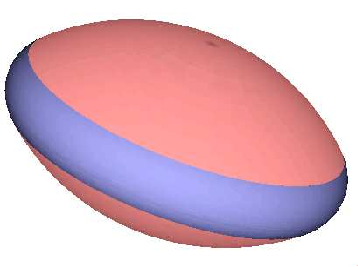
\includegraphics{Figures/snapshot1a}}\quad%
\subfigure[Prolate]
{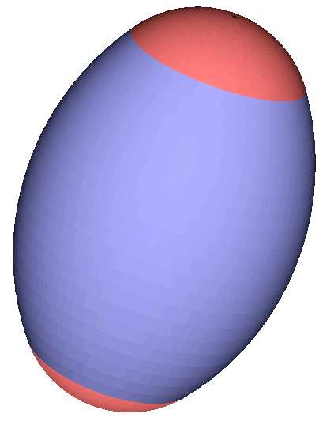
\includegraphics[scale=0.7]{Figures/snapshot1b}}%
\caption{Ovoid particles.}
\label{fig:ovoids}
\end{figure}
%
\item[kshape=6]
nobbies (2D), a non-circular shape that is composed
of clusters of circles
(\hyperref[fig:nobbies]{Fig.~\ref*{fig:nobbies}}).
The particle is neither smooth nor convex.
\begin{figure}
\centering

\includegraphics[scale=1.00]{Figures/Nobby_5_03_085}
\caption{Nobby particle: \texttt{nobs=5}, 
                          \texttt{satrad=0.30}, and \texttt{cenrad=0.85}}
\label{fig:nobbies}
\end{figure}
%
\item[kshape=7]
bumpies (3D), a non-spherical shape that is composed
of clusters of spheres
(\hyperref[fig:bumpies]{Fig.~\ref*{fig:bumpies}}).
The particle is neither smooth nor convex.
\begin{figure}
\centering
\subfigure[\texttt{nbumps=2}, \texttt{satrad=0.7}, 
           \texttt{cenrad=0.9}, \texttt{cirrad=0.75}]
{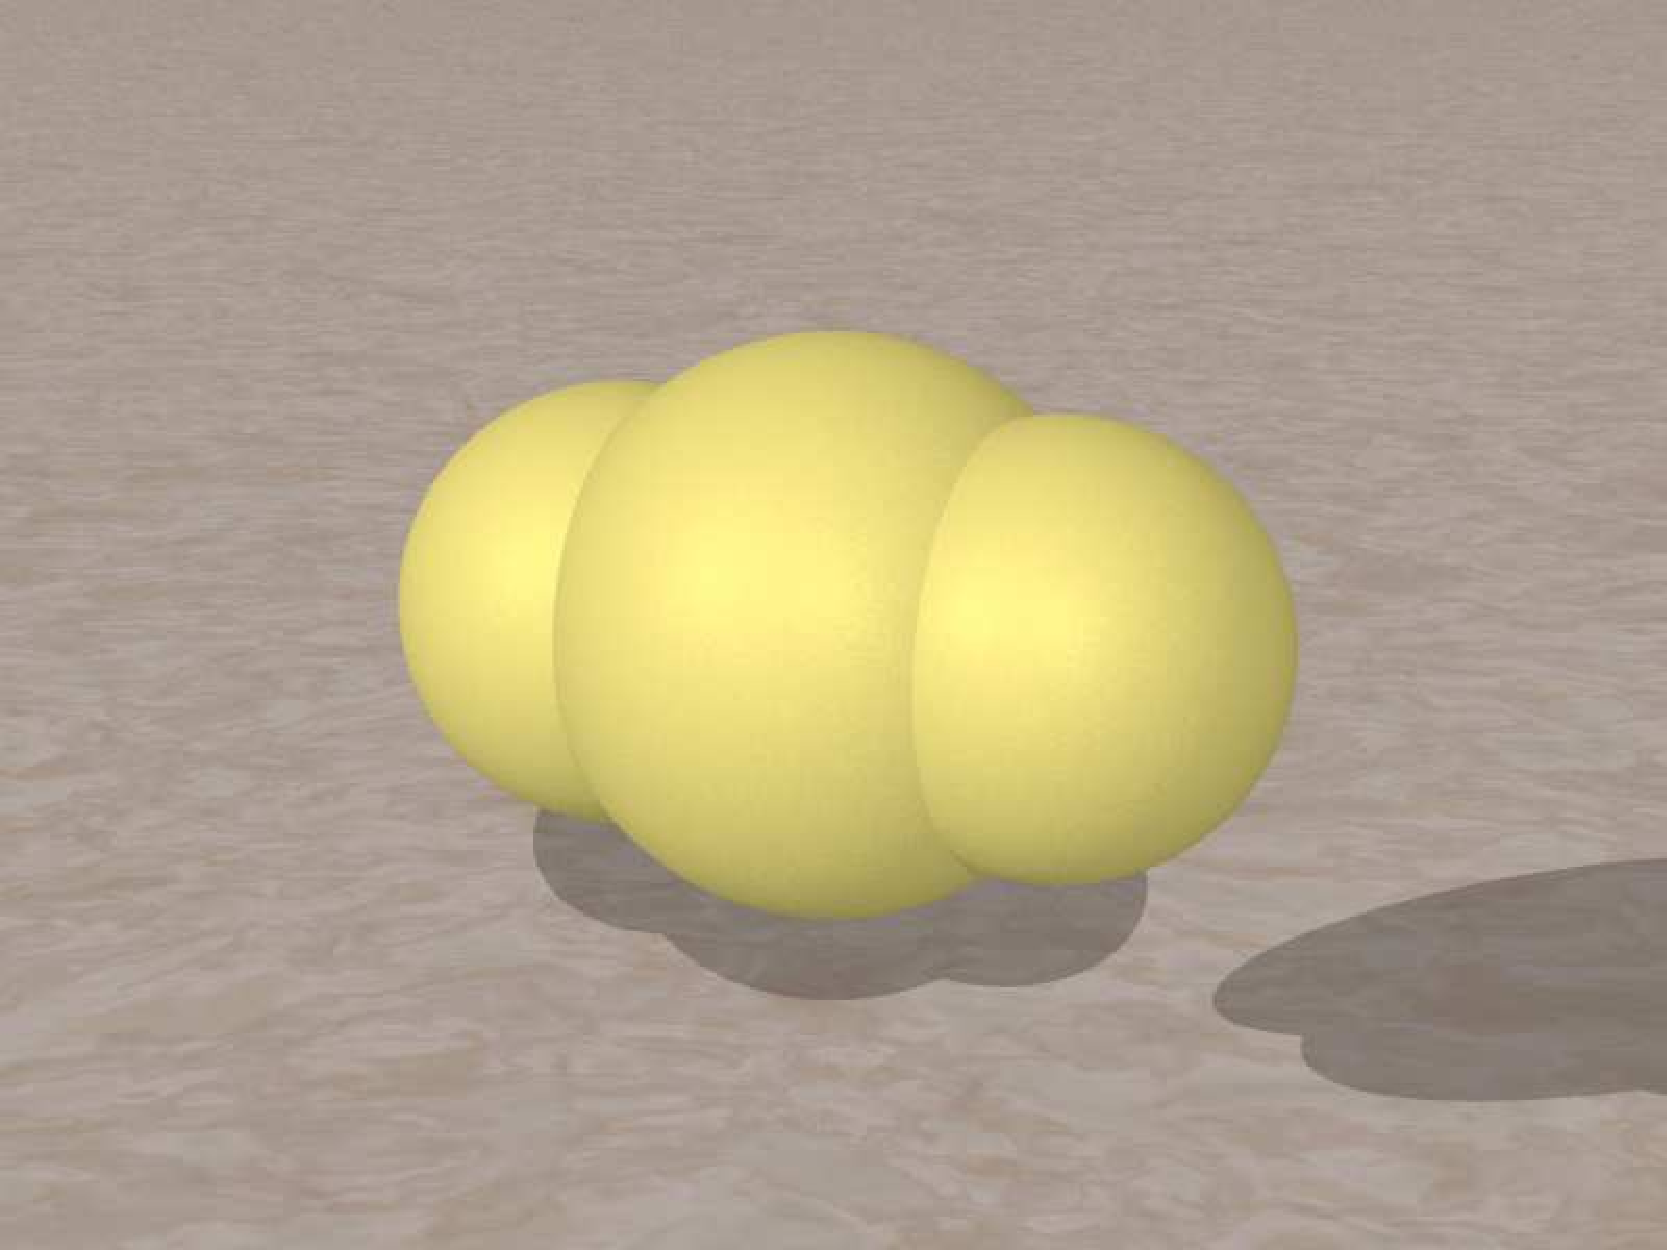
\includegraphics[scale=0.20]{Figures/Bumpy-2-07-09-075-a}}\quad
\subfigure[\texttt{nbumps=3}, \texttt{satrad=0.8}, 
           \texttt{cenrad=1.0}, \texttt{cirrad=0.7}]
{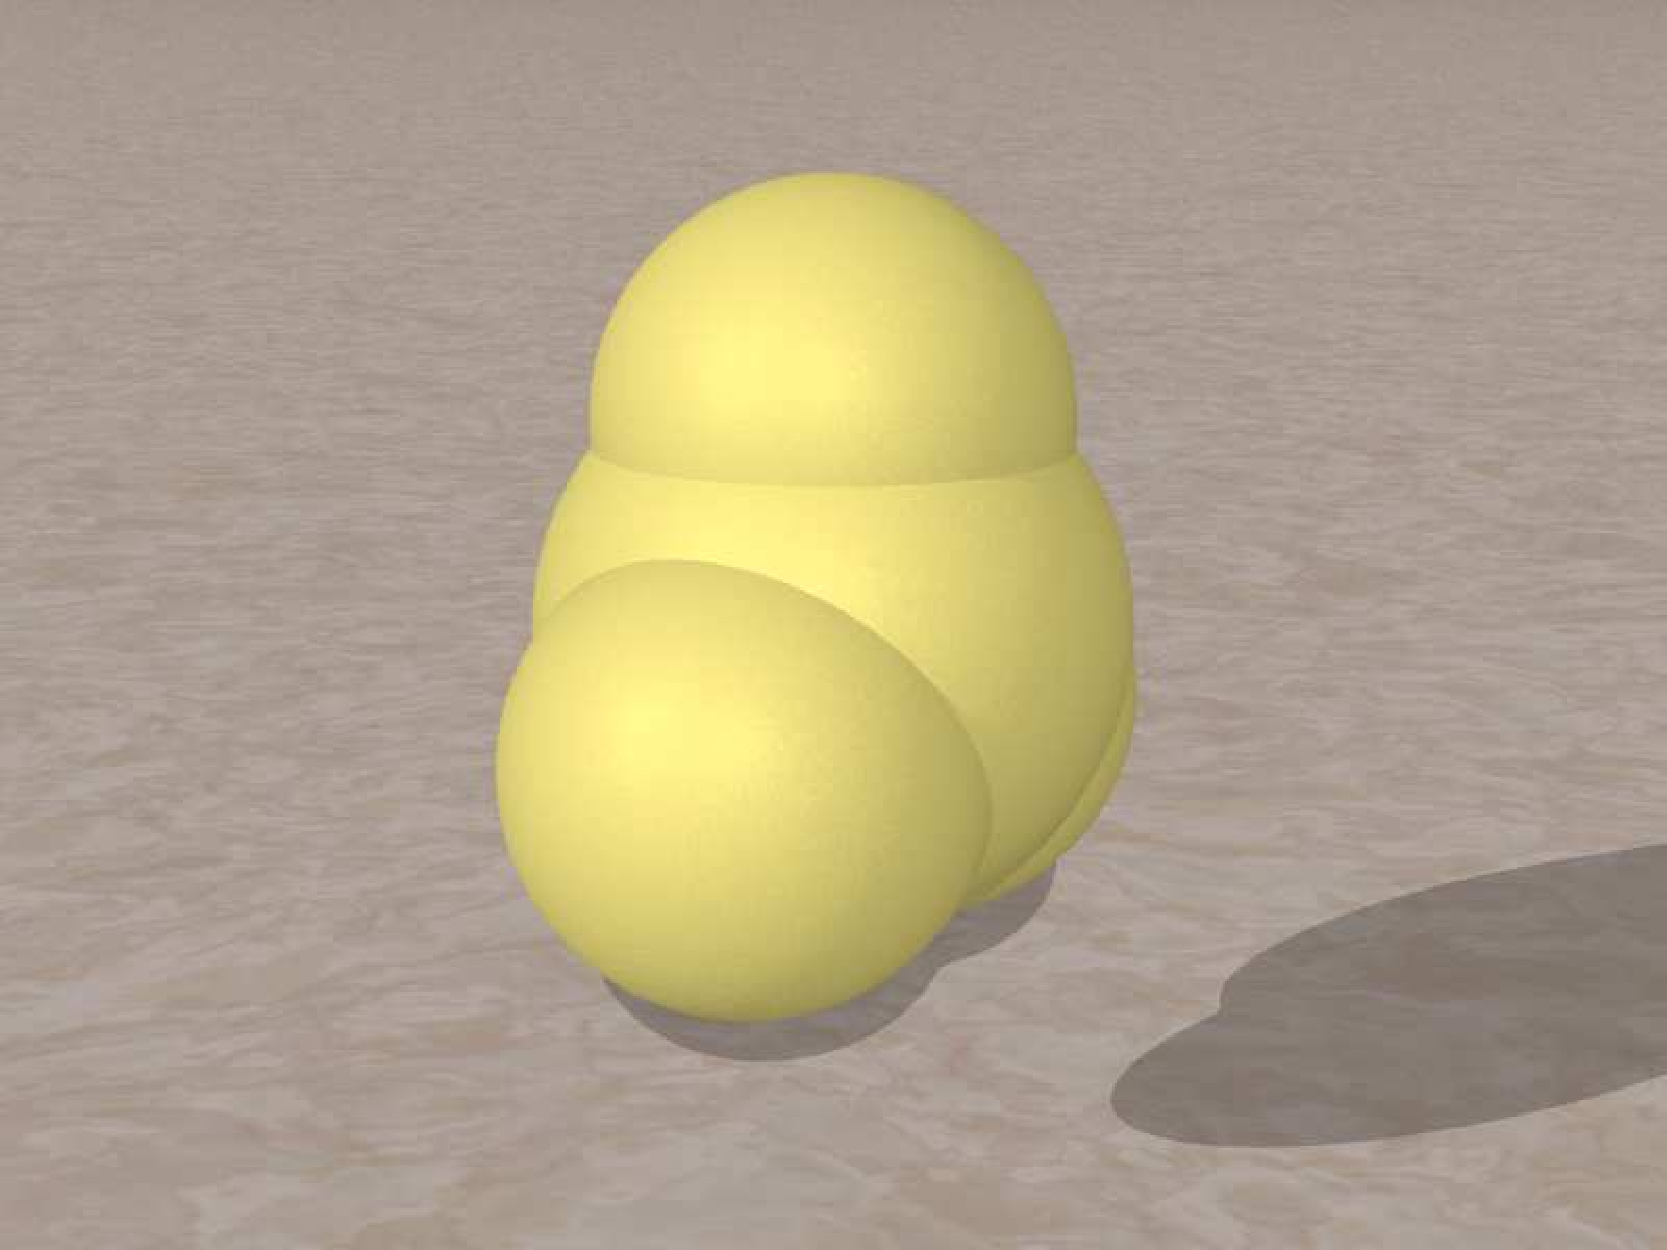
\includegraphics[scale=0.20]{Figures/Bumpy-3-08-10-07-a}}\quad
\subfigure[\texttt{nbumps=4}, \texttt{satrad=0.6},
           \texttt{cenrad=0.8}, \texttt{cirrad=0.7}]
{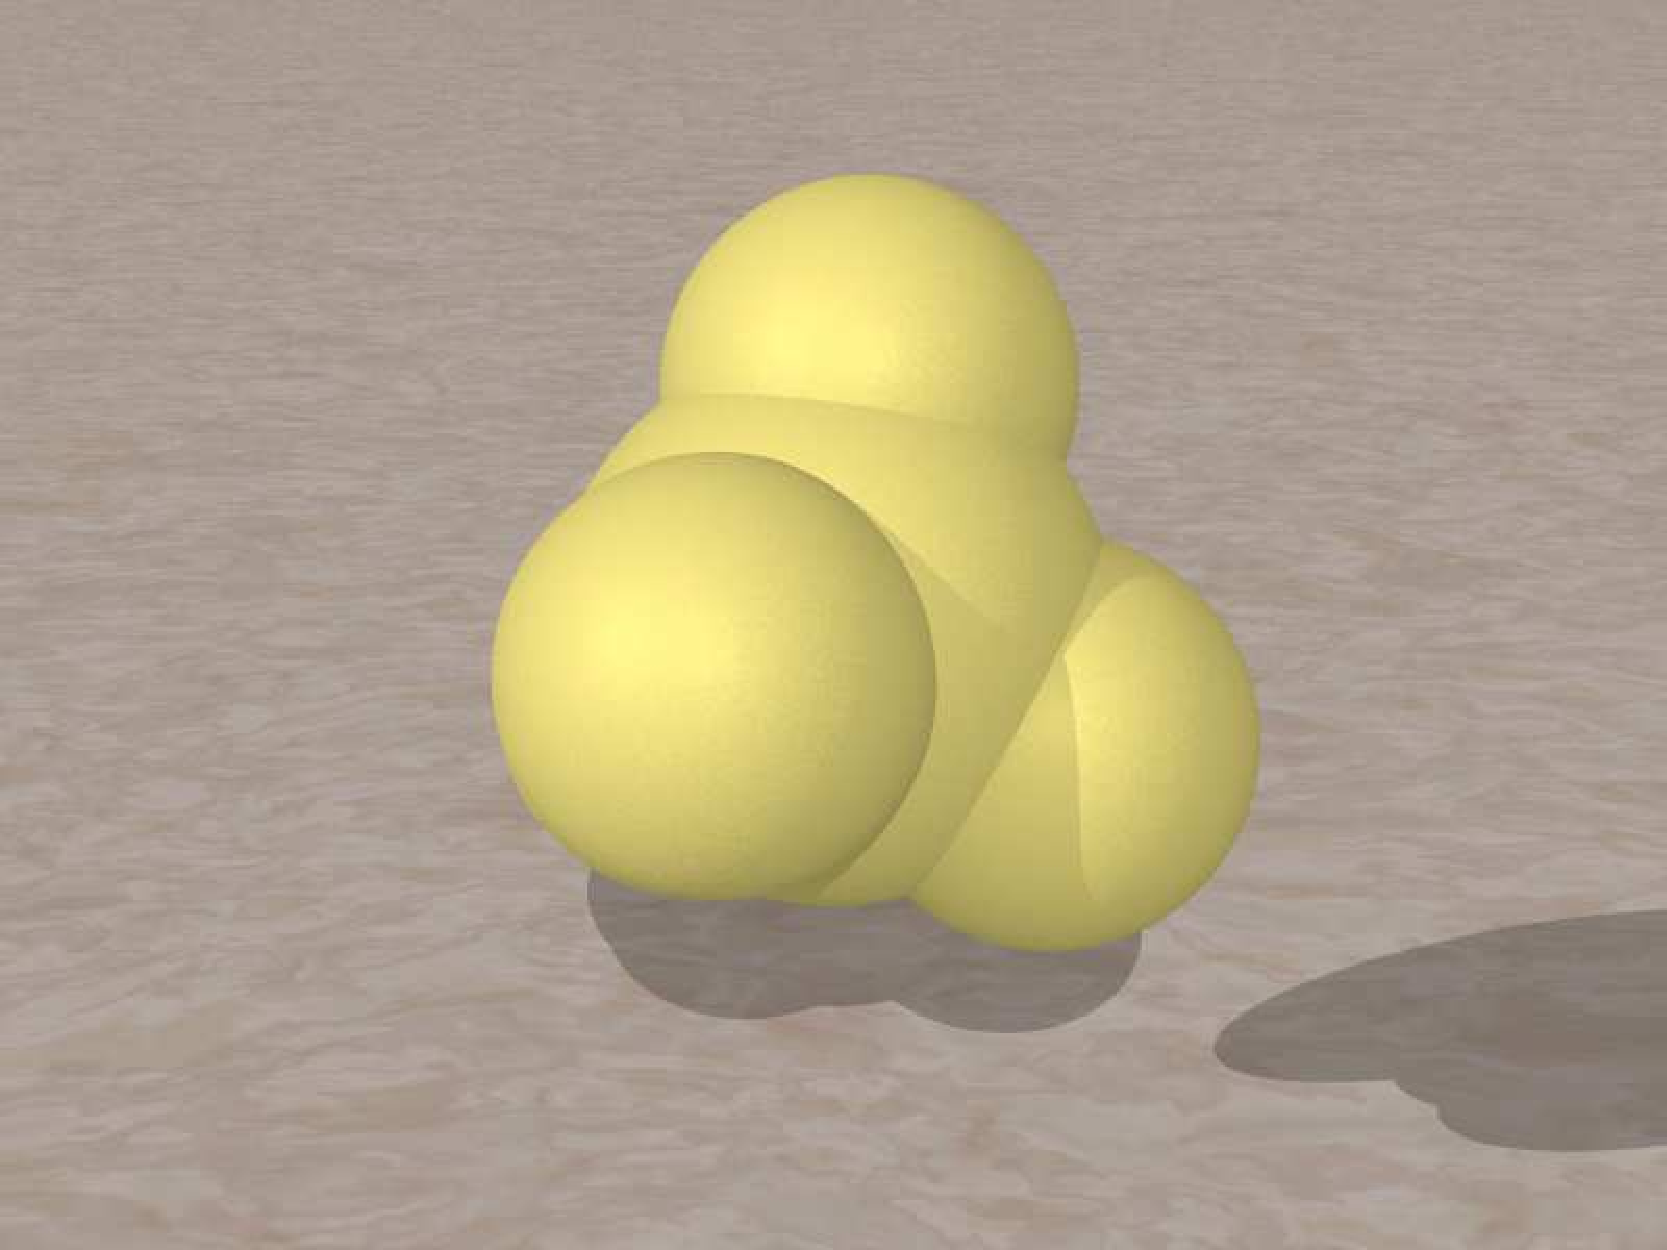
\includegraphics[scale=0.20]{Figures/Bumpy-4-06-08-07-a}}\quad
\subfigure[\texttt{nbumps=6}, \texttt{satrad=0.7},
           \texttt{cenrad=1.0}, \texttt{cirrad=0.6}]
{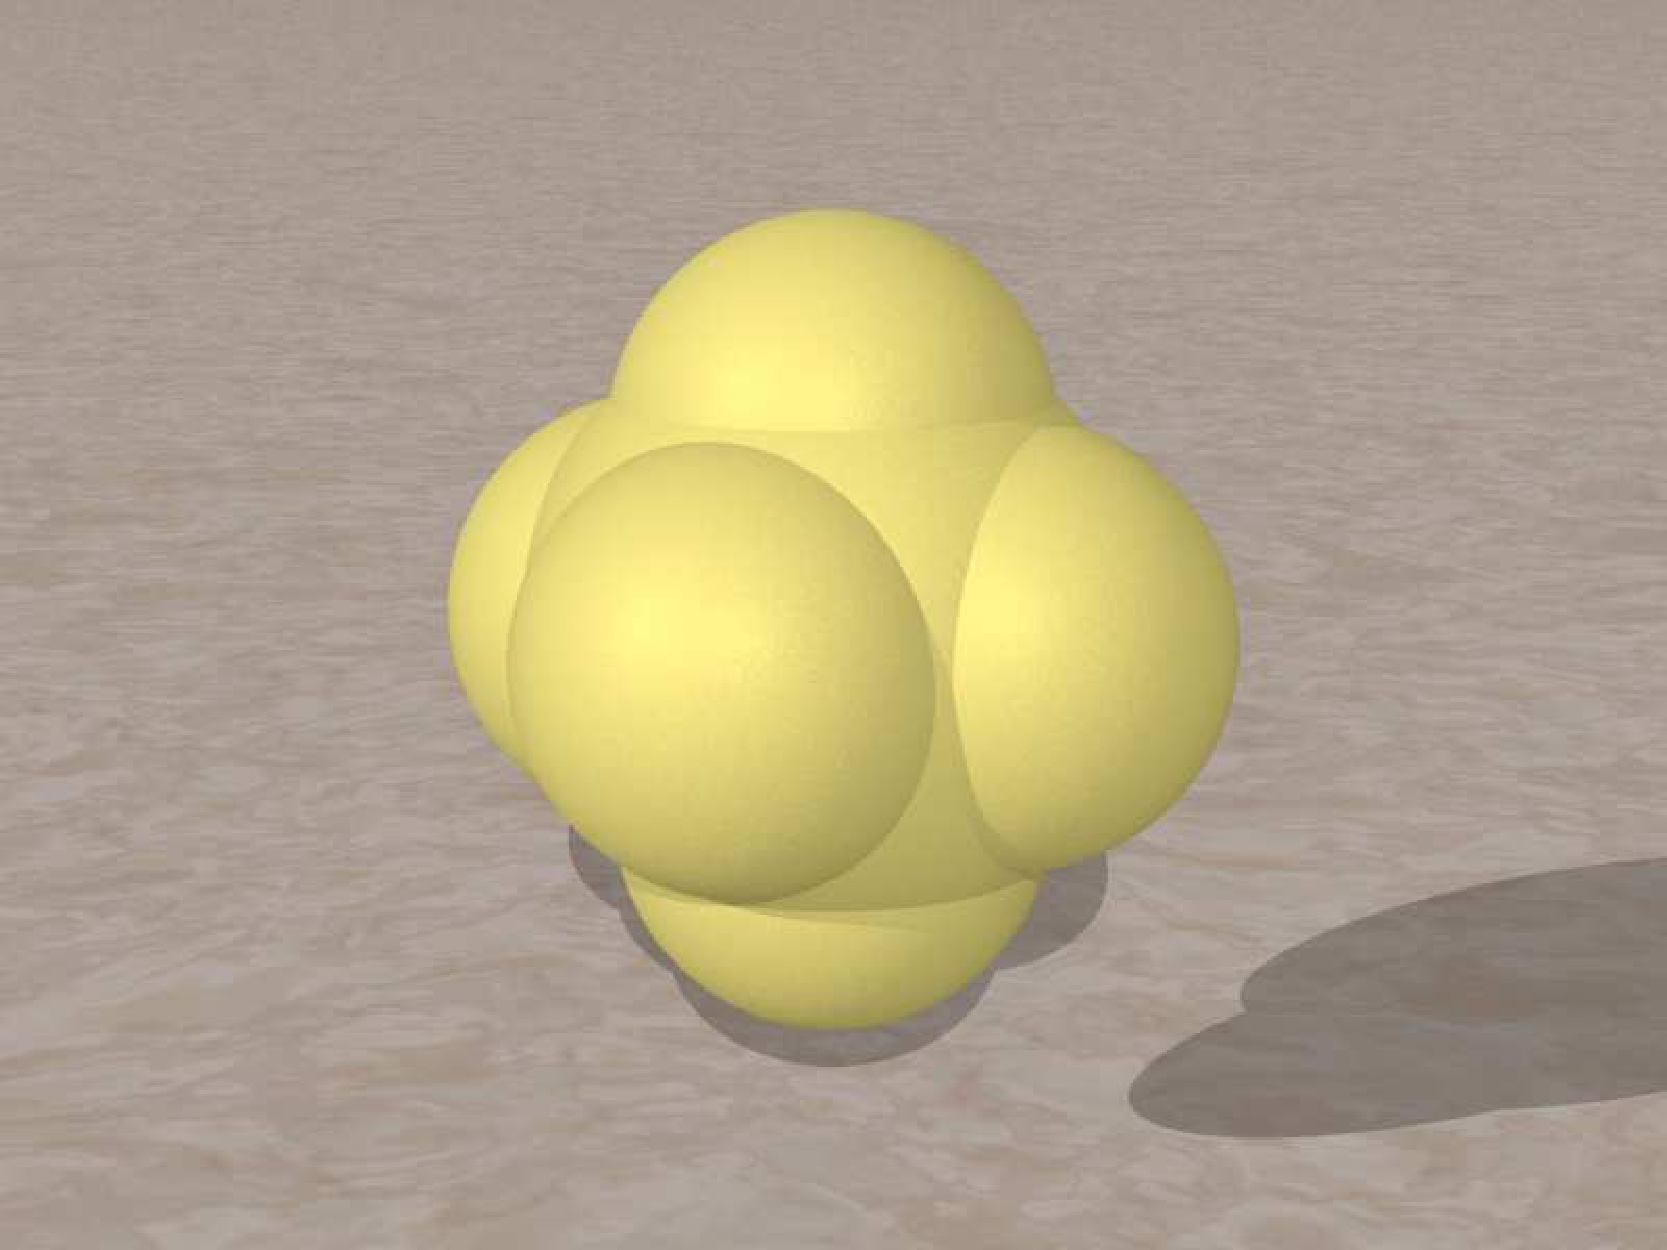
\includegraphics[scale=0.20]{Figures/Bumpy-6-07-10-06-a}}\quad
\subfigure[\texttt{nbumps=8}, \texttt{satrad=0.4},
           \texttt{cenrad=0.9}, \texttt{cirrad=0.8}]
{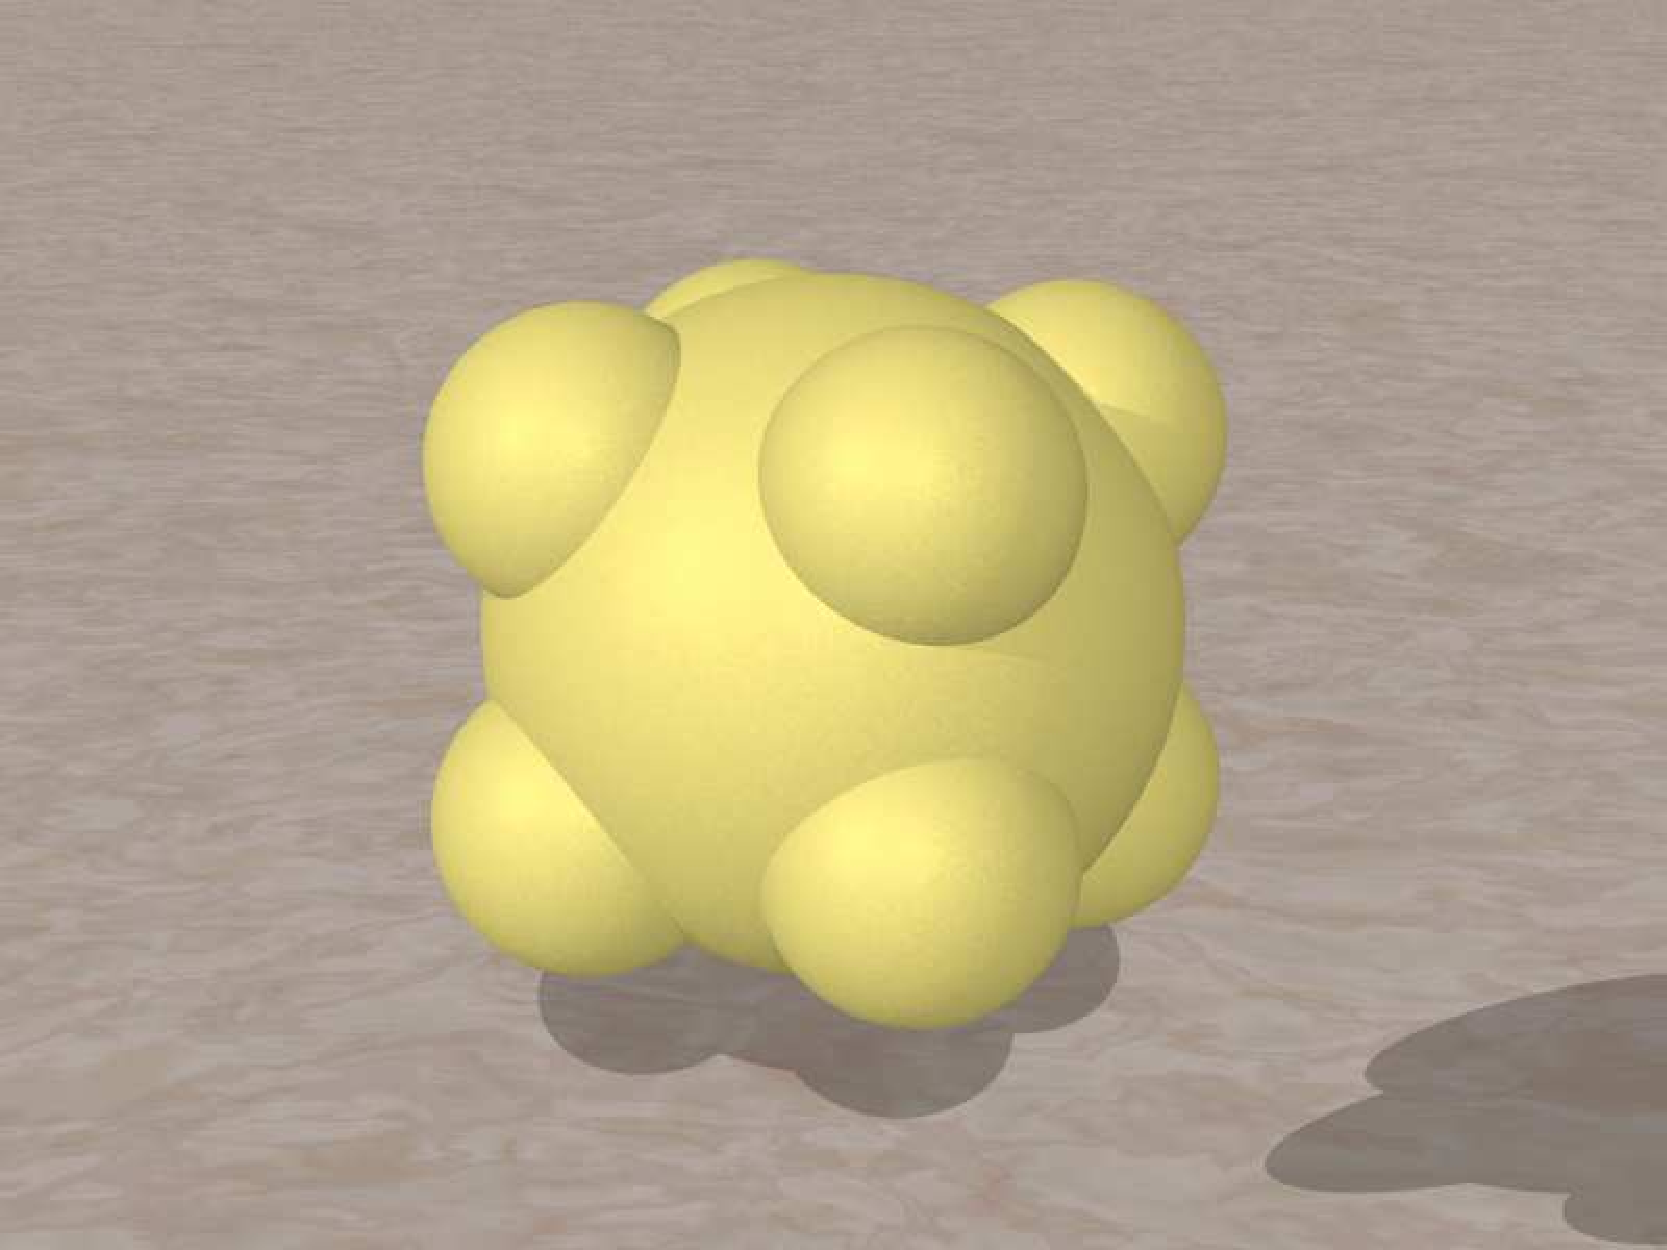
\includegraphics[scale=0.20]{Figures/Bumpy-8-04-09-08-a}}%
\caption{Bumpy particles.}
\label{fig:bumpies}
\end{figure}
\end{Options}
%
\subsubsection[\texttt{np, xcell(1,1)}]{\Var{np,xcell(1,1),xcell(2,2),xcell(3,3)}{i6,3(1pd25.17)}}%
\label{sec:xcell11}
The number of particles, \texttt{np}, 
should appear within the first six columns,
and the three dimensions of the assembly should be presented
in double precision format, with 25 columns per 
dimension (\hyperref[fig:xcells]{Fig.~\ref*{fig:xcells}}).
\begin{figure}
  \centering
  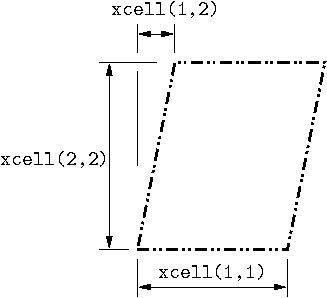
\includegraphics{Figures/xcells.pdf}
  \caption{The \texttt{xcell(i,j)} dimensions for a 2D assembly}
  \label{fig:xcells}
\end{figure}
These dimensions are simply the spacings between opposing periodic
boundaries.
The value of \texttt{xcell(3,3)} must be given, even with
3D assemblies (any value will work, since it will be ignored in the
simulation).
%
\subsubsection[\texttt{xcell(1,2)}]{\Var{xcell(1,2),xcell(1,3),xcell(2,3)}{6x,3(1pd25.17)}}%
\label{sec:xcell12}
After six (blank) columns, the
three shear offsets should be given in double precision format, 
with 25 columns per offset (see the
offset \texttt{xcell(1,2)} in
\hyperref[fig:xcells]{Fig.~\ref*{fig:xcells}}.
%
\subsubsection[\texttt{beta}]{\Var{beta}{1pd25.17}\ --- oval 
and ovoid particles only!}\label{sec:beta}
When 2D ovals or 3D ovoids are being used, this fourth line contains the
splice angle, \texttt{beta}, in \emph{degrees}
(\hyperref[fig:four_arc]{Fig.~\ref*{fig:four_arc}}).
%
\begin{figure}
  \centering
  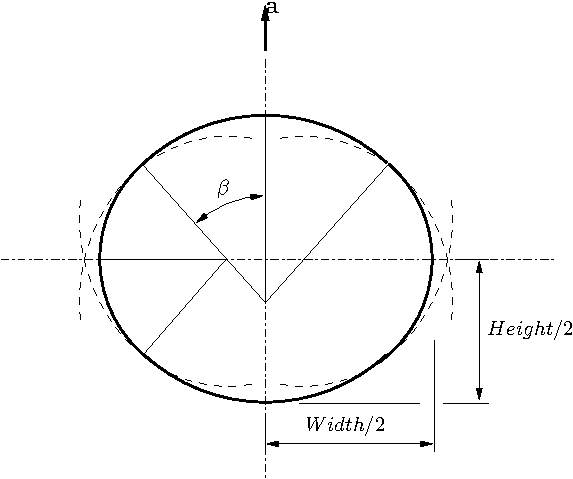
\includegraphics{Figures/four_arc.pdf}
  \caption{Geometry of an oval composed of four circular arcs.}
  \label{fig:four_arc}
\end{figure}
%
The angle $\beta$ must be greater than zero and no greater than $90^{\circ}$.
The particle aspect ratio will be limited by your choice of $\beta$
(Sections~\hyperref[sec:oval_data]{\ref*{sec:oval_data}}.
The height/width ratio must lie within the following bounds:
\begin{equation}
\frac{1-\cos\beta}{\sin\beta} < \alpha <%
\frac{\cos\beta}{1-\sin\beta} \;.
\end{equation}
%
\subsubsection[\texttt{nobs} or \texttt{nbumps}]
              {\Var{nobs \textrm{or} nbumps}{* integer}%
              \ --- nobby (2D) and bumpy (3D)
              particles only!}\label{sec:nobs}
When 2D nobby particles are being used, this line contains the
integer number of satellite circles (arcs) that surround a central circle
(see \hyperref[fig:nobbies]{Section~\ref*{fig:nobbies}}).
The input variable \texttt{nobs} gives the integer number of
satellite circles.  These circles are equally spaced around the
central circles.
The satellite circles are centered on a ``circumscribing circle''
of radius $1.0$.
\par
When 3D bumpy particles are being used, this line contains the
integer number of satellite spheres that surround a central sphere
(see Fig.~\ref{fig:bumpies}).
\Dempla\ currently restricts \texttt{nbumps} to the following five values:
2, 3, 4, 6, or~8, with examples shown in
\hyperref[fig:bumpies]{Fig.~\ref*{fig:bumpies}}.
In each case, the satellite spheres of a bumpy particles will be centered
on the surface of a ``circumscribing sphere'' (i.e., the
satellite spheres are not necessarily centered on the surface of the
central sphere).
The component spheres of bumpy (3D) particles have the following
arrangements:
%
\begin{Options}
\item[nbumps=2]
Two satellite spheres are place on opposite sides of the central sphere,
diametrically opposed.
The satellite spheres are centered on the surface of a ``circumscribing
sphere.''  See \hyperref[fig:bumpies]{Fig.~\ref*{fig:bumpies}}a.
\item[nbumps=3]
Three satellite spheres are placed around the central sphere.
The satellite spheres are centered on the vertices of an equilateral triangle
that is circumscribed by the circumscribing sphere.
That is, the satellite spheres are equally spaced along the equator
of the circumscribing sphere.
See \hyperref[fig:bumpies]{Fig.~\ref*{fig:bumpies}}b.
\item[nbumps=4]
Four satellite spheres are placed around the central sphere.
The satellite spheres are centered on the vertices of a
tetrahedron that is circumscribed by the circumscribing sphere.
That is, the satellite spheres are equally spaced around the full surface
of the circumscribing sphere.
See \hyperref[fig:bumpies]{Fig.~\ref*{fig:bumpies}}c.
\item[nbumps=6]
Six satellite spheres are placed around the central sphere.
The satellite spheres are centered on the vertices of a
octahedron that is circumscribed by the circumscribing sphere.
That is, the satellite spheres are equally spaced around the full surface
of the circumscribing sphere.
See \hyperref[fig:bumpies]{Fig.~\ref*{fig:bumpies}}d.
\item[nbumps=8]
Eight satellite spheres are placed around the central sphere.
The satellite spheres are centered on the vertices of a
cube that is circumscribed by the circumscribing sphere.
That is, the satellite spheres are equally spaced around the full surface
of the circumscribing sphere.
See \hyperref[fig:bumpies]{Fig.~\ref*{fig:bumpies}}e.
%
\end{Options}
%
\par
Regardless of whether nobbies or bumpies are being used, 
this line of input must be followed by a line
that gives relative sizes of the circles or spheres that comprise
a particle, as in the
following section
(\hyperref[sec:satrad]{Section~\ref*{sec:satrad}}).
%
\subsubsection[\texttt{satrad}, \texttt{cenrad}, \texttt{cirrad}]
              {\Var{satrad, cenrad, cirrad}{* double precision}\ --- nobby 
              (2D) bumpy and (3D) particles only!}\label{sec:satrad}
These values are only used with nobby (2D) bumpy (3D) particles, and
they are placed on a single line in double-precision format separated with
spaces.
\par
Every particle in an assembly will have the same shape, but they
can have different sizes.  
Their common shape is specified with the values of \texttt{nobs},
\texttt{nbumps}, \texttt{satrad}, \texttt{cenrad}, and \texttt{cirrad}.
These values give a ``base'' shape and size for the particles.
The actual size of each particle is equal to the common ``base size''
multiplied by an individual scaling radius for each particle
(Sections~\ref{sec:nobby_data} and~\ref{sec:bumpy_data}).
\par
The input variables \texttt{satrad} and \texttt{cenrad} are the
base sizes of the satellite and central circles or spheres of the 
nobby~(2D) and bumpy~(3D) cluster particles.
The input variable \texttt{cirrad} is the radius of circumscribing
sphere, as described in
\hyperref[sec:nobs]{Section~\ref*{sec:nobs}}.
\Dempla\ currently does not support \texttt{cirrad} for 2D nobby particles:
the satellite circles are centered on a circumscribing circle
of radius $1.0$.
%
\subsection{Particle data in \texttt{D}-\textsf{StartFiles}}%
\label{sec:StartFile2}
Following the general information at the head of a 
\texttt{D}\textsf{StartFile}, information is given on each particle,
with one line per particle.  
The arrangement of this data depends upon the type
of particle.
\subsubsection{Circle (disk) particle data}\label{sec:circle_data}
Three fields give the radius,
the $x_{1}$--location, and the $x_{2}$--location of the particle.
The location coordinates refer to the center of the particle.
Following the general information at the head of a
\texttt{D}\textsf{StartFile}, this
information is given for each circle,
with each circle beginning on a new line.
The data items are listed below.
Each data field is in \texttt{1pd25.17} format, with
spaces or a new line between the fields.
The data fields are given as double-precision values
separated by spaces, one particle per line.
The example input on \hyperref[page:dfile]{page~\pageref*{page:dfile}}
shows two lines of data for circular particles.
\begin{itemize}
\item
Radius of the circle.
\item
$x_{1}$--location of the circle's center.
\item
$x_{2}$--location of the circle's center.
\end{itemize}
\subsubsection{Oval particle data}\label{sec:oval_data}
Five fields give the oval width, the ratio of height divided
by the width,
the $x_{1}$--location, the $x_{2}$--location, and the orientation
angle (in \emph{degrees}) of particle, measured counterclockwise
from the $x_{1}$-direction
(\hyperref[fig:orientation_angle]{Fig.~\ref*{fig:orientation_angle}}).
%
\begin{figure}
  \centering
  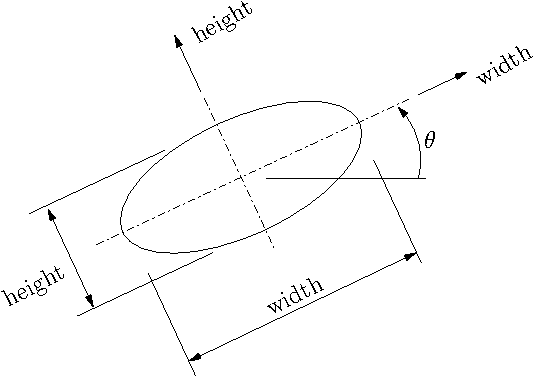
\includegraphics{Figures/orientation.pdf}
  \caption{Orientation angle $\theta$ for elongated particles (2D ovals
           and ellipses).}
  \label{fig:orientation_angle}
\end{figure}
%
The location coordinates refer to the center of the particle.
Following the general information at the head of a
\texttt{D}\textsf{StartFile}, this
information is given for each oval,
with each oval beginning on a new line.
The data items are listed below.
Each data item is given in \texttt{1pd25.17} format, with
spaces or a new line between the fields.
The data fields are given as double-precision values
separated by spaces, one particle per line.
%
\begin{itemize}
\item
Half-width of the oval.  
Note that the oval width may be greater or less than the height
(with ellipses, the width must be greater than its height).  
The width is measured as shown in 
\hyperref[fig:orientation_angle]{Fig.~\ref*{fig:orientation_angle}},
at an angle of $\theta$ counterclockwise
from the horizontal $x_{1}$ axis.
As input, you should give one half of the full particle width.
\item
Ratio of the height divided by the width of the particle
(\hyperref[fig:orientation_angle]{Fig.~\ref*{fig:orientation_angle}}).  
For ovals, the ratio may be greater or less than one.
\item
$x_{1}$--location of the oval's center.
\item
$x_{2}$--location of the oval's center.
\item
Orientation angle $\theta$
of the oval's width (in degrees, 
\hyperref[fig:orientation_angle]{Fig.~\ref*{fig:orientation_angle}}).
\end{itemize}
%
\subsubsection{Ellipse particle data}\label{sec:ellipse_data}
The code for this has not been recently tested
and might not be stable.
Five fields give the major radius, the ratio of the minor radius
divided by the major radius (a number greater than zero, but
no greater than one),
the $x_{1}$-location, the $x_{2}$-location, and the orientation
angle (in \emph{degrees}) of the major axis, measured counterclockwise
from the $x_{1}$-direction
(\hyperref[fig:orientation_angle]{Fig.~\ref*{fig:orientation_angle}}).
The location coordinates refer to the center of the ellipse.
Following the general information at the head of a
\texttt{D}\textsf{StartFile}, this
information is given for each ellipse,
with each ellipse beginning on a new line.
The data items are listed below.
Each data item is given in \texttt{1pd25.17} format, with
spaces or a new line between the fields.
The data fields are given as double-precision values
separated by spaces, one particle per line.
At present, the ellipse width must be greater than its height, with
a height-to-width ratio less than one.
%
\begin{itemize}
\item
Major radius of the ellipse.
\item
Ratio of the minor radius divided by the major radius of the particle
(\hyperref[fig:orientation_angle]{Fig.~\ref*{fig:orientation_angle}}).
For ellipses, the ratio must be greater than zero, but no greater than one.
\item
$x_{1}$--location of the ellipse's center.
\item
$x_{2}$--location of the ellipse's center.
\item
Orientation angle $\theta$ of the ellipse's width (in degrees, \hyperref[fig:orientation_angle]{Fig.~\ref*{fig:orientation_angle}}).
\end{itemize}
%
\subsubsection{Sphere particle data}\label{sec:sphere_data}
Four fields give the radius,
the $x_{1}$--location, the $x_{2}$--location, and the $x_{3}$--location 
of the particle.
The location coordinates refer to the center of the particle.
Following the general information at the head of a
\texttt{D}\textsf{StartFile}, this
information is given for each sphere,
with each sphere beginning on a new line.
The data items are listed below.
Each data item is given in \texttt{1pd25.17} format, with
spaces or a new line between the fields.
The data fields are given as double-precision values
separated by spaces, one particle per line.
%
\begin{itemize}
\item
Radius of the sphere.
\item
$x_{1}$--location of the sphere's center.
\item
$x_{2}$--location of the sphere's center.
\item
$x_{3}$--location of the sphere's center.
\end{itemize}
%
\subsubsection{Ovoid particle data}\label{sec:ovoid_data}
Seven fields give the
ovoid's revolved radius, the ratio of the axial radius divided
by the revolved radius, the location coordinates, and the orientation
angles $\gamma_{1}$ and $\gamma_{2}$ of the ovoid's axis of revolution,
$\mathbf{a}$.
An ovoid is formed by rotating an oval
(i.e. \hyperref[fig:four_arc]{Fig.~\ref*{fig:four_arc}})
about its central axis $\mathbf{a}$.
The location coordinates refer to the center of the particle.
Following the general information at the head of a
\texttt{D}\textsf{StartFile}, this
information is given for each ovoid,
with each ovoid beginning on a new line.
The data items are listed below.
Each data item is given in \texttt{1pd25.17} format, with
spaces or a new line between the fields.
The data fields are given as double-precision values
separated by spaces, one particle per line.
\begin{itemize}
\item
Half of the transverse (revolved, half) width of the ovoid.  
This half-width is measured perpendicular
to the central axis of revolution, $\mathbf{a}$.
\item
Ratio of the axial height divided
by the transverse width.  
The ratio can be greater or less than one, but it must be greater than zero.
Ratios less than one are oblate; ratios greater than one are prolate
(\hyperref[fig:ovoids]{Fig.~\ref*{fig:ovoids}}).
Note that large aspect ratios (or small inverse ratios) require much more
computation time.  I would not recommend using a ratio greater than 2 or
less than 0.5.
\item
$x_{1}$--location of the ovoid's center.
\item
$x_{2}$--location of the ovoid's center.
\item
$x_{3}$--location of the ovoid's center.
\item
$\gamma_{1}$ orientation angle (in radians) of the ovoid's axis
of revolution, $\mathbf{a}$
(\hyperref[fig:coordinates]{Fig.~\ref*{fig:coordinates}}).
This angle should be no less than zero and no greater than
90$^{\circ}$.
\begin{figure}
  \centering
  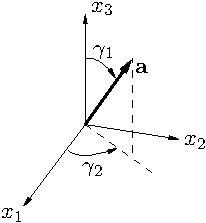
\includegraphics{Figures/coordinates}
  \caption{Orientation angles $\gamma_{1}$ and $\gamma_{2}$ 
           for 3D ovoid particles.
           Vector $\mathbf{a}$ is the central axis of revolution of the ovoid
           (\hyperref[fig:four_arc]{Fig.~\ref*{fig:four_arc}}
           and \hyperref[fig:orientation_angle]{Fig.~\ref*{fig:orientation_angle}}).}
  \label{fig:coordinates}
\end{figure}
\item
$\gamma_{2}$ orientation angle (in radians) of the ovoid's axis
of revolution $\mathbf{a}$
(\hyperref[fig:coordinates]{Fig.~\ref*{fig:coordinates}}).
\end{itemize}
%
%
\subsubsection{Nobby (2D) particle data}\label{sec:nobby_data}
Four fields give the scaling radius, 
the $x_{1}$--location, the $x_{2}$--location, and the orientation
angle (in degrees) of the particle.
The location coordinates refer to the center of the particle.
Following the general information at the head of a
\texttt{D}\textsf{StartFile}, this
information is given for each nobby,
with each nobby beginning on a new line.
The data items are listed below.
Each data item is given in \texttt{1pd25.17} format, with
spaces or a new line between the fields.
The data fields are given as double-precision values
separated by spaces, one particle per line.
%
\begin{itemize}
\item
Scaling radius of the nobby particle.
This scaling radius is multiplied by the base radii,
\texttt{satrad} and \texttt{cenrad}, as described
in \hyperref[sec:satrad]{Section~\ref*{sec:satrad}}.
These products give the actual sizes of the radii that comprise
the nobby particle.
\item
$x_{1}$--location of the nobby particle's center.
\item
$x_{2}$--location of the nobby particle's center.
\item
$\theta_{3}$ orientation angle (in degrees) of the particle.
The center of one of the satellite particles is located at
angle $\theta_{3}$, measured counter-clockwise from the $x_{1}$--direction.
The other satellite circles are equally spaced at angle
\mbox{$360^{\circ}/$\texttt{nobs}}.
\end{itemize}
%
%
\subsubsection{Bumpy (3D) particle data}\label{sec:bumpy_data}
Eight fields give the scaling radius, 
the $x_{1}$--location, the $x_{2}$--location, 
the $x_{3}$--location, and a four-component unit quaternion
of the particle's orientation.
The location coordinates refer to the center of the particle.
Following the general information at the head of a
\texttt{D}\textsf{StartFile}, this
information is given for each bumpy,
with each bumpy beginning on a new line.
The data items are listed below.
Each data item is given in \texttt{1pd25.17} format, with
spaces or a new line between the fields.
The data fields are given as double-precision values
separated by spaces, one particle per line.
%
\begin{itemize}
\item
Scaling radius of the bumpy particle.
This scaling radius is multiplied by the base radii
(\texttt{satrad}, \texttt{cenrad}, and \texttt{cirrad}) as described
in \hyperref[sec:satrad]{Section~\ref*{sec:satrad}}.
These products give the actual sizes of the radii that comprise
the nobby particle.
\item
$x_{1}$--location of the nobby particle's center.
\item
$x_{2}$--location of the nobby particle's center.
\item
$x_{3}$--location of the nobby particle's center.
\item
$\mathtt{Qp}_{1}$ orientation quaternion of the particle.
\item
$\mathtt{Qp}_{2}$ orientation quaternion of the particle.
\item
$\mathtt{Qp}_{3}$ orientation quaternion of the particle.
\item
$\mathtt{Qp}_{4}$ orientation quaternion of the particle.
\end{itemize}
%
%
\section{Text output files from \Dempla}\label{sec:MacroOutput}
While \Dempla\ is running,
output is periodically written to files.
In Mode~1 (analysis of a single assembly),
two output files are produced:
an A-file and a B-file.
In Mode~2 (wave propagation analysis),
several output files with a \texttt{Results\_} prefix
give information about the multiple DEM assemblies (RVEs)
that comprise the soil column.
In addition, the Mode~2 parameter \texttt{iABfile} in
the \GFile\ specifies whether to create an
A-file and a B-file for each DEM assembly
(\hyperref[sec:iABfile]{Section~\ref*{sec:iABfile}}).
%
The frequency (number of time steps between writing of output)
is specified with the input variable
\texttt{ipts}
(\hyperref[sec:ipts]{Section~\ref*{sec:ipts}}).
These two files contain macro-data, such as stress and
deformation.
A-files and B-files are described in 
Sections~\hyperref[sec:Afiles]{\ref*{sec:Afiles}}%
--\hyperref[sec:bfiles3d]{\ref*{sec:bfiles3d}}.
%
You can also produce F-files, which will contain micro-level data.
Because F-files can be quite large, each creation of these files must
be triggered by the input value \texttt{imicro} in the
\RunFile\ %
(\hyperref[sec:imicro]{Section~\ref*{sec:imicro}}).
F-files are described in
Sections~\hyperref[sec:ffiles]{\ref*{sec:ffiles}}%
--\hyperref[sec:ffiles3d]{\ref*{sec:ffiles3d}}.
%
\subsection{A-files: macro-data for spreadsheets}\label{sec:Afiles}
These files contain macro-data, such as stress,
deformation, and fabric from a simulation.
Mode~1 simulation will create a file named 
\texttt{A<}\textsf{RunFile}\texttt{>.txt}, which 
will be referred to as simply an ``A-file''.
The file contains macro-data, such as stress,
deformation, and fabric.
In Mode~2, an A-file can be created for each DEM assembly,
by setting the parameter \texttt{iABfile} equal to a non-zero
integer in the \GFile\ %
(\hyperref[sec:iABfile]{Section~\ref*{sec:iABfile}}).
The frequency (number of time steps between writing of output)
is specified with the \RunFile\ variable
\texttt{ipts} for Mode~1
(\hyperref[sec:ipts]{Section~\ref*{sec:ipts}}),
and by the \GFile\ variable \texttt{nDEM\_out} in
for Mode~2
(\hyperref[sec:nDEMout]{Section~\ref*{sec:nDEMout}}).
%
\par
The fields in an A-file are separated by Tab characters, 
so that A-files can
be imported into a spreadsheet (note: \emph{imported} not opened).
When importing, you will want to specify the columns as being "tab separated."
The spreadsheet is headed with some general information about the simulation,
followed by a history of time, strains, and stresses.
The strains are reported with the simple measure
%
\begin{equation}\label{eq:strain}
F_{ij} - \delta_{ij}
\end{equation}
%
where $F_{ij}$ are components of the deformation gradient tensor.
Note that the shear deformations are reported as shear angles,
like $F_{12}$, or 
twice the shear strain (a $\gamma$-strain, not an $\varepsilon$-strain).
Stresses and strains are reported at the interval
\texttt{ipts},
which may differ for each segment
of the deformation-stress path 
(Sections~\hyperref[sec:runfile2]{\ref*{sec:runfile2}}
and~\hyperref[sec:ipts]{\ref*{sec:ipts}}).
%
\par
For 2D assemblies, the A-file includes information on the assembly's
particle graph \citep{Satake:1992a,Satake:1993b,Kuhn:1999a}.
This information includes the numbers of vertices (particles that are included
in the particle graph), edges (contacts between particles),
and face (void cells).
\par
For both 2D and 3D assemblies, the A-file includes information on
the \emph{fabric tensor} for the assembly \citep{Satake:1982a}.
We will refer to the fabric tensor with the symbol $\mathbf{A}$, which
is defined with a sum over contacts 
within the assembly.  Note that in an A-file, this tensor
$\mathbf{A}$ is unfortunately labeled as ``\texttt{F}'', with the components
\texttt{F(1,1)}, \texttt{F(2,2)}, etc.
\begin{equation}\label{eq:fabric1}
A_{ij} = \frac{1}{N}
\sum_{k=1}^{N}
n_{i}^{k} n_{j}^{k}\;,
\end{equation}
where $\mathbf{n}^{k}$ is the (unit vector) direction of the 
$k$th branch vector (contact),
and $N$ is the number of contacts in the assembly.
When computing~(\ref{eq:fabric1}), $N$ includes only
those contacts between particles that each have at least 2 contacts
(2D assemblies) or 3 contacts (3D assemblies).
\par
For both 2D and 3D assemblies, the A-file also includes information
on the fabric tensor $\mathbf{A}^{s}$ of only those (``strong'') contacts that
carry a greater-than-average force.
Note that in an A-file, this tensor
$\mathbf{A}$ is unfortunately labeled as ``\texttt{Fs}'', with the components
\texttt{Fs(1,1)}, \texttt{Fs(2,2)}, etc.
This tensor is defined as a sum over the strong contacts within
the assembly:
\begin{equation}\label{eq:fabric2}
A_{ij}^{s} = \frac{1}{N}
\sum_{k\in \mathcal{S}}
n_{i}^{k} n_{j}^{k}\;,
\end{equation}
Where the set of contacts $\mathcal{S}$ is a set of contacts $k$:
\begin{equation}
\mathcal{S} = \{k: |\mathbf{f}^{k}| > \overline{f} \}
\end{equation}
that have a force magnitude $|\mathbf{f}^{k}|$ greater than average:
\begin{equation}
\overline{f} = \sqrt{
\frac{\sum_{k=1}^{N} |\mathbf{f}^{k}|^{2}} {N}
                    }
\end{equation}
The A-file also reports the proportion $v$ of strong contacts in the assembly.
\par
An A-file contains several more columns of data.  The labels of these
columns explain their content, and many are given the same names as
quantities that are described below for B-files
(\hyperref[sec:Bfiles]{Section~\ref*{sec:Bfiles}}).
%
\subsection{B-files: macro-data text files}\label{sec:Bfiles}
These files contain macro-data, such as stress,
deformation, and fabric from a simulation.
A Mode~1 simulation will create a file named 
\texttt{B<}\textsf{RunFile}\texttt{>}, which 
will be referred to as simply an ``B-file''.
The file contains macro-data, such as stress,
deformation, and fabric.
In Mode~2, a B-file can be created for each DEM assembly,
by setting the parameter \texttt{iABfile} equal to a non-zero
integer in the \GFile\ %
(\hyperref[sec:iABfile]{Section~\ref*{sec:iABfile}}).
The frequency (number of time steps between writing of output)
is specified with the \RunFile\ variable
\texttt{ipts} for Mode~1
(\hyperref[sec:ipts]{Section~\ref*{sec:ipts}}),
and by the \GFile\ variable \texttt{nDEM\_out} in
for Mode~2
(\hyperref[sec:nDEMout]{Section~\ref*{sec:nDEMout}}).
\par
The \texttt{B<}\textsf{RunFile}\texttt{>} (or just ``B''-files)
contain more information than A-files---not only 
stresses and deformations, but information
that reflects the numerical performance of the simulation.
For example, the B-file contains information that can characterize
whether the simulation was nearly pseudo-static
(\texttt{chi1}, \texttt{chi2}, \texttt{chi3}, \texttt{chi4}, and
\texttt{knrgy}), 
the relative importance
of viscous damping during the simulation
(\texttt{chi3}, \texttt{chi4}, \texttt{viscbt}, and \texttt{viscct}),
and whether the controlled stresses
were maintained near their target values (\texttt{psi}).
This information, although useful, is packed into a text (ASCII) file
that can be somewhat difficult to read and understand.
B-files are described in the following two sections.
%
\subsection{B-files with 2D simulations}\label{sec:bfile2d}
The first four lines in a B-file contain the following 
four pieces of information in the form of
\texttt{format(i4,2x,a50,2x,a20)}:
\begin{itemize}
\item
an integer that indicates the format (version) of the B-file
 (\texttt{i4} format).
For example, whether the file is for a 2D or 3D simulation,
since B-files 2D and 3D will contain different information.
\item
the name of the \textsf{StartFile} that was used for the simulation
(\hyperref[sec:RunOval]{Section~\ref*{sec:RunOval}}
and \hyperref[sec:startfileD]{Section~\ref*{sec:startfileD}})
%
\item
the version of the \Dempla\ source code
\item
the RVE number (\texttt{i4.4} format).
For Mode~1 simulation, this number is \texttt{0001}.
For Mode~2 simulations, the RVE number begins with \texttt{0001}
for the bottom-most RVE in the soil column to \texttt{nRVEs}
for the top-most RVE (see 
\hyperref[sec:nRVEs]{Section~\ref*{sec:nRVEs}}).
%
\end{itemize}
\par
These for lines are followed by the results of each output cycle,
which occur
at the frequency \texttt{ipts} for Mode~1
(see Section~\ref{sec:ipts}) or \texttt{nDEM\_out}
for Mode~2 
(see \hyperref[sec:nDEMout]{Section~\ref*{sec:nDEMout}}).
\par
For 2D simulations, the information for each output cycle is packed
into just three lines, such as the following:\\[-2ex]
\par\noindent
\footnotesize\normalfont
\begin{verbatim}
1.0320000E-04   5.948067E-05 -1.984000E-04  0.000000E+00  4.212188E-04     1623
  6.49E-04     -1.551593E+04 -2.071540E+04 -2.774535E+01  9.690910E+00 3.29E-07
  1.03E-03 0.00E+00 7.11E-04  6.519467E-03  5.346882E-02  2.655151E+00     3.00
\end{verbatim}
\normalsize\normalfont
\par\noindent
\rule{0ex}{3ex}The contents of these three lines
correspond to the following variables (some of these
are, in fact, arrays):\\[-2ex]
\footnotesize\normalfont
\begin{verbatim}
  timer         defout(1,1)   defout(2,2)   defout(1,2)    knrgy         ntacts
   chi1         stress(1,1)   stress(2,2)   stress(1,2)    pnrgy           psi 
   chi2    chi3     chi4      viscbt        slidet         work1t        xloops
\end{verbatim}
\normalsize\normalfont
\rule{0ex}{3ex}that are given in the following formats:\\[-2ex]
\footnotesize\normalfont
\begin{verbatim}
 1pe14.7,   1x,  1pe14.6,     1pe14.6,      1pe14.6,       1pe14.6,       i9,/,
 2x,1pe9.2, 4x,  1pe14.6,     1pe14.6,      1pe14.6,       1pe14.6,   1pe9.2,/,
 2x,1pe9.2, 1pe9.2, 1pe9.2,   1pe14.6,      1pe14.6,       1pe14.6,   0pf9.2
\end{verbatim}
\normalsize\normalfont
\rule{0ex}{3ex}The various output values are now described.
%
\subsubsection{\texttt{timer}}
The accumulated time, which advances by an amount \texttt{dt} with each
deformation step
(\hyperref[sec:dt]{Section~\ref*{sec:dt}}).
%
\subsubsection{\texttt{defout(i,j)}}\label{sec:defout}
The output values, \texttt{defout(i,j)}, are the difference
between the deformation gradient matrix $F_{ij}$ and the
identity (Kronecker) matrix $\delta_{ij}$, as in
\hyperref[eq:strain]{Eq.~\ref*{eq:strain}} on
\hyperref[eq:strain]{page~\pageref*{eq:strain}}.
For example, the output
\begin{verbatim}
     defout(1,1) =  0.001
     defout(2,2) = -0.002
     defout(1,2) =  0.003
\end{verbatim}
for a 2D assembly corresponds to the following deformation gradient:
\begin{equation}
\mathbf{F} = \left[
\begin{array}{cc}
1.001 & 0.003\\
0     & 0.998
\end{array}
\right]
\end{equation}
The deformation gradient $\mathbf{F}$ is referenced to the initial
assembly (except when the simulation is started with
a C-\StartFile, in which case, $\mathbf{F}$ is carried over
from a previous run).
%
\subsubsection{\texttt{knrgy}}
The kinetic energy of particle motions per unit of the assembly's 
original volume.  
The kinetic energy is computed from both 
translational and rotational velocities of the particles:
\begin{equation}
\frac{1}{\mathrm{Initial\ volume}}
\times
\frac{1}{2}
\sum_{\text{Particles}} \left(
m \bar{\mathbf{v}}^{2} + I \bar{\boldsymbol{\omega}}^{2}
\right)\;,
\end{equation}
where $m$ and $I$ are the mass and the mass moment of inertia of a particle, 
and $\bar{\mathbf{v}}$ and $\bar{\boldsymbol{\omega}}$ are the
average velocity and angular velocity of a particle 
(the averages of the velocities at the two times
$t-dt/2$ and $t+dt/2$).
The energy \texttt{knrgy} is not really meaningful
when \texttt{algori=2}
(see \hyperref[sec:algori]{Section~\ref*{sec:algori}}).
Note that $F_{ij}=0$ for $i>j$, as is the case
in \hyperref[fig:xcells]{Fig.~\ref*{fig:xcells}}.
%
\subsubsection{\texttt{ntacts}}
The number of contacts.  Here, a contact is shared by two particles.  If you
prefer to count a contact twice (once for each of the two particles,
as in 
\hyperref[table:assemblies]{Table~\ref*{table:assemblies}}, then
the number of contacts is, instead, \texttt{ntacts}$\times2$.
%
\subsubsection{\texttt{chi1}}\label{sec:chi1}
One of four measures for determining whether the simulation is nearly
pseudo-static.
The property \texttt{chi1} is the average force imbalance on a particle
divided by the average magnitude of a contact force.
Small values signify that the particles were nearly in equilibrium 
during the deformation process.
When \texttt{algori=2},
the variables \texttt{chi1} and \texttt{chi2}
(\hyperref[sec:chi2]{Section~\ref*{sec:chi2}})
are used as a near-equilibrium criteria
for controlling the pace at which the deformation is allowed to proceed
(\hyperref[sec:algori]{Section~\ref*{sec:algori}}
and \hyperref[sec:xloops]{Section~\ref*{sec:xloops}}).
If there are no contacts within the assembly, then \texttt{chi1} will be zero.
%
\subsubsection{\texttt{stress(i,j)}}
Components of the Cauchy stress tensor.
%
\subsubsection{\texttt{pnrgy}}
The elastic energy stored in the contact springs per unit of the assembly's
original volume.
For the simple linear contact mechanism,
this energy is calculated as
\begin{equation}
\frac{1}{\mathrm{Initial\ volume}}
\times
\frac{1}{2}
\sum_{\text{Contacts}} \left[
\frac{f_{n}^{2}}{k_{n}}
+
\frac{f_{t}^{2}}{k_{t}}
\right]\;,
\end{equation}
where $f_{n}$ and $f_{t}$ are the normal and tangential contact forces,
and $k_{n}$ and $k_{t}$ are the normal and tangential contact
stiffnesses at time $t$.
%
\subsubsection{\texttt{psi}}\label{sec:psi}
This performance measure
characterizes the fluctuation of the controlled stresses from
their intended (target) values. 
When one or more digits in \texttt{icontr} are \texttt{1}'s, then
a servo-control algorithm will attempt
to control certain components of the Cauchy stress 
and maintain them at target values
(see \hyperref[sec:icontr]{Section~\ref*{sec:icontr}}).
The property \texttt{psi} is the sum of the deviations of the controlled
stress components from their
target values divided by the mean stress
(either $1/2$ or $1/3$ $\sigma_{kk}$).
If you are not controlling any of the stress components, then \texttt{psi}
will be zero.
%
\subsubsection{\texttt{chi2}}\label{sec:chi2}
This is another measure of whether the simulation is nearly
pseudo-static
(see \texttt{chi1}, \hyperref[sec:chi1]{Section~\ref*{sec:chi1}}).
The value \texttt{chi2} is the average \emph{moment} imbalance on a 
particle divided by both the average magnitude of a contact force and the
average particle radius.
Small values signify that particles remained nearly in equilibrium 
during a simulation.
%
\subsubsection{\texttt{chi3}}
A measure of whether viscous contact damping could 
have a significant effect
on the reported stresses and deformations.
Its value is the viscous force at an average contact divided
by the average contact force.
%
\subsubsection{\texttt{chi4}}\label{sec:chi4}
A measure of whether viscous body damping could 
be having a significant effect
on the reported stresses and deformations.
Its value is the viscous force on an average particle divided
by the average contact force.
%
\subsubsection{\texttt{viscbt}}
The energy expended in viscous body damping per unit of the
assembly's original volume
(cumulative since the beginning of the simulation).  This quantity may not
be meaningful when \texttt{algori=2}
(see \hyperref[sec:algori]{Section~\ref*{sec:algori}}).
The \emph{increment} in \texttt{viscbt} for a time step $dt$
is computed as follows:
\begin{equation}
\frac{1}{\mathrm{Initial\ volume}}
\times
\sum_{\text{Particles}} \left[
\eta^{v}\mathbf{\bar{v}}\cdot\mathbf{\bar{v}}dt
+
\eta^{\omega}\bar{\boldsymbol{\omega}}\cdot\bar{\boldsymbol{\omega}}dt
\right]\;.
\end{equation}
That is, the increment of work expended in body damping is equal
the damping force ($\eta^{v}\mathbf{v}$) 
multiplied with the particle movement ($\mathbf{v}dt$).
In this equation, $\eta$ is the damping coefficient.
The equation includes separate contributions of translational and
rotational damping.
The velocities $\bar{v}$ and $\bar{\boldsymbol{\omega}}$ are the
averages for a particle at times $t-dt/2$ and $t+dt/2$.
%
\subsubsection{\texttt{slidet}}
The energy expended in frictional sliding per unit of the
assembly's original volume
(cumulative since the beginning of the simulation).
The \emph{increment} in \texttt{slidet} for a time step $dt$
is computed as follows:
\begin{equation}
\frac{1}{\mathrm{Initial\ volume}}
\times
\sum_{\substack{\text{Sliding}\\ \text{contacts}}} \left[
\mu f^{n} \: |\bar{\mathbf{v}}^{\text{contact, }t}|\,dt
\right]\;,
\end{equation}
where $\mu$ is the friction coefficient \texttt{frict},
$f^{n}$ is the normal contact force, and
$\bar{\mathbf{v}}^{\text{contact, }t}$ is the tangential contact
deformation.
The velocity $\bar{\mathbf{v}}^{\text{contact, }t}$
is an average of the velocities at times $t-dt/2$ and $t+dt/2$.
%
\subsubsection{\texttt{work1t}}
The work done by the ``boundary stresses'' per unit of the assembly's
original volume. 
It is computed from the work rate
\begin{equation}
\frac{\mathrm{Current\ volume}}{\mathrm{Initial\ volume}}
\int \sigma_{ij} \dot{F}_{ik} F_{kj}\,dt
\end{equation}
and is cumulative from the beginning of the simulation.
In this equation, $\sigma_{ij}$ is the Cauchy stress.
%
\subsubsection{\texttt{xloops}}\label{sec:xloops}
When \texttt{algori=2}, several time steps will occur 
within each deformation step
(\hyperref[sec:algori]{Section~\ref*{sec:algori}}).
The program self-monitors the number of cycles 
that are required to achieve a near-equilibrium
condition before advancing the assembly deformations.
The property \texttt{xloops} is the average number of cycles that
were required.
\par
The program currently limits the number of cycles
per deformation step to between \texttt{nloop1} and 101
(\hyperref[sec:nloop1]{Section~\ref*{sec:nloop1}}).
When \texttt{xloops} is consistently reported as 3,
the near-equilibrium criteria was met in three or fewer loops
(see \hyperref[sec:algori]{Section~\ref*{sec:algori}}).
When \texttt{xloops} is 101, then the near-equilibrium criteria
were likely not met even after the final cycle.
The threshold, near-equilibrium criteria is currently defined as a value
of $0.5(\mathtt{chi1} + \mathtt{chi2})$ be less than 1\%.
%
\subsubsection{\texttt{viscct}}
This quantity appears in the A-files, but not in the B-files.
The quantity \texttt{viscct} is
the energy expended in viscous contact damping per unit of the assembly's 
original volume
(cumulative since the beginning of the simulation).  This quantity may not be
meaningful
when \texttt{algori=2} (Section~\ref{sec:algori}).
The \emph{increment} in \texttt{viscct} for a time step $dt$
is computed as follows:
\begin{equation}
\frac{1}{\mathrm{Initial\ volume}}
\times
\sum_{\text{Contacts}} \!\!\!\!\left[
\eta^{n}\mathbf{\bar{v}}^{\text{contact, }n}
\cdot\mathbf{\bar{v}}^{\text{contact, }n}
+
\eta^{t}\mathbf{\bar{v}}^{\text{contact, }t}
\cdot\mathbf{\bar{v}}^{\text{contact, }t}
\right]\,dt\;,
\end{equation}
where $\eta^{n}$ and $\eta^{t}$ are the coefficients of contact normal and
contact tangential damping, and
$\mathbf{\bar{v}}^{\text{contact, }n}$ and
$\mathbf{\bar{v}}^{\text{contact, }t}$ are the components of
contact deformation velocities in the normal and tangential directions.
That is, the contribution to \texttt{viscct} of a single contact
is the contact damping force
$\eta\mathbf{\bar{v}}^{\text{contact}}$
multiplied by the displacement increment
$\mathbf{\bar{v}}^{\text{contact}}dt$.
%
\subsection{B-files with 3D simulations}\label{sec:bfiles3d}
As with 2D simulations,
the first four lines of a B-file
contains a file-type identifier, the name of the \textsf{StartFile},
the version of the \Dempla\ source code,
and the RVE number
(see \hyperref[sec:bfile2d]{Section~\ref*{sec:bfile2d}}).
These four lines are followed with results for each output cycle.
With 3D simulations, the information for each output cycle is packed
into five lines.
However, with simulations with a poromechanic model
(\texttt{iporo =} 1, 3, or 4),
six lines are given.
We first describe the five lines, such as the following:\\[-2ex]
\par
\footnotesize
\begin{verbatim}
2.6000000E-05   5.313745E-06 -5.000000E-05  0.000000E+00  6.161242E-05   5168
      9.65E-05  0.000000E+00  0.000000E+00  0.000000E+00  4.39854321784E+02
      1.13E-04 -5.684897E+05 -6.075969E+05 -5.778599E+05  2.12654326770E-02
      0.00E+00 -2.138418E+04  5.103270E+03 -1.097130E+04  2.57476543228E+01
      6.82E-05      5.10E-07  2.169865E-02  0.000000E+00         30.00
\end{verbatim}
\normalsize
\par
\rule{0ex}{3ex}These contents correspond to the following variables (some of these
are, in fact, arrays):\\[-2ex]
\footnotesize
\begin{verbatim}
  timer         defout(1,1)   defout(2,2)   defout(3,3)    knrgy       ntacts
      chi1      defout(1,2)   defout(1,3)   defout(2,3)    pnrgy
      chi2      stress(1,1)   stress(2,2)   stress(3,3)    slidet
      chi3      stress(1,2)   stress(1,3)   stress(2,3)    work1t
      chi4           psi         viscbt       viscct       xloops
\end{verbatim}
\normalsize
\rule{0ex}{3ex}given in the following formats:\\[-2ex]
\footnotesize
\begin{verbatim}
 1pe14.7,  1x,  1pe14.6,      1pe14.6,      1pe14.6,       1pe14.6,       i7,/,
 1pe15.2,       1pe14.6,      1pe14.6,      1pe14.6,       1pe19.11,         /,
 1pe15.2,       1pe14.6,      1pe14.6,      1pe14.6,       1pe19.11,         /,
 1pe15.2,       1pe14.6,      1pe14.6,      1pe14.6,       1pe19.11,         /,
 1pe15.2,       1pe14.2,      1pe14.6,      1pe14.6,       0pf14.2
\end{verbatim}
\normalsize
\par\noindent
\rule{0ex}{3ex}These output fields were described in the previous section
(\ref{sec:bfile2d}).
\par
When a poromechanic model is used (\texttt{iporo = } 1, 3, or 4),
then a sixth line is added with five items, for example:\\[-2ex]
\begin{verbatim}
       1.430419E+04  4.056670E-03  1.9403765E-02  1.8747376E-03 9.935762272E-01
\end{verbatim}
\par\noindent
\rule{0ex}{3ex}with the following information:\\[-2ex]
\begin{verbatim}
       pfluid        defw          fpnrgy         spnrgy        S_now
\end{verbatim}
\par\noindent
\rule{0ex}{3ex}with the following format:\\[-2ex]
\begin{verbatim}
   5x,1pe14.6,       1pe14.6,      1pe15.7,       1pe15.7,      1pe16.9
\end{verbatim}
\par\noindent
\rule{0ex}{3ex}and these five poromechanic items are described below.
%
\begin{itemize}
\item
\texttt{pfluid} is the pore fluid pressure relative to atmospheric pressure;
\item
\texttt{defw} is the inflow of fluid into the assembly
per unit of original pore volume.
\item
\texttt{fpnrgy} is the potential energy of the fluid.
\item
\texttt{spnrgy} is the potential energy imparted to the
grains by the fluid pressure.
\item
\texttt{S\_now} is the fluid water saturation.
\end{itemize}
%
\subsection{F-files: micro-data text files}\label{sec:ffiles}
F-files contain information on the positions of all particles
and the status of all contact forces.
In Mode~1,
these files are created during an \Dempla\ simulation
by setting \texttt{imicro=1} within a deformation-stress segment
of the \RunFile\ %
(\hyperref[sec:imicro]{Section~\ref*{sec:imicro}}).
With \texttt{imicro=1}, a set of F-files will be created at the \emph{start}
of the particular deformation-stress segment.
As many as four separate F-files will be produced, with each containing
a different type of information
(\hyperref[table:ffiles]{Table~\ref*{table:ffiles}}).
The files can be quite large:  for an assembly of 1000 particles, 
a set of 2D F-files is about 300kBytes.
The \FFile\ s can be created when \Dempla\ is run in Mode~2.
\begin{table}
\centering
\begin{tabular}{l|ll}
\hline
\hline
\multicolumn{1}{c}{} & File name & Content\\
\hline
   & \texttt{Fa?<}\RunFile\texttt{>} & Assembly size \\
2D & \texttt{Fb?<}\RunFile\texttt{>} & Particle data \\
   & \texttt{Fc?<}\RunFile\texttt{>} & Contact data \\
   & \texttt{Fd?<}\RunFile\texttt{>} & Void cell data \\
\hline
   & \texttt{Fa?<}\RunFile\texttt{>} & Assembly size \\
3D & \texttt{Fb?<}\RunFile\texttt{>} & Particle data \\
   & \texttt{Fc?<}\RunFile\texttt{>} & Contact data \\
\hline
\hline
\end{tabular}
\caption{Contents of the various F-files.
Note that the ``\texttt{?}'' character in a file name
%(Table~\ref{table:ffiles})
is a 3-digit number (e.g., \texttt{005})
that corresponds to the particular
segment of the deformation-stress path in which the F-file was created
(\hyperref[sec:imicro]{Section~\ref*{sec:imicro}}).}
\label{table:ffiles}
\end{table}
Note that the ``\texttt{?}'' character in a file name 
(\hyperref[table:ffiles]{Table~\ref*{table:ffiles}})
is a 3-digit number (e.g., \texttt{005})
that corresponds to the particular
segment of the deformation-stress path in which the F-file was created
(\hyperref[sec:imicro]{Section~\ref*{sec:imicro}}).
\par
The contents of these text files are described in the following two sections.
You will probably want to use a data analysis package
to open, read, and analyze their data (e.g. Matlab, Octave, Scilab, R, etc.).
The various F-files only contain information on the \emph{status}
of the assembly at a single instance; they do not provide
velocities or other rates.
If such rates are of interest, then you should use
a \RunFile\ that will produce two sets of F-files, 
with the two files separated by
just a few time steps.
%
\subsection{F-files for 2D assemblies}\label{sec:ffiles2d}
Four F-files are created at once
(\hyperref[table:ffiles]{Table~\ref*{table:ffiles}}),
and they are described in the following four subsections.
F-files for 3D assemblies are described in
\hyperref[sec:ffiles3d]{Section~\ref*{sec:ffiles3d}}.
All F-files are created in \texttt{subroutine micro}.
\subsubsection{Fa-files for 2D assemblies}\label{sec:f1files}
These small files give the size of the assembly, the 
average deformation gradient relative to the start of the simulation,
and other general information.
The first thirteen lines
are in the format \texttt{i3,/,}\texttt{1pe14.7,/,}
\texttt{9(3(1pe25.17),/),i2,/,}
\texttt{3(1pe17.9,/)}:
\begin{verbatim}
   file_identifier
   timer
   xcell(1,1)  xcell(1,2)  xcell(1,3)
   xcell(2,1)  xcell(2,2)  xcell(2,3)
   xcell(3,1)  xcell(3,2)  xcell(3,3)
     def(1,1)    def(1,2)    def(1,3)
     def(2,1)    def(2,2)    def(2,3)
     def(3,1)    def(3,2)    def(3,3)
  stress(1,1) stress(1,2) stress(1,3)
  stress(2,1) stress(2,2) stress(2,3)
  stress(3,1) stress(3,2) stress(3,3)
  kshape
  imodel
\end{verbatim}
The \texttt{file-identifier} simply identifies the version of the F-files,
in the event that the file content or format is modified at a later date.
The cell dimension \texttt{xcell(i,j)} were illustrated in
\hyperref[fig:xcells]{Fig.~\ref*{fig:xcells}},
page~\pageref{fig:xcells}.
The \texttt{def(i,j)} deformations are components of the
deformation gradient $\mathbf{F}$.
For 2D assemblies,
only four of the nine components 
\texttt{xcell}, \texttt{def}, and \texttt{stress} are meaningful.
The meanings of \texttt{kshape} (particle shape)
and \texttt{imodel} (contact model)
are described in 
\hyperref[sec:kshape]{Section~\ref*{sec:kshape}}
and \hyperref[sec:imodel]{Section~\ref*{sec:imodel}}.
\par
The next set of lines give information about the contact model,
depending on the type of contact:
\begin{itemize}
\item
If \texttt{imodel} is 0 or 1 (linear contacts), then
the next two lines give the following information
\begin{verbatim}
   kn
   kratio
\end{verbatim}
as defined in
\hyperref[sec:kn]{Section~\ref*{sec:kn}}
and \hyperref[sec:kratio]{Section~\ref*{sec:kratio}}.
\item
If \texttt{imodel} is 5 or 6 (Modified-Mindlin or Jaeger model),
then the next two lines give the shear modulus $G$ of the grains
and the Poisson's ratio of the grains:
\begin{verbatim}
    G
    nu
\end{verbatim}
as defined in 
\hyperref[sec:kn]{Section~\ref*{sec:kn}}
and \hyperref[sec:kratio]{Section~\ref*{sec:kratio}}.
%
\item
If \texttt{imodel} is 7 (cone contacts), then
the next three lines give the following information
\begin{verbatim}
    G
    nu
    A_1
\end{verbatim}
as defined in
\hyperref[sec:kn]{Section~\ref*{sec:kn}},
\hyperref[sec:kratio]{Section~\ref*{sec:kratio}},
and \hyperref[sec:A1]{Section~\ref*{sec:A1}}.
\item
If \texttt{imodel} is 9 (general contact asperity), then
the next four lines give the following information
\begin{verbatim}
    G
    nu
    A_1
    palpha
\end{verbatim}
as defined in Sections~
\hyperref[sec:kn]{\ref*{sec:kn}},
\hyperref[sec:kratio]{\ref*{sec:kratio}},
and \hyperref[sec:A1]{\ref*{sec:A1}},
and~\hyperref[sec:palpha]{\ref*{sec:palpha}}.
\end{itemize}
%
The next line gives the friction coefficient
\begin{verbatim}
  frict
\end{verbatim}
as described in
\hyperref[sec:frict]{Section~\ref*{sec:frict}}.
%
\par
For ovoid, nobby, and bumpy particles,
additional information is added at the bottom of
the \texttt{Fa}-file:
\begin{itemize}
  \item
  For 2D oval and 3D ovoid particles
  (\texttt{kshape=2} and \texttt{5})
  (\hyperref[fig:four_arc]{Fig.~\ref*{fig:four_arc}}
  and \hyperref[fig:ovoids]{Fig.~\ref*{fig:ovoids}}),
  the \texttt{Fa}-file ends with a line
  that gives the \texttt{beta} value
  (\hyperref[sec:beta]{Section~\ref*{sec:beta}}).
  \item
  For 2D nobby particles (\texttt{kshape=6},
  \hyperref[fig:nobbies]{Fig.~\ref*{fig:nobbies}},
  the \texttt{Fa}-file ends with three lines
  that give the \texttt{beta} values of
  these parameters: \texttt{nobs}, \texttt{cenrad},
  and \texttt{satrad}.
  \item
  For 3D bumpy particles (\texttt{kshape=7},
  \hyperref[fig:bumpies]{Section~\ref*{fig:bumpies}},
  the \texttt{Fa}-file ends with four lines
  that give the \texttt{beta} values of
  these parameters: \texttt{nbumps}, \texttt{cenrad},
  \texttt{satrad}, and \texttt{cirrad}.
\end{itemize}
%
%
\subsubsection{Fb-files for 2D assemblies}\label{sec:f2files}
These files contain information on the size and position of each particle.
Each line gives data for a single particle, with the
lines arranged by particle number (e.g. line number 3 is for particle
3).
The format of each line is \texttt{i7,4(1pe17.9),1(1pe18.9)}, 
with the fields as follows:
\begin{center}
\begin{tabular}{lp{3.5in}}
Field 1 & \texttt{hv}, a pointer to the DCEL 
(see \hyperref[sec:f3files]{Section~\ref*{sec:f3files}}) \\
Field 2 & Particle half width
(\hyperref[fig:four_arc]{Fig.~\ref*{fig:four_arc}},
page~\pageref{fig:four_arc})\\
Field 3 & Aspect ratio, $\mathrm{Height}/\mathrm{Width}$ 
(\hyperref[fig:four_arc]{Fig.~\ref*{fig:four_arc}},
page~\pageref{fig:four_arc})\\
Field 4 & $x_{1}$ position \\
Field 5 & $x_{2}$ position \\
Field 6 & $\theta$ orientation in radians 
(\hyperref[fig:orientation_angle]{Fig.~\ref*{fig:orientation_angle}},
page~\pageref{fig:orientation_angle})
\end{tabular}
\end{center}
Note that when \texttt{hv=0}, the particle is in contact with no other
particles.
The positions $x_{1}$ and $x_{2}$ correspond to the particle centers.
See
\hyperref[sec:StartFile2]{Section~\ref*{sec:StartFile2}}.
%
\subsubsection{Fc-files for 2D assemblies of convex particles}\label{sec:f3files}
These fields contain information on every contact within the assembly.
The content of this file will differ for convex particles (circles,
ellipses, and ovals) and non-convex particles (nobbies).
This section applies to convex particles; non-convex particles
are described in the next section.
\par
The format of each line is \texttt{4(i7),2(i8),2(1pe17.9),5(1pe13.5)}
(with Hertz-Mindlin contacts, the value of \texttt{Tstar} in 
format \texttt{1pe13.5} is included at the end of a line).
The information in this file will allow you to reconstruct the
entire topology of the 2D assembly (some data from the Fb- and Fc-files
will also be needed) and to navigate within this topology.
Doing this efficiently requires a rather ingenious
data structure called a Doubly-Connected-Edge-List
(DCEL).
Although I plan to include a better description in a future edition 
of this document,
for now you should refer to the text \citep{Preparata:1985a},
which describes the DCEL and how to use it to navigate 
the topology of a 2D planar graph.
\par
The first six fields in each line contain the following information
on a contact:
\texttt{V1}, \texttt{V2}, \texttt{F1}, \texttt{F2}, \texttt{P1},
and~\texttt{P2}.
As an example,
\hyperref[table:dcel]{Table~\ref*{table:dcel}}
shows five rows 
and the first six columns in an Fc-file
(\hyperref[fig:dcel]{Fig.~\ref*{fig:dcel}}).
\begin{table}
\centering
\begin{tabular}{rrrrrr}
\hline
\hline
V1 & V2 & F1 & F2 & P1 & P2 \\
\hline
2233 &    1 & 1 &  4 & 6172 &    2 \\
   1 & 3985 & 1 &  2 &    3 & 6393 \\
   1 &  225 & 2 &  3 &    4 &  849 \\
   1 &  345 & 3 &  4 &    1 & 1260 \\
 690 &    2 & 5 &  8 & 2381 &    7 \\
\hline
\hline
\end{tabular}
\caption{An example DCEL table
	(see \hyperref[fig:dcel]{Fig.~\ref*{fig:dcel}}).}
\label{table:dcel}
\end{table}
%
\begin{figure}
  \centering
  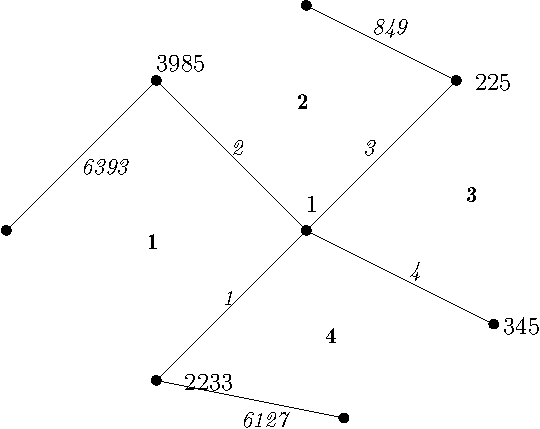
\includegraphics{Figures/dcel.pdf}
  \caption{The particle graph associated with the DCEL of
  	\hyperref[table:dcel]{Table~\ref*{table:dcel}}.
           The dots represent particle centers.  Lines represent the contacts between
           particles.}
           \label{fig:dcel}
\end{figure}
%
\begin{itemize}
\item
Row 3 in an F-file corresponds to contact 3
(see row~3 in Table~\ref{table:dcel}).
\item
Contact 3 is between particle number 1 (\texttt{V1})
and particle number 225 (\texttt{V2})
(i.e., rows 1 and 225 in the corresponding Fb-file).
\item
Void cell 2 (\texttt{F1}) lies on one side of this
contact, and void cell 3 lies on its other side (\texttt{F2}).
%See Section~\ref{sec:ktype2} for a further description of void cells.
\item
Pointer \texttt{P1} (= 4) points to a contact (row 4),
which is also connected to \texttt{V1} (particle number 1)
and lies directly clockwise around \texttt{V1} relative to the 
row 3 contact.
\item
Pointer \texttt{P2} (= 849) points to the contact (row 849)
that is also connected to \texttt{V2} (= particle 225)
and lies clockwise around \texttt{V2} relative
to the third (row 3) contact.
\end{itemize}
The \texttt{hv} data in an Fb-files point to the starting
(header) contact for a
particle 
(\hyperref[sec:f2files]{Section~\ref*{sec:f2files}}).
With this data structure, you will be able to identify all of
the contacts that are connected to an arbitrary particle.
You will also be able to identify all contacts
and particles that lie around the perimeter of
a polygonal void cell.
That is, you can construct both the particle graph and its dual
\cite{Satake:1992a}.
The \texttt{hf} data in an Fd-file points to the starting
(header) contact for a
void cell
(\hyperref[sec:f4files]{Section~\ref*{sec:f4files}}).
\par
The final seven columns in an Fc-file give the following data:
\begin{itemize}
\item
\texttt{branch(1)} and \texttt{branch(2)}:
the horizontal and vertical component of the branch vector that
connects 
the centers of particles \texttt{V1} and \texttt{V2}
(directed toward \texttt{V2}).  Note that the format of these two
fields is \texttt{1pe17.9}.
\item
\texttt{c\_eta(1)} and \texttt{c\_eta(2)}:
the horizontal and vertical components of the unit normal vector, directed
outward from the surface of particle \texttt{V1}
at the contact location.
\item
\texttt{fnold1(1)}:
the magnitude of the 
contact force component that acts normal to the contact surface---a
positive value for compressive contact force.
\item
\texttt{ftold(1)} and \texttt{ftold(2)}:
the horizontal and vertical components of the contact force
tangential to the contact surface.
The force acts upon particle \texttt{V1}.
\item
\texttt{Tstar}:
For Hertz-Mindlin contacts only (\texttt{imodel=5},
(\hyperref[sec:imodel]{Section~\ref*{sec:imodel}}).
See~\citep{Thornton:1988a}.
\end{itemize}
%
\subsubsection{Fc-files for 2D assemblies of non-convex particles}\label{sec:f3files2}
With non-convex particles, such as nobbies,
two particles can have multiple contacts between each other.
The Fc-file gives information identifies the two particles and their
component parts (satellite and central circles) that are touching.
Each line in the Fc-file has format
\texttt{4(i7)},\texttt{2(i8)},\texttt{2(1pe17.9)},
\texttt{i3},\texttt{4(i7,i3,i3)}
and contains the following information:
\begin{itemize}
\item
The first six fields contain \texttt{V1}, \texttt{V2}, \texttt{F1}, \texttt{F2}, \texttt{P1},
and~\texttt{P2}.
These are described in
\hyperref[sec:f3files]{Section~\ref*{sec:f3files}}.
\item
The next two fields contact \texttt{branch(1)} and \texttt{branch(2)}
as described in
\hyperref[sec:f3files]{Section~\ref*{sec:f3files}}.
\item
\texttt{ihit}: the number of contacts between these two particles.
\item
Four triples of integers.  With non-convex particles, such as nobbies,
two particles can have multiple contacts between each other.
Each triple corresponds to one of these contacts.
Each triple is composed of a pointer to
a position within the list of an ``Ff'' file and two identifiers
of the component circles that that are touching (one identifier for
the first particle \texttt{V1}, the other identifier for the
second particle \texttt{V2}).
The identifier is an integer ranging between 0 and \texttt{nobs}:
the zero corresponding to the central circle, numbers 1 and above
corresponding to the satellite circles (arcs).
If a pair of particles has fewer than four contacts, then
zeros will appear in the unused triples.
\end{itemize}
%
\subsubsection{Fd-files for 2D assemblies}\label{sec:f4files}
The lines of this file contain a single integer
in \texttt{i7} format.  The \texttt{hv} integer on 
each line is a pointer to the DCEL for a single void cell
(\hyperref[sec:f3files]{Section~\ref*{sec:f3files}}).
The lines are given in order (for example,
line 14 gives the \texttt{hv} value for void cell number 14).
%
\subsubsection{Ff-files for 2D assemblies}\label{sec:f6files2d}
These files are only created for non-convex particles, such
as nobbies.
Each line in this file gives information on a single contact.
Note that a pair of particles can share multiple contacts.
As described in 
\hyperref[sec:f3files2]{Section~\ref*{sec:f3files2}},
each pair of contacting particles will be represented with a 
single line in an Fc-file.
For non-convex particles, the Fc-file will identify the two particles
(the locations of these particles are given in the Fb-file), 
the branch vector between the particles' centers, 
number of contacts between the two particles,
and triple-integers that identify each of these contacts.
The first integer in a triple points to a line in the Ff-file.
The contents of the Ff-file depends on the contacts'
displacement-force model (\texttt{imodel},
\hyperref[sec:imodel]{Section~\ref*{sec:imodel}}.
%
\par
For nobby particles with a linear-frictional contact
model (\texttt{imodel=0}), 
this line has format \texttt{4(1pe17.9)}
and contains the following information about the contact:
\begin{itemize}
\item
The two components of the contact's normal vector (directed outward
from the first particle, \texttt{V1}).
\item
The normal force (compression is positive).
\item
The three components of the contact's tangential force
(acting upon the first particle, \texttt{V1}).
\end{itemize}
%
\par
For nobby particles with a simple Hertz-Mindlin
model (\texttt{imodel=5}), 
this line has format \texttt{5(1pe17.9)}
and contains the following information about the contact:
\begin{itemize}
\item
The two components of the contact's normal vector (directed outward
from the first particle, \texttt{V1}).
\item
The normal force (compression is positive).
\item
The three components of the contact's tangential force
(acting upon the first particle, \texttt{V1}).
\item
\texttt{Tstar}.
\end{itemize}
%
\par
For nobby particles with the J\"{a}ger\ contact
model (\texttt{imodel=6}), 
this line has format \texttt{7(1pe17.9)}
and contains the following information about the contact:
\begin{itemize}
\item
The two components of the contact's normal vector (directed outward
from the first particle, \texttt{V1}).
\item
The normal force (compression is positive).
\item
The three components of the contact's tangential force
(acting upon the first particle, \texttt{V1}).
\end{itemize}
%
\subsection{F-files for 3D assemblies}\label{sec:ffiles3d}
Four F-files are created together
(\hyperref[table:ffiles]{Table~\ref*{table:ffiles}},
(Table~\ref{table:ffiles}),
and they are described in the following three subsections:
Fa-files
(\hyperref[sec:f1files3d]{Section~\ref*{sec:f1files3d}}),
Fb-files (\hyperref[sec:f2files3d]{Section~\ref*{sec:f2files3d}}),
Fc-files (\hyperref[sec:f3files3d]{Section~\ref*{sec:f3files3d}}),
and Ff-files (\hyperref[sec:f6files3d]{Section~\ref*{sec:f6files3d}}).

\subsubsection{Fa-files for 3D assemblies}\label{sec:f1files3d}
Same data as with 2D assemblies
(\hyperref[sec:f1files]{Section~\ref*{sec:f1files}}).
%
\subsubsection{Fb-files for 3D assemblies}\label{sec:f2files3d}
These files contain information on the size and position of each particle.
Each line gives data for a single particle, with the
lines arranged by particle number (line number 3 in the file is 
for particle~3).
\par
For 3D assemblies of spheres,
the format of each line is \texttt{4(1pe17.9),3(1pe18.9e3)}, with
the following fields 
for each sphere:\\
\begin{center}
\begin{tabular}{lp{3.5in}}
Field 1 & radius \\
Field 2 & $x_{1}$ position of the particle center\\
Field 3 & $x_{2}$ position of the particle center\\
Field 4 & $x_{3}$ position of the particle center\\
Field 5 & $\theta_{1}$ angular orientation of the particle (radians)\\
Field 6 & $\theta_{2}$ angular orientation of the particle (radians)\\
Field 7 & $\theta_{3}$ angular orientation of the particle (radians)
\end{tabular}
\end{center}
\par
For 3D assemblies of ovoids,
the format of each line is \texttt{7(1pe17.9),3(1pe18.9e3)}, with
the following fields
for each ovoid:\\
\begin{center}
\begin{tabular}{lp{3.5in}}
Field 1 & transverse (revolved) half width
(\hyperref[sec:ovoid_data]{Section~\ref*{sec:ovoid_data}})\\
Field 2 & aspect ratio:  axial height / transverse width \\
Field 3 & $x_{1}$ position of the particle center\\
Field 4 & $x_{2}$ position of the particle center\\
Field 5 & $x_{3}$ position of the particle center\\
Field 6 & $\gamma_{1}$ orientation angle (in degrees) of
the particle's axis
(\hyperref[fig:coordinates]{Fig.~\ref*{fig:coordinates}},
\hyperref[sec:ovoid_data]{Section~\ref*{sec:ovoid_data}})\\
Field 7 & $\gamma_{2}$ orientation angle (in degrees) of
the particle's axis
(\hyperref[fig:coordinates]{Fig.~\ref*{fig:coordinates}},
\hyperref[sec:ovoid_data]{Section~\ref*{sec:ovoid_data}})\\
Field 8 & $\theta_{1}$ angular orientation of the particle (radians)\\
Field 9 & $\theta_{2}$ angular orientation of the particle (radians)\\
Field 10 & $\theta_{3}$ angular orientation of the particle (radians)
\end{tabular}
\end{center}
\par
For 3D assemblies of bumpies,
the format of each line is \texttt{4(1pe17.9),4(1pe18.9e3)}, with
the following fields
for each ovoid:\\
\begin{center}
\begin{tabular}{lp{3.5in}}
Field 1 & scaling radius
         (\hyperref[sec:satrad]{Section~\ref*{sec:satrad}}
         and \hyperref[sec:bumpy_data]{Section~\ref*{sec:bumpy_data}})\\
Field 2 & $x_{1}$ position of the particle center\\
Field 3 & $x_{2}$ position of the particle center\\
Field 4 & $x_{3}$ position of the particle center\\
Field 5 & 1st component of the unit orientation quaternion\\
Field 6 & 2nd component of the unit orientation quaternion\\
Field 7 & 3rd component of the unit orientation quaternion\\
Field 8 & 4th component of the unit orientation quaternion
\end{tabular}
\end{center}
%
\subsubsection{Fc-files for 3D assemblies}\label{sec:f3files3d}
Each line in this file gives information on a single contact.
\par
For 3D assemblies of spheres,
the format of each line is \texttt{2i7},\texttt{3(1pe17.9)},
\texttt{4(1pe13.5)}, with
the following fields for each sphere
(with Hertz-Mindlin contacts, the value of \texttt{Tstar} in
format \texttt{1pe13.5} is included at the end of a line):
\begin{itemize}
\item
\texttt{V1} and \texttt{V2}:
the two particle numbers
\item
\texttt{branch(1)}, \texttt{branch(2)}, and \texttt{branch(3)}:
the components of the branch vector that
connects the centers of particle \texttt{V1} and particle \texttt{V2}
(directed toward \texttt{V2}).  Note that the format for these three fields
is \texttt{1pe16.8}.
\item
\texttt{fnold1(1)}:
the magnitude of the contact force 
component that acts normal to the contact surface---a
positive value for compressive forces.
\item
\texttt{ftold(1)}, \texttt{ftold(2)}, and \texttt{ftold(3)}:
the three components of the portion of the contact force
that is tangential to the contact surface.
The force acts upon particle \texttt{V1}.
\item
\texttt{Tstar}:
For Hertz-Mindlin contacts only (\texttt{imodel=5},
\hyperref[sec:imodel]{Section~\ref*{sec:imodel}}).
See~\citep{Thornton:1988a}.
\end{itemize}
%
\par
For 3D assemblies of ovoids,
the format of each line is \texttt{2i7},\texttt{3(1pe17.9)},
\texttt{10(1pe13.5)},with
the following fields
for each ovoid
(with Hertz-Mindlin contacts, the value of \texttt{Tstar} in
format \texttt{1pe13.5} is included at the end of a line):
\begin{itemize}
\item
\texttt{V1} and \texttt{V2}:
the two particle numbers.
\item
\texttt{branch(1)}, \texttt{branch(2)}, and \texttt{branch(3)}:
the components of the branch vector that
connects the centers of particle \texttt{V1} and particle \texttt{V2}
(directed toward \texttt{V2}).  Note that the format for these three fields
is \texttt{1pe17.9}.
\item
\texttt{rx\_i(1)}, \texttt{rx\_i(2)}, and \texttt{rx\_i(3)}:
The components of a vector from the center of particle \texttt{V1}
to the center of the contact point between the two particles.
\item
\texttt{fnold1(1)}:
the magnitude of the contact force
component that acts normal to the contact surface---a
positive value for compressive contact force.
\item
\texttt{ftold(1)}, \texttt{ftold(2)}, and \texttt{ftold(3)}:
the three components of the portion of the contact force
that is tangential to the contact surface.
The tangential force acts upon particle \texttt{V1}.
\item
\texttt{c\_eta(1)}, \texttt{c\_eta(2)}, and \texttt{c\_eta(3)}:
The three components of the unit vector that is the outward normal
of particle \texttt{V1} at the contact point.
\item
\texttt{Tstar}:
For Hertz-Mindlin contacts only (\texttt{imodel=5},
\hyperref[sec:imodel]{Section~\ref*{sec:imodel}}). 
See~\citep{Thornton:1988a}.
\end{itemize}
%
\par
For 3D assemblies of bumpies,
the format of each line is \texttt{2i7},\texttt{3(1pe17.9)},
\texttt{i3},\texttt{6(i7,i3,i3)}, with
the following fields for each bumpy:
\begin{itemize}
\item
\texttt{V1} and \texttt{V2}:
the two particle numbers.
\item
\texttt{branch(1)}, \texttt{branch(2)}, and \texttt{branch(3)}:
the components of the branch vector that
connects the centers of particle \texttt{V1} and particle \texttt{V2}
(directed toward \texttt{V2}).  Note that the format for these three fields
is \texttt{1pe17.9}.
\item
\texttt{ihit}: the number of contacts between these two particles.
\item
Six triples of integers.  With non-convex particles, such as bumpies,
two particles can have multiple contacts between each other.
Each triple corresponds to one of these contacts.
Each triple is composed of a pointer to
a position within the list of an ``Ff'' file and two identifiers 
of the component spheres that that are touching (one identifier for
the first particle \texttt{V1}, the other identifier for the
second particle \texttt{V2}).
The identifier is an integer ranging between 0 and \texttt{nbumps}:
the zero corresponding to the central sphere, numbers 1 and above 
corresponding to the satellite spheres.
\end{itemize}
%
\subsubsection{Ff-files for 3D assemblies}\label{sec:f6files3d}
These files are only created for non-convex particles, such
as bumpies.
Each line in this file gives information on a single contact.
Note that a pair of particles can share multiple contacts.
As described in 
\hyperref[sec:f3files3d]{Section~\ref*{sec:f3files3d}},
Each pair of contacting particles will be represented with a 
single line in an Fc-file.
For non-convex particles, the Fc-file will identify the two particles
(the locations of these particles are given in the Fb-file), 
the branch vector between the particles' centers, 
number of contacts between the two particles,
and triple-integers that identify each of these contacts.
The first integer in a triple points to a line in the Ff-file.
The contents of the Ff-file depends on the contacts'
displacement-force model (\texttt{imodel}, 
\hyperref[sec:imodel]{Section~\ref*{sec:imodel}}).
%
\par
For bumpy particles with a linear-frictional contact
model (\texttt{imodel=0}), 
this line has format \texttt{4(1pe17.9)}
and contains the following information about the contact:
\begin{itemize}
\item
The normal force (compression is positive).
\item
The three components of the contact's tangential force
(acting upon the first particle, \texttt{V1}).
\end{itemize}
%
\par
For bumpy particles with a simple Hertz-Mindlin
model (\texttt{imodel=5}), 
this line has format \texttt{5(1pe17.9)}
and contains the following information about the contact:
\begin{itemize}
\item
The normal force (compression is positive).
\item
The three components of the contact's tangential force
(acting upon the first particle, \texttt{V1}).
\item
\texttt{Tstar}.
\end{itemize}
%
\par
For bumpy particles with the J\"{a}ger\ contact
model (\texttt{imodel=6}), 
this line has format \texttt{7(1pe17.9)}
and contains the following information about the contact:
\begin{itemize}
\item
The three components of the contact's normal vector (directed outward
from the first particle, \texttt{V1}).
\item
The normal force (compression is positive).
\item
The three components of the contact's tangential force
(acting upon the first particle, \texttt{V1}).
\end{itemize}
%
%
\section{Results files for wave propagation simulations}\label{sec:Results}
When \Dempla\ is run in Mode~2,
several files are created with results of a wave propagation
simulation.
These files include the following:
\begin{itemize}
  \item
  A set of \RunFile s,
  one for each RVE, which are created within \Dempla\ (rather
  than by the user).
  Each of these \RunFile s gives the sequence of stress-strain
  control for a single RVE
  (see \hyperref[sec:RunFile]{Section \ref*{sec:RunFile}} about
  \RunFile s,
  particularly the section on
  \hyperref[sec:runfile2]{deformation-stress paths}).
  The files are placed in the \texttt{04\_RunOutput}
  directory (folder), which is inside of the  \BaseName\ directory
  (see \hyperref[item:BaseNameDirectory]{page \pageref*{item:BaseNameDirectory}}).
  The file of a single RVE (i.e., DEM assembly)
  will have the following name:
  \par
  \mbox{%
  \texttt{I}$<$\BaseName\ with suffix$>$\texttt{\_Dempla\_RVE\_}$<$RVE number$>$\texttt{\_}$<$\MotionFile\ name$>$}\\[0.5ex]
  The three parts within ``$<\;>$'' are the three input
  items that are entered at the start of a \Dempla\ wave
  propagation simulation
  (see the \hyperref[par:input]{input description}).
  The RVE number is in the format \texttt{i4.4}, so that the
  fourth RVE from the bottom of the soil column would have
  number 0004.
%
  \item
  A set of files, one for each RVE,
  that gives the screen output that would
  have been created for each RVE.
  This output for an RVE is not actually displayed on the screen,
  but is instead written to a file for viewing later.
  See \hyperref[sec:ScreenOval]{Section \ref*{sec:ScreenOval}} for
  a description of this screen output.
  The screen output files are placed in the \texttt{04\_RunOutput}
  directory (folder), which is inside of the  \BaseName\ directory
  (see \hyperref[item:BaseNameDirectory]{page \pageref*{item:BaseNameDirectory}}).
  The file of a single RVE (i.e., DEM assembly)
  will have the following name:
  \par
  \mbox{%
  	\texttt{S}$<$\BaseName\ with suffix$>$\texttt{\_Dempla\_RVE\_}$<$RVE number$>$\texttt{\_}$<$\MotionFile\ name$>$}\\[0.5ex]
%
  The three parts within ``$<\;>$'' are the three input
  items that are entered at the start of a \Dempla\ wave
  propagation simulation
  (see the \hyperref[par:input]{input description}).
  The RVE number is in the format \texttt{i4.4}, so that the
  fourth RVE from the bottom of the soil column would have
  number 0004.
%
  \item
  A set of output \AFile s and \BFile s, one for each RVE.
  These files are only created if the
  \hyperref[sec:iABfile]{\texttt{iABfile} parameter} is set to 1
  in the simulation's
  \hyperref[sec:GFiles]{\GFile}.
  The files are placed in the \texttt{04\_RunOutput}
  directory (folder), which is inside of the  \BaseName\ directory
  (see \hyperref[item:BaseNameDirectory]{page \pageref*{item:BaseNameDirectory}}).
  The files of a single RVE (i.e., DEM assembly)
  will have the following names:
  \par
  \mbox{%
  	\texttt{B}$<$\BaseName\ with suffix$>$\texttt{\_Dempla\_RVE\_}$<$RVE number$>$\texttt{\_}$<$\MotionFile\ name$>$}\\[0.5ex]
  \mbox{%
  \texttt{A}$<$\BaseName\ with suffix$>$\texttt{\_Dempla\_RVE\_}$<$RVE number$>$\texttt{\_}$<$\MotionFile\ name$>$}\texttt{.txt}\\[0.5ex]
%
  The three parts within ``$<\;>$'' are the three input
  items that are entered at the start of a \Dempla\ wave
  propagation simulation
  (see the \hyperref[par:input]{input description}).
  The RVE number is in the format \texttt{i4.4}, so that the
  fourth RVE from the bottom of the soil column would have
  number 0004.
%
  \item
  A set of ``\texttt{Results}'' files.
  These \ResultsFile s will likely be the most useful ones for analyzing
  the results of \Dempla\ Mode~2 simulations.
  Each file gives a single type of output (stress, pore pressure,
  saturation, etc.) for all of the RVEs or nodes during the full
  duration of the simulation.
  Each file is arranged in rows, with each row usually giving the
  particular result for all of the RVEs (or nodes) at a single
  time step during the simulation.
  \par
  The \ResultsFile s are placed in the \texttt{04\_RunOutput}
  directory (folder), which is inside of the  \BaseName\ directory
  (see \hyperref[item:BaseNameDirectory]{page \pageref*{item:BaseNameDirectory}}).
  The files of a simulation have the following names:
  \par
  \mbox{%
  	\texttt{Results\_}$<$Type$>$\texttt{\_}$<$\BaseName\ with suffix$>$\texttt{\_Dempla\_RVE\_}$<$RVE number$>$ $\ldots$}\\
  \mbox{\quad%
  	\texttt{\_}$<$\MotionFile\ name$>$\texttt{.txt}}\\[0.5ex]
  %
  The $<$Type$>$ specifier is described below and in
  \hyperref[table:ResultsFile]{Table \ref*{table:ResultsFile}}.
  The three parts within ``$<\;>$'' are the three input
  items that are entered at the start of a \Dempla\ wave
  propagation simulation
  (see the \hyperref[par:input]{input description}).
  The RVE number is in the format \texttt{i4.4}, so that the
  fourth RVE from the bottom of the soil column would have
  number 0004.
  \par
  A Mode~2 simulation will create 23 of
  \ResultsFile s, each with the type of data given in
  \hyperref[table:ResultsFile]{Table \ref*{table:ResultsFile}}.
  \begin{table}
  	\centering
    \caption{Contents of various \ResultsFile s for Mode~2
             simulations of wave propagation.
             \label{table:ResultsFile}}
    \begin{tabular}{lcccp{5cm}}
      \hline
      Type & Location & Columns & Format & Description\\
      \hline
      \texttt{u\_1} & Nodes & $N+1$ & \texttt{1pe18.10} &
        Displacement, $u_{1}$\\
      \texttt{u\_2} & Nodes & $N+1$ & \texttt{1pe18.10} &
        Displacement, $u_{2}$\\
      \texttt{u\_3} & Nodes & $N+1$ & \texttt{1pe18.10} &
        Displacement, $u_{3}$\\
      \texttt{s\_11} & RVEs & $N$ & \texttt{1pe14.6} &
        Total normal stress, $\sigma_{11}$\\
      \texttt{s\_12} & RVEs & $N$ & \texttt{1pe14.6} &
        Shear stress,  $\sigma_{12}$\\
      \texttt{s\_13} & RVEs & $N$ & \texttt{1pe14.6} &
        Shear stress,  $\sigma_{13}$\\
      \texttt{s\_22} & RVEs & $N$ & \texttt{1pe14.6} &
        Total normal stress, $\sigma_{22}$\\
      \texttt{s\_23} & RVEs & $N$ & \texttt{1pe14.6} &
        Shear stress,  $\sigma_{23}$\\
      \texttt{s\_33} & RVEs & $N$ & \texttt{1pe14.6} &
        Total normal stress, $\sigma_{33}$\\
      \texttt{w} & Nodes & $N+1$ & \texttt{1pe18.10} &
        Pore fluid displacement in $x_{3}$ direction\\
      \texttt{p} & RVEs & $N$ & \texttt{1pe14.6} &
        Pore fluid pressure, $p$\\
      \texttt{rho\_soil} & Nodes & $N+1$ & \texttt{1pe14.6} &
        Total soil density, $\rho$\\
      \texttt{rho\_fluid} & Nodes & $N+1$ & \texttt{1pe14.6} &
        Total fluid density, $\rho_{\text{f}}$\\
      \texttt{Porosity} & Nodes & $N+1$ & \texttt{1pe14.6} &
        Soil porosity, $n$\\
      \texttt{kperm} & Nodes & $N+1$ & \texttt{1pe14.6} &
        Soil permeability, $k$\\
      \texttt{sat} & Nodes & $N+1$ & \texttt{1pe17.9} &
        Soil saturation, $S$\\
      \texttt{water}& $\ast$ & & \texttt{1pe17.9} &
        Water depth and height from base, $x_{3}$\\
      \texttt{time} & $\dagger$ & & \texttt{1pe17.9} &
        Time from start of \MotionFile\ motion\\
      \texttt{I} & RVEs & $N$ & \texttt{1pe17.9} &
        Inertia number of DEM assembly\\
      \texttt{kn} & RVEs & $N$ & \texttt{1pe17.9} &
        Avg. contact stiffness $k_\text{n}$\\
      \texttt{chi} & RVEs & $N$ & \texttt{1pe17.9} &
        Force imbalance in RVE\\
      \texttt{mass} & RVEs & $N$ & \texttt{1pe17.9} &
        Avg. particle mass in RVE\\
      \texttt{steps} & RVEs & $N$ & \texttt{1pe17.9} &
        Number of DEM steps in a \Dempla\ step $\Delta t$\\
      \hline
      \multicolumn{5}{l}{%
        $\ast$ Two columns: water depth from surface,
        and height from base $x_{3}$} \\
      \multicolumn{5}{l}{%
        $\dagger$ One column: time since the start of the
        simulation (the beginning of the \MotionFile )} \\
      \hline
    \end{tabular}
  \end{table}
%
  All \ResultsFile s begin with five lines, each with a single
  item of data:
%
  \begin{itemize}
    \item
      \texttt{iResultsType} (format \texttt{i8}):
      An indicator of the number of columns that
      each output row will contain.
      This information will help in reading the
      \ResultsFile\ during post-processing with
      programs such as Octave.
      \begin{itemize}
        \item
          \texttt{iResultsType = 0}:
          each row contains \texttt{nRVEs}, $N$,
          data items.
       \item
         \texttt{iResultsType = 1}:
         each row contains \texttt{nRVEs+1}, $N+1$,
         data items.
       \item
          \texttt{iResultsType = 2}:
          each row contains one data item.
        \item
          \texttt{iResultsType = 3}:
          each row contains two data items.
      \end{itemize}
    \item
      \texttt{nRVEs} (format \texttt{i8}): 
      the number of RVEs (DEM assemblies) $N$ in the soil column.
      The value of \texttt{nRVEs} is given as input in
      a \GFile\ (see
      \hyperref[sec:nRVEs]{Section \ref*{sec:nRVEs}}).
    \item
      \texttt{dt\_ref} (format \texttt{1pe21.14}): 
      the time step $\Delta t$ for the Mode~2
      wave propagation simulation.
      Note that this time step applies to the period defined
      by the \MotionFile , and a scaled time step can apply during
      post-shaking consolidation.
    \item
      \texttt{dx\_rve} (format \texttt{1pe21.14}):
      the initial spacing $\Delta x$ of the
      nodes (and RVEs) within the soil column.
    \item
      \texttt{nDempla\_out} (format \texttt{i8}):
      the number of time steps $\Delta t$
      between output lines in the \ResultsFile .
      The value of \texttt{nRVEs} is given as input in
      a \GFile\ (see
      \hyperref[sec:nDemplaout]{Section \ref*{sec:nDemplaout}}).
  \end{itemize}
%
\end{itemize}
%
%
\section{Screen output from \Dempla}\label{sec:ScreenOval}
As a simulation is running, information is printed to the screen, which
can help to monitor the performance of the run.
This information can, of course, 
alternatively be redirected from the screen 
to a file.
The following is an example of the introductory information that might
appear on the screen at the beginning of a simulation:
\par
\footnotesize
\begin{verbatim}
Program OVAL:  version            oval-0.5.41.f
c Matthew R. Kuhn 2001, Licensed under the GPL, version 2

The program was compiled under the following parameters:
   1) 2D or 3D problems. (mdim1=3)
   2) Circular, spherical, elliptical, oval, and ovoid particles. (mpiece=4*mp)
   3) A maximum of 10020 particles. (mp)
Errors will occur if your input data is otherwise (but you can always make
changes to the common-0.5.41 file and recompile).
  
  Name of the RunFile:
LoadComp                 <-- your input here
  Name of the StartFile:
Dsphere_1800             <-- your input here
  
 **** Warning ****.
 * The input value of rho was 0.
 * A mass will be automatically assigned.
  
 **** Warning ****.
 * The input value of dt was 0.
 * A time step will be automatically assigned.

  Your time step is:                1.00000E+00
  The maximum advised time step is: 1.25000E+00

  The assigned particle mass is:    9.76563E+00

  Spherical, 3D particles

  Number of particles     =    1800
  Initial void ratio      =  0.535828
  Initial solids fraction =  0.651115
  Initial porosity        =  0.348885
  Volume of the cell      =  2.248245E+03

  Initial number of contacts       =    5130
  Average ratio of overlap/diameter =  3.186E-04
\end{verbatim}
\normalsize
\par
In this example, the names of the two input files are \texttt{Load1}
and \texttt{Dcircls\_1002}.
The introductory information is followed by a table of diagnostic
information that is periodically updated at the interval \texttt{ipts}, as
specified in the \textsf{RunFile} (Section~\ref{sec:ipts}).
This table will look something like the following:
\par
\footnotesize
\label{verb:screen2}
\begin{verbatim}
Some diagnostic information during this run:
iout    timer istep nupd  ipt2 xloops   chi1      chi2       psi    sweep
   0  0.0000E+00  1    1  18108   1.0  0.00E+00  0.00E+00  0.00E+00  0.00
   1  2.0000E+00  1    1  18108  21.5  1.10E-02  7.73E-03  0.00E+00  0.00
   2  4.0000E+00  1    1  18108   3.0  9.81E-03  7.04E-03  0.00E+00  0.00
   3  6.0000E+00  1    1  18108   3.0  8.79E-03  6.34E-03  0.00E+00  0.00
   4  8.0000E+00  1    1  18108   3.0  7.98E-03  5.74E-03  0.00E+00  0.00
   5  1.0000E+01  2    1  18108   3.0  7.14E-03  5.15E-03  0.00E+00  0.00
   6  5.8000E+01  2    2  18109   2.9  2.42E-03  1.77E-03  3.68E-06  0.00
   7  1.0800E+02  2    2  18109   3.0  3.55E-04  3.77E-04  1.39E-06  0.00
   8  1.5800E+02  2    3  18109   3.0  2.68E-04  3.38E-04  1.17E-06  0.00
\end{verbatim}
\normalsize
Most items in the table were described in
\hyperref[sec:bfile2d]{Section~\ref*{sec:bfile2d}}.
The integer \texttt{istep} is the current
deformation-stress segment
(from the \textsf{RunFile},
\hyperref[sec:runfile2]{Section~\ref*{sec:runfile2}}.
The integer \texttt{nupdat} is the number of near-neighbor searches that
have been performed
(see \hyperref[sec:runfile2]{Section~\ref*{sec:runfile2}}).
The integer \texttt{ipt2} is the current length of the near-neighbor
linked list
(\hyperref[sec:search]{Section~\ref*{sec:search}}).
The value \texttt{xloops} is the average number of iteration loops
(time steps) per deformation step.  When \texttt{algori=1}, then
\texttt{xloops} will always be one.
The values \texttt{}, \texttt{}, and \texttt{} indicate the 
numeric performance of the run
(see Sections~\hyperref[sec:chi1]{\ref*{sec:chi1}},
\hyperref[sec:chi2]{\ref*{sec:chi2}},
and~\hyperref[sec:psi]{\ref*{sec:psi}}
and the other sections referenced from there).
The value \texttt{sweep} is the average number of iterations per
torus-torus contact when ovoids are being used.
%
%
\section{Sample assemblies for \Dempla}\label{sec:samples}
You can download sample \textsf{StartFile} assemblies
from the GitHub repository, 
which are given in a D-file (text) format.
%from the web site given on page~\pageref{page:WebSite}.
%The sample \StartFile s should be located in your \texttt{oval}
%directory in 
%\begin{verbatim}
%    samples/startfiles
%\end{verbatim}
The primary attributes of these assemblies 
are shown in
\hyperref[table:assemblies]{Table~\ref*{table:assemblies}}.
%
\begin{table}
\centering
\begin{tabular}{lccccc}
\hline
\hline
          & Particle & No. of & Void  & Coord. & Dimensionless \\
File Name &   Type   & Particles & Ratio &   Number$^{5}$    &  Overlap      \\
\hline
\texttt{Dcircls\_1002\_2}$^{1}$&circles&1002&0.18042 &3.820 & 3.10$\times10^{-4}$\\
\texttt{Dcircls\_4008\_2}$^{1}$&circles&4008&0.17911 &3.813 & 3.19$\times10^{-4}$\\
\texttt{Dovals\_1002\_1d}      &ovals  &1002&0.18382 &3.784 & 2.32$\times10^{-4}$\\
\texttt{Dovals\_1002\_2d}      &ovals  &1002&0.12890 &4.880 & 1.58$\times10^{-4}$\\
\texttt{Dovals\_4008\_1d}      &ovals  &4008&0.18479 &3.777 & 2.10$\times10^{-4}$\\
\texttt{Dovals\_4008\_2d}      &ovals  &4008&0.12788 &4.733 & 1.72$\times10^{-4}$\\
\texttt{Dsphere\_1800}         &spheres&1800&0.53583 &5.700 & 3.19$\times10^{-4}$\\
\texttt{DOblate\_1800}$^{2}$   &ovoids &1800&0.41520 &8.214 & 1.65$\times10^{-4}$\\
\texttt{DProlate\_1800}$^{3}$  &ovoids &1800&0.41223 &8.438 & 2.01$\times10^{-4}$\\
\texttt{DObProlate\_1800}$^{4}$&ovoids &1800&0.41367 &8.351 & 2.01$\times10^{-4}$\\
\hline
\multicolumn{6}{l}{\parbox{4.80in}{%
$^{1}$The assemblies \texttt{Dcircls\_1002} and 
 \texttt{Dcircls\_4008} in \Oval\ version \texttt{0.4.0} have been
replaced.  These older assemblies were slightly anisotropic.}}\\
\multicolumn{6}{l}{\parbox{4.80in}{%
$^{2} $Oblate ovoids with randomly assigned aspect ratios.  
The aspect ratio is uniformly distributed between 0.65 and 1.00.%
}}\\
\multicolumn{6}{l}{\parbox{4.80in}{%
$^{3} $Prolate ovoids with randomly assigned aspect ratios.
The aspect ratio is uniformly distributed between 1.00 and 1.60.%
}}\\
\multicolumn{6}{l}{\parbox{4.80in}{%
$^{4} $A combination of oblate and prolate ovoids with 
randomly assigned aspect ratios.
The aspect ratio is uniformly distributed between 0.65 and 1.60.%
}}\\
\multicolumn{6}{l}{\parbox{4.80in}{%
$^{5} $The coordination number is computed as twice the number of contacts
divided by the number of particles.
}}\\
\hline
\hline
\end{tabular}
\caption{Attributes of several sample assemblies}
\label{table:assemblies}
\end{table}
Each assembly is roughly square (or cubical)
and with an isotropic fabric.
They were created by isotropically compressing a sparse assembly with
friction turned off.
\par
The assemblies contain a range of particles sizes.
The dimensions of the particles and the entire assemblies have
been scaled so that the mean particle size 
$D_{50}$ in each assembly is 1.00.
(\label{page:d50}Here, 
we speak of the mean particle size $D_{50}$ in the usual sense
of geotechnical engineering:  a ``median'' diameter that partitions
the assembly into two sets of particles, so that each set has an equal
cumulative mass.)
A density plot (normalized histogram) of 
particle radii for both 2D and 3D assemblies is shown
in \hyperref[fig:radii]{Fig.~\ref*{fig:radii}}.
%
\begin{figure}
\centering
\subfigure[2D assemblies]
{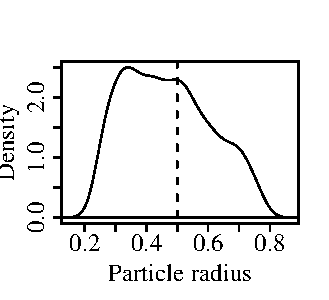
\includegraphics{Figures/radius}}%
\subfigure[3D assemblies]
{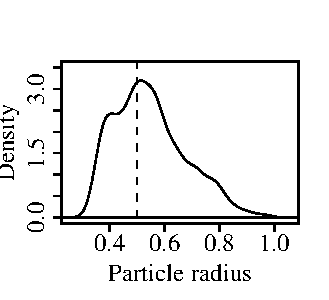
\includegraphics{Figures/radius3d}}%
\caption{Histograms of particle radii for 2D and 3D assemblies}
\label{fig:radii}
\end{figure}
The histogram is centered on the median size $0.50D_{50}$.
In Fig.~\ref{fig:radii}a, the radii of non-circular 2D particles 
refers to their mean radii, $(\mathrm{Height} + \mathrm{Width})/4$
(\hyperref[fig:orientation_angle]{Fig.~\ref*{fig:orientation_angle}},
\hyperref[sec:StartFile2]{Section~\ref*{sec:StartFile2}}).
In \hyperref[fig:radii]{Fig.~\ref*{fig:radii}}b,
the radii of non-spherical 3D particles
refers to their mean radii, $(\mathrm{Height} + 2\cdot\mathrm{Width})/6$
The distribution of aspect ratios for oval and ovoid assemblies
are described in the footnotes of
\hyperref[table:assemblies]{Table~\ref*{table:assemblies}}.
\par
The void ratio is a measure of the packing density of 
a granular assembly 
(\hyperref[table:assemblies]{Table~\ref*{table:assemblies}}).
The assemblies of circles, spheres, and ovoids are fairly dense.
Both loose and dense assemblies of ovals are provided.
The coordination numbers shown in
\hyperref[table:assemblies]{Table~\ref*{table:assemblies}}
are computed as
twice the number of contacts divided by the number of particles.
\par
Among the attributes listed in
\hyperref[table:assemblies]{Table~\ref*{table:assemblies}},
the dimensionless overlap probably has the greatest effect on
the speed and performance of a simulation.
The dimensionless overlaps, which are quite small, were computed
by dividing the average overlap at the particle contacts by the
mean particle size, $D_{50}$.
Small overlaps more closely resemble those in real 
granular materials, which are often composed of hard granules.
During simulations, however, small overlaps
require slower deformation rates to assure the near quasi-static
progression of particle rearrangements.
\par
In addition to the files in
\hyperref[table:assemblies]{Table~\ref*{table:assemblies}},
the website includes a directory 
\texttt{samples/startfiles/Series\_circls\_1002/}
that contains 100 assemblies of 1002 circular particles.
The particle size distribution in each assembly is the same as that of
\texttt{Dcircls\_1002\_2} in
\hyperref[table:assemblies]{Table~\ref*{table:assemblies}}
and \hyperref[fig:radii]{Fig.~\ref*{fig:radii}}a.
Each assembly has exactly the same particle sizes and the same void 
ratio (=0.174257), but the assemblies have different particle arrangements.
As a result of this difference, the files will have modest differences
in the number of contact, dimensionless overlap, and initial stress.
The assemblies were constructed with the same process, but the
the particle radii were shuffled among the particles before
the diffuse assembly was compacted.
%
%
%
\section{Example simulations}\label{sec:examples}
%
\subsection{Mode~1 simulation of monotonic undrained triaxial compression of unsaturated sand}\label{sec:CIUCmono}
\subsubsection{Introduction}\label{sec:CIUCmono1}
This example is described in the author's paper \cite{Kuhn:2020a},
in Sections~3 and~3.2, with results depicted
in Fig.~4a of that paper.
All of the files for the simulation
are in the GitHub folder
\texttt{examples/CIUC\_pq\_unsat\_loose}.
The simulation is of a loose Toyoura Sand 
at a relative density of about 30\%.
The sand is consolidated to an isotropic stress
of 100kPa.
At this stress, the water saturation is 95\%.
The water pressure (back pressure) is increased
to 270kPa while maintaining an effective stress
of 100kPa.
This achieves a 99.9\% saturation
(in separate simulations, discussed in Section~3.1
of the paper, the B-value was 0.42).
The assembly is then monotonically loaded with undrained triaxial
compression while maintaining constant total stress
in the transverse directions.
\par
In \hyperref[sec:CIUCcyclic]{Section~\ref*{sec:CIUCcyclic}},
a similar example is described,
but for a cyclic CIUC test with an amplitude
of 30kPa.
\par
The input \RunFile\ and \StartFile\ are described
in the next section.
As background, the following is a summary of
Section~3 of the paper \cite{Kuhn:2020a}.
%
\par
DEM simulations were conducted to illustrate poroelastic
effects in undrained loading.
Several DEM assemblies were
created with different densities.
Only the simulation with a single assembly is included
in the GitHub examples.
The assemblies were
composed of 10,600 sphere-clusters
within a cubical box, with
characteristics that
were intended to approximate Toyoura Sand.
The particle sizes had a narrow range
(uniformity coefficient $C_{\text{u}}=1.9$)
and a median size D\textsubscript{50} of 0.19~mm.
Because the distribution of particle sizes will affect the bulk properties
of a soil, the sizes of the DEM particles were selected to
approximate the size distribution of Toyoura Sand.
Rather than using spherical particles, each particle was
a composite cluster of seven spheres (see \cite{Kuhn:2014c}).
The complexity of these non-convex clusters
produces assemblies with a more realistic void ratio,
bulk strength, and bulk stiffness.
These characteristics approximate those of
Toyoura Sand, an achievement that is not possible with simple assemblies
of spheres, as sphere assemblies are denser, weaker, and softer than
most sands.
Recently, the use of rotational springs at the contacts has been
proposed as
an expedient approach that uses spheres to produce a greater bulk strength
(for example, \cite{Huang:2017a}).
Neither sphere particles nor
rotational springs were used in the current study,
due to the difficulty of achieving realistic results
for the all three characteristics~--- void ratio,
strength, and stiffness~---
even by manipulating the rotational resistance. 
\par
A series of 29 assemblies was created with 
an isotropic fabric and a range of densities,
with void ratios of 0.596 to 0.984,
roughly the $e_{\text{min}}$
and $e_{\text{max}}$ of Toyoura Sand.
The 25 densest assemblies were created by compacting
the same sparse assembly of 10,600 particles:
a diffuse assembly with a solid fraction of 0.0274 and void
ratio of 35.5.
To simplify the compaction process, we began with particles
having a mean diameter of $D_{50}$ of 1.0 units and linear-frictional
contacts with a unit spring stiffness (the particles' sizes
would later be scaled and a more realistic contact model used,
as explained below).
In other studies,
DEM assemblies are often
compacted from such diffuse assemblies by assigning a
small friction coefficient to the contacts,
but we found that these measures could not produce assemblies as loose
as the loosest Toyoura Sand.
To produce more realistic densities,
we used a friction coefficient of zero and included a
long-range attractive force between particles that was engaged
at inter-particle separations of $0.10 D_{50}$ and nearer.
This measure promoted the agglomeration of particles during
the initial compaction and produced a loose assembly:
a single assembly with a void ratio of 0.985.
After producing this assembly, the attractive mechanism
was removed from the contacts and the particles' sizes were
scaled to those of Toyoura Sand, and further compaction
was then performed with a linear-frictional contact model.
Assemblies with a range of densities were created from this
single initial assembly by using a range of
friction coefficients (from 0.05 to 0.45):
25~assemblies were created with void ratios of 0.596 to 0.941.
To create the four loosest assemblies, with void ratios of 0.950 to 0.984,
we removing 1\% to 4\% of the
particles, randomly chosen, from the one assembly with a void ratio
of 0.941, in the manner of \cite{Nguyen:2018a}.
By removing a progressively larger number of particles from
an already loose assembly,
the void ratio was progressively increased with the four loosest
assemblies, while roughly preserving the arrangements of the remaining particles.
We noted, however, that although these four assemblies had larger void ratios
as a consequence of the randomly dispersed large voids produced by the
removal of particles,
their undrained strengths were not significantly reduced by this
particle-removal process,
indicating that subtle fabric effects (other than density) are
active in affecting undrained behavior.
\par
The final cubic assemblies had dimensions in the range of 2.9~mm to 3.2~mm
for the densest and loosest assemblies, respectively.
The assemblies were bounded on all sides with
periodic boundaries, a technique that produces a homogeneous fabric without
the disruptive influence of boundary platens.
\par 
For the simulations with these assemblies,
we used a contact mechanism
that was more realistic than simple linear springs.
The particles were assigned elastic properties that
approximated those of quartz,
with shear modulus $G_{\text{s}}=29$~GPa,
Poisson coefficient $\nu_{\text{s}}=0.15$,
and bulk modulus $K_{\text{s}}=32$~GPa \citep{Pabst:2013a}.
Because the evolution of water pressure during undrained
loading depends upon the bulk stiffness of the soil skeleton
and because this stiffness changes during loading,
it is essential to use a realistic contact model.
\par
A Hertzian Cattaneo--Mindlin model was used for the contacts,
which was implemented with the J\"{a}ger algorithm
to simulate the complex sequences of contact movements that
occur during cyclic loading paths \citep{Kuhn:2011a}.
The stiffness modulus $G$ of sand is known to depend upon
the effective confining pressure $p$, with $G$ proportional
to $p$ in the form $G\propto p^{\beta}$, with $\beta\approx 0.5$
(for Toyoura Sand, $\beta=0.47$).
Capturing this dependence is important in liquefaction studies,
as the induced excess pore pressure reduces the effective confining pressure
and alters the subsequent behavior.
Simple linear springs do not produce a realistic pressure-dependence
($\beta$ is about 0); the Hertz contact between spheres produces
a $\beta$ of about 0.39; and a Hertz contact between conical
asperities produces a $\beta=0.56$ \citep{Kuhn:2014c}.
For the current study, we adopted a Hertz contact with an
asperity profile intermediate between spherical and conical:
a blunt cone, whose shape is in the form of a power function
with parameters $\alpha$ and $A$
(see \citet{Kuhn:2014c}, with $\alpha=1.5$ and $A_{1.5}=180$).
%
In separate \Dempla\ simulations,
the 29 assemblies exhibited a low-strain shear moduli $G$
that varied with void ratio $e$ and %with mean effective stress
$p$ in a manner that closely approximates Toyoura Sand,
with $G\approx (70\,\text{MPa})(p / 100\,\text{kPa})^{\beta}(2.17-e)^{2}/(1+e)$
and exponent $\beta=0.47$,
when measured at a shear strain of 0.0001 \citep{Hardin:1963a,Iwasaki:1978a}.
The $G_{\text{o}}$ value of 70MPa, the exponent $\beta$,
and the value of 2.17 are
closely approximated by the 29 assemblies.
This agreement between simulations and experiments is not
possible with sphere particles and linear contact springs.
\par
We used an inter-particle friction coefficient of 0.45, 
yielding a bulk strength that was also
similar to Toyoura Sand, 
with a critical state ratio $q/p$ of about 1.22 and a critical
state void ratio of about 0.86 for triaxial
compression loading.
Because both laboratory and DEM results are known
to be sensitive to the loading rate \citep{Hanley:2013a},
we used a consistent strain rate for
all simulations,
with a strain increment of $1\times 10^{-6}$
per time step
(for the quasi-static conditions of this study, in which the particles'
mass densities are scaled, the time-rate is less relevant than the strain
increment, \cite{Suzuki:2014a}).
%
%
\subsubsection{Setup and running the simulation}\label{sec:setupCIUC2}
The GitHub repository contains all of the files for
performing this simulation.
The files for the simulation
are in the GitHub folder
\texttt{examples/CIUC\_pq\_unsat\_loose}.
These are the steps for running \Dempla\ on a Linux system.
%
\begin{enumerate}
	\item
	create the executable file from the fortran source code.
	The steps for doing this with the \textsf{gfortran}
	compiler are described in
	\hyperref[sec:UnixSystems]{Section~\ref*{sec:UnixSystems}}.
	You will need to know the name of the executable
	file and its path.
	\par
	For this simulation the parameter \texttt{mlistJ} should be
	set to 800 in the \texttt{param-dempla.X.X.XX.f} file
	(an \texttt{imodel=9} blunted-cone Jager cont
	was used in the simulation),
	which was sufficient for the simulation.
	\par
	Because this is a Mode~1 simulation of a single
	assembly, there is no advantage of parallelized
	multi-thread running.
	The \texttt{-fopenmp} compile option is not needed
	(see Item~2 on
	\hyperref[item:compile]{page~\pageref*{item:compile}}).
	%
	\item
	Locate the \RunFile\ and \StartFile\ for the
	\Dempla\ simulation.
	These files should be located in the same directory
	in which \Dempla\ is being run.
	If necessary, create links (symlinks, shortcuts, aliases)
	to the \RunFile, \StartFile, and executable
	file in the run directory to these target files
	(in Linux,
	``\texttt{ln -s <path to source file> <given name in current dirctory>}'').
	%
	\item
	now run the \Dempla\ simulation
	by entering the following commands from the main directory
	(one directory above the \BaseName\ directory):
	\begin{verbatim}
		# Change to your path!!!
		PATH_TO_EXECUTABLE="../../source/a.out"
		#
		$PATH_TO_EXECUTABLE << END
		1
		CIUC_pq_unsat_loose_Bvalue_0.42
		DStartFile
		END
	\end{verbatim}
	where \texttt{CIUC\_pq\_unsat\_loose\_Bvalue\_0.42}
	is a link to the \RunFile,
	and \texttt{DStartFile} is a link to the \StartFile.
	The simulation might take several hours to run.
	If you receice the following error message,
	\begin{verbatim}
		Insufficient space in array listJ in subroutin Jager3D
	\end{verbatim}
	then change \texttt{mlistJ} to 800 in the
	\texttt{param-dempla} file of the Fortran source code
	and recompile.
\end{enumerate}
%
%
\subsubsection{Features of the \RunFile}\label{sec:CIUCRunFile}
%
The \RunFile\ is shown in
\hyperref[fig:poro1]{Fig.~\ref*{fig:poro1}}
and
\hyperref[fig:poro2]{Fig.~\ref*{fig:poro2}}.
%
%
\begin{sidewaysfigure}
	\centering\footnotesize
	\begin{verbatim}
Heading with useful information about this particular simulation
       1         : algori   | the algorithm for advancing the particle positions (1 or 2)
       6         : ivers    | add extra input lines (0)
     400         : ncownt   | fequency for updating non-periodic boundaries (0)
       0         : iout(2)  | output files with avg. def. and gradients in layers (0)
       0         : iout(3)  | output files with avg. stresses within layers (0)
       1         : istart   | type of file defining the initial configuration (1 or 3)
       0         : iend     | type of file to be created at end of the run (0, 1, or 3)
       0         : idef     | reference configuration for reporting deformations (0)
     500         : iupdtm   | max. no. of time steps between linked-list updates
       0         : icirct   | compute and regularly update the particle graph (0)
       9         : imodel   | contact model (linear, Hertz, etc.) (0 1, 5, 6, 7, or 9)
       0         : nplatn   | number of additional D-files with boundary particles (0)
       5         : nloop1   | minimum number of iteration loops when algori=2
       0         : iexact   | don't use the same mass for every particle (0 or 1)
       0         : isub     | number of submerged particles (0)
       1         : idamp    | standard or Potyondy/Cundall damping (0, 1, 2, or 3)
       0         : iheat    | temperature-dependent model (0)
       0         : icoef    | enable changing the friction coefficient during a run (0)
       3         : iporo    | poromechanic fluid model (0, 1, 3, or 4)
       0         : ifree(11)| a free input integer.  Placeholder for future versions
       0         : ifree(12)| a free input integer.  Placeholder for future versions
       0         : ifree(13)| a free input integer.  Placeholder for future versions
       0         : ifree(14)| a free input integer.  Placeholder for future versions
       0         : ifree(15)| a free input integer.  Placeholder for future versions
       0         : ifree(16)| a free input integer.  Placeholder for future versions
       0         : ifree(17)| a free input integer.  Placeholder for future versions
       0         : ifree(18)| a free input integer.  Placeholder for future versions
    29.d9        : kn       | normal contact stiffness (force/indentation)
     0.15        : kratio   | ratio of tangential/normal contact stiffnesses
     0.45        : frict    | coefficient of friction at particle contacts
     0.          : frictw   | coefficient of friction between particles and wall
    -1.          : rho      | the mass density of the particle material
     0.250       : sep      | threshold separation during the near-neighbor searches
     0.03        : pcrit(1) | viscosity coefficient for translational body damping
     0.05        : pcrit(2) | viscosity coefficient for rotational body damping
     0.          : pcrit(3) | viscosity coefficient for contact damping
\end{verbatim}

	\caption{An example \textsf{RunFile} -- the upper 38 lines --- for simulating triaxial undrained compression of a quasi-saturated sand specimen.}
	\label{fig:poro1}
\end{sidewaysfigure}
%
\begin{sidewaysfigure}
	\centering\footnotesize
	\begin{verbatim}
     0.64        : xseed    | seed for assigning random initial velocities (when motion=1)
     0.          : rmsvel   | rms initial velocity (when motion=1)
     0.10        : pdif     | parameter for reducing Jager memory demand (when imodel>=6)
     0.          : tmax     | maximum time for the simulation run
   180.0         : A_1      | shape factor for conical contact profile (A_1)
    -1.          : dt       | time increment
     0.          : gravty(1)| gravity in x_1 direction. Depracated. (0.)
     0.          : gravty(2)| gravity in x_2 direction. Depracated. (0.)
     0.          : gravty(3)| gravity in x_3 direction. Depracated. (0.)
     0.          : p_o      | initial fluid pressure of pore liquid relative to atm. pressure
    31.8d9       : K_s      | bulk modulus of grain bodies (when iporo = 1, 3, or 4)
     2.2d9       : K_f      | bulk modulus of pore fluid (when iporo = 1 or 3)
     0.95d0      : S_o      | initial fluid saturation of pore space at p_o (iporo=2,3)
   100.d3        : p_atm    | the reference atmospheric pressure (iporo=2,3)
     0.0187d0    : Hcc      | Henry's coefficient of pore liquid/gass (iporo=3)
    72.75d-3     : gamm     | surface tension of pore bubbles (iporo=3)
     0.0001d0    : D_o      | initial bubble diameter at p_o and S_o (iporo=3)
     0.          : N_o      | number/density bubbles per unit initial pore volume(iporo=3)
  2337.d0        : p_vap    | water vapor pressure relative to atm. pressure (iporo=3)
     0.          : p_wcav   | cavitation pressure relative to atm. pressure (iporo=3)
     0.          : rfree(15)| placeholder
     0.          : rfree(16)| placeholder
     0.          : rfree(17)| placeholder
     0.          : rfree(18)| placeholder
     1.5         : palpha   | alpha power in contact profile (when imodel=9)
                                                                                                   imicro
       ************  Deformation-Stress Path Segments  **********             krotat           iflexc |             iplot
   icontp (100000)   (10000)   (1000)    (100)      (10)      (1)                 |            idump  | |ibodyf    ipts2 |
icontr |  rate_11 | rate_22 | rate_33 | rate_12 | rate_13 | rate_23    vrate  igoal   finalv  ipts |  | | |  defdot  |   |
------|-|---------|---------|---------|---------|---------|---------|---------|--|-|---------|----|-|--|-|--|------|----|--|
111000 1  0.000e+0  0.000e+0  0.000e+0  0.000e+0  0.000e+0  0.000e+0  0.000e+0 70 0     5000.  500 0  0 0  0     0.    0  0
111000 1      -25.      -25.      -25.  0.000e+0  0.000e+0  0.000e+0  0.000e+0 11 0  -100000.  100 0  0 0  0     0.    0  0
111000 1  0.000e+0  0.000e+0  0.000e+0  0.000e+0  0.000e+0  0.000e+0  0.000e+0 70 0     1000.  100 0  0 0  0     0.    0  0
111000 1  0.000e+0  0.000e+0  0.000e+0  0.000e+0  0.000e+0  0.000e+0       50. 70 0     5400.   50 0  0 0  0     0.    0  0
111000 1  0.000e+0  0.000e+0  0.000e+0  0.000e+0  0.000e+0  0.000e+0        0. 70 0      500.  100 0  0 0  0     0.    0  0
066000 0 -1.000e-6  0.000e+0  0.000e+0  0.000e+0  0.000e+0  0.000e+0  0.000e+0 70 0      400.   20 0  0 0  0     0.    0  0
066000 0 -1.000e-6  0.000e+0  0.000e+0  0.000e+0  0.000e+0  0.000e+0  0.000e+0 70 0     1000.   50 0  0 0  0     0.    0  0
066000 0 -1.000e-6  0.000e+0  0.000e+0  0.000e+0  0.000e+0  0.000e+0  0.000e+0 70 0    50000.  100 0  0 0  0     0.    0  0
066000 0 -1.000e-6  0.000e+0  0.000e+0  0.000e+0  0.000e+0  0.000e+0  0.000e+0 70 0   250000.  100 0  0 0  0     0.    0  0
\end{verbatim}

	\caption{An example \textsf{RunFile} -- the lower lines --- for simulating triaxial undrained compression of a quasi-saturated sand specimen.}
	\label{fig:poro2}
\end{sidewaysfigure}
%
The \RunFile\ for the simulation
are in the GitHub folder
\texttt{examples/CIUC\_pq\_unsat\_loose},
which is present as a symbolic link to the
source \RunFile\ in the \texttt{RunFiles} folder.
Most of the parameters in this \RunFile\ are
described in the Mode~2 wave propagation simulation of
\hyperref[sec:examplewave3]{Section~\ref*{sec:examplewave3}}.
The friction coefficient \texttt{frict}
(\hyperref[sec:frict]{Section~\ref*{sec:frict}})
and the shape parameters for the blunted cone contact
(\texttt{A\_1} and \texttt{palpha}) were selected 
by conducting a series of separate simulations,
in a trial-and-error manner
(\hyperref[sec:A1]{Section~\ref*{sec:A1}} and
\hyperref[sec:palpha]{Section~\ref*{sec:palpha}}
and the reference \cite{Kuhn:2014c}).
The values of \texttt{A\_1} and \texttt{palpha}
were chosen so that the following results wer
obtained: (1)~the assembly had the
same shear modulus as Toyoura Sand
when the mean stress was 100~kPa,
and (2)~the shear modulus increased with mean stress
with a similar power-law as Toyoura Sand.
The friction coefficient \texttt{frict}
was adjusted with a trial-and-error process,
so that the strength (monotonic and cyclic)
was similar to Toyoura Sand.
In these simulations, a consistent loading rate was used.
Also see the paper \cite{Kuhn:2021a}.
Nite that the initial water saturation
\texttt{S\_o} is 95\%,
and the initial water pressure is atmospheric
(\texttt{p\_o=0.}, \hyperref[sec:po]{Section~\ref*{sec:po}}).
%
\par
Another important aspect of the \RunFile\ are
the values \texttt{rho=-1.} and \texttt{dt=-1.}
(see \hyperref[sec:rho]{Section~\ref*{sec:rho}}
and \hyperref[sec:dt]{Section~\ref*{sec:dt}}).
With these values, there is no need to decide upon
a value of the DEM time step.
The time step is set to 1~second,
and the masses of the particles are adjusted,
so that the simulation will be nearly
quasi-static.
%
\par
%
The deformation-stress control sequence is given
in the final 9 lines of 
\hyperref[fig:poro2]{Fig.~\ref*{fig:poro2}},
and these lines are described belowa:
\begin{enumerate}
\item
The first line is 5000 time-steps of a
quiescent period (\texttt{igoal=70} specifies that that
the period is limited by the number of time steps,
and the value of \texttt{finalv=5000} specifies
the number of steps,
described in
\hyperref[sec:igoal]{Section~\ref*{sec:igoal}} and
\hyperref[sec:finalv]{Section~\ref*{sec:finalv}}).
This quiescent period is needed to allow the
\DFile\ assembly to become equilibrated under the
conditions of the contacts' stiffnesses.
The period is ``quiescent'' because the value
of \texttt{icontr=111000} means that the three normal
effective
stresses are being controlled (the 1's) with
rates of zero (the values of
\texttt{defrat(1)}, or ``rate\_11'' etc.).
See \hyperref[sec:icontr]{Section~\ref*{sec:icontr}} and
\hyperref[sec:defrat]{Section~\ref*{sec:defrat}} for
descriptions of \texttt{icontr} and \texttt{defrat}.
The shearing deformation rates are also zero.
The value \texttt{icontp=1}, meaning that
the pore water pressure is also being controlled
The initial water pressure \texttt{p\_o=0.} is zero
relative to atmospheric pressure,
and the \texttt{defrat(8)=0.} for the first period,
so the water pressure is maintained at zero
relative to atmospheric pressure
(see \hyperref[sec:icontp]{Section~\ref*{sec:icontp}} and
\hyperref[sec:defrat8]{Section~\ref*{sec:defrat8}}
for descriptions
of \texttt{icontp} and \texttt{defrat(8)}).
%
\item
In the second period,
the effective normal stresses are controlled,
the shearing deformations are controlled
(\texttt{icontr=111000}), and their rates are given by
\texttt{defrat}.
In this period, the shear rates are zero
(\texttt{defrat(4)}, \texttt{defrat(5)},
and \texttt{defrat(6)}),
but the effective normal stresses are increased
(negative, greater compression) at 25Pa per time
step~--- isotropic compression
(\texttt{defrat(1)}, \texttt{defrat(2)},
and \texttt{defrat(3)}).
The effecive stresses are to be increased
until the effective stress $\sigma_{11}$
reaches 100,000Pa.
Note that \texttt{igoal=11}: the first "1"
means that a terminal value is given in the $x_{1}$
direction, and the second "1" means that a terminal
value of effective stress
(not deformation or total stress)
is given for the $x_{1}$ direction.
During this period, the, drained conditions are
maintained:
the pore pressure (not water infusion) is maintained
(\texttt{icontp=1}), and the pressure rate
is zero (\texttt{defrat(8)=0.}, i.e. \texttt{vrate}).
Note that the choice of direction of the 25kPa/step depends
on whether the effective stress at the start of the second
period is greater than or less than the target
of -100,000Pa.
In the case of this simulation,
the stress at the end of the first period is
-3,557Pa, so the rate should be -25Pa/step.
If a positive value was given, a runaway simulation
would occur.
%
\item
The third period is similar to the first
period~--- a quiescent period of 1000 time steps.
However, the effective stress is now being maintained
at 100,000Pa.
The water pressure is being maintained at atmospheric pressure.
%
\item
In the fourth period,
we maintain the same effective stresses,
but the pore water pressure (back pressure)
is controlled (\texttt{icontp=1}, meaning drained)
and is increased
at a rate of 50Pa per time step.
The water pressure is increased
for 5400 time steps (\texttt{igoal=70} means that
a specified number of time steps are run,
anf \texttt{finalv=5400}).
This will increase the water pressure to 270,000Pa
above atmospheric pressure.
At the end of the fourth period,
the saturation is 99.939\%.
(A pressure of 283,000 would be required
to achieve full saturation.)
%
\item
The fifth period is another quiescent period,
like the first and third periods.
The fifth period lasts for 500 time steps.
%
\item
The next four periods (periods 6, 7, 8, and 9)
conduct the triaxial undrained compression.
The value \texttt{icontr=066000} means that deformation
is controlled in the $x_{1}$ direction (the first 0),
the total normal stress is controlled
in the $x_{2}$ and $x_{3}$ directions (the second
and third 6's),
and the shearing strains are zero.
The $x_{1}$ deformation rate $\dot{F}_{11}$
is $-1.00\times 10^{-6}$ per time step.
The rates of the $x_{2}$ and $x_{3}$ total stresses
are zero (i.e., constant chamber pressure).
The periods are undrained:
the value of \texttt{icontp=0} means that the inflow
of fluid into the specimen is being controlled;
the \texttt{defrat(8)} (i.e., \texttt{vrate})
of zero means that no fluid
flows into or out of the specimen
(\hyperref[sec:icontp]{Section~\ref*{sec:icontp}}
and \hyperref[sec:defrat8]{Section~\ref*{sec:defrat8}}).
Note that the volume of the specimen can change,
if the air bubbles increase or decrease in size.
The four periods only differ in the frequency
at which the output results are written to
the \AFile\ and \BFile\ (the values of \texttt{ipts},
\hyperref[sec:ipts]{Section~\ref*{sec:ipts}}).
\end{enumerate}
%
%
%
%
\subsection{Mode~1 simulation of cyclic undrained triaxial compression of unsaturated sand}\label{sec:CIUCcyclic}
%
\subsubsection{Introduction}
As with the previous example in
\hyperref[sec:CIUCmono]{Section~\ref*{sec:CIUCmono}},
this example is of an isotropically consolidated
undrained compression test,
but the previous example was of monotonic loading.
The current example is of cyclic loading.
This example is described in the author's paper \cite{Kuhn:2020a},
in Sections~3 and~3.3, with results depicted
in Fig.~5a of that paper.
All of the files for the simulation
are in the GitHub folder
\texttt{examples/CIUC\_Cyclic\_unsat\_loose}.
The simulation is of a loose Toyoura Sand 
at a relative density of about 30\%.
The sand is consolidated to an isotropic stress
of 100kPa.
At this stress, the water saturation is 95\%.
The water pressure (back pressure) is increased
to 270kPa while maintaining an effective stress
of 100kPa.
This achieves a 99.9\% saturation
(in separate simulations, discussed in Section~3.1
of the paper, the B-value was 0.42).
The assembly is then cyclically loaded
with undrained triaxial
compression at an amplitude of 30kPa
while maintaining constant total stress
in the transverse directions.
The specimen fully liquefies.
In figure 5a of the paper \cite{Kuhn:2020a},
shows a line for the B-value of 0.42, which
is the results of six different simulations,
each with a different cyclic amplitude.
This particular simulation has an amplitude
of 30kPa.
%
\par
\hyperref[sec:CIUCmono1]{Section~\ref*{sec:CIUCmono1}}
gives background information about the assembly
preparation and details about the contact model.
We skip repeating this information,
and now describe the setup and running
of the simulation and details about the \RunFile.
Because the same soil is simulated,
the \DFile\ for this simulation is the as that used
in the previous example.
%
%
\subsubsection{Setup and running the simulation}\label{sec:setupCIUC}
The GitHub repository contains all of the files for
performing this simulation.
The files for the simulation
are in the GitHub folder
\texttt{examples/CIUC\_Cyclic\_unsat\_loose}.
These are the steps for running \Dempla\ on a Linux system.
%
\begin{enumerate}
	\item
	create the executable file from the fortran source code.
	The steps for doing this with the \textsf{gfortran}
	compiler are described in
	\hyperref[sec:UnixSystems]{Section~\ref*{sec:UnixSystems}}.
	You will need to know the name of the executable
	file and its path.
	\par
	For this simulation the parameter \texttt{mlistJ} should be
	set to 800 in the \texttt{param-dempla.X.X.XX.f} file
	(an \texttt{imodel=9} blunted-cone Jager cont
	was used in the simulation),
	which was sufficient for the simulation.
	\par
	Because this is a Mode~1 simulation of a single
	assembly, there is no advantage of parallelized
	multi-thread running.
	The \texttt{-fopenmp} compile option is not needed
	(see Item~2 on
	\hyperref[item:compile]{page~\pageref*{item:compile}}).
	%
	\item
	Locate the \RunFile\ and \StartFile\ for the
	\Dempla\ simulation.
	These files should be located in the same directory
	in which \Dempla\ is being run.
	If necessary, create links (symlinks, shortcuts, aliases)
	to the \RunFile, \StartFile, and executable
	file in the run directory to these target files
	(in Linux,
	``\texttt{ln -s <path to source file> <given name in current dirctory>}'').
	%
	\item
	now run the \Dempla\ simulation
	by entering the following commands from the main directory
	(one directory above the \BaseName\ directory):
	\begin{verbatim}
		# Change to your path!!!
		PATH_TO_EXECUTABLE="../../source/a.out"
		#
		$PATH_TO_EXECUTABLE << END
		1
		CIUC_Cyclic_unsat_loose_Bvalue_0.42
		DStartFile
		END
	\end{verbatim}
	where \texttt{CIUC\_pq\_unsat\_loose\_Bvalue\_0.42}
	is a link to the \RunFile,
	and \texttt{DStartFile} is a link to the \StartFile.
	The simulation might take several hours to run.
	If you receice the following error message,
	\begin{verbatim}
		Insufficient space in array listJ in subroutin Jager3D
	\end{verbatim}
	then change \texttt{mlistJ} to 800 in the
	\texttt{param-dempla} file of the Fortran source code
	and recompile.
\end{enumerate}
%
%
\subsubsection{Features of the \RunFile}
%
A part of the \RunFile\ is shown in
\hyperref[fig:poro3]{Fig.~\ref*{fig:poro3}}.
Only the middle portion is shown.
%
\begin{sidewaysfigure}
\centering\footnotesize
\begin{verbatim}
     6.d5        : tmax     | maximum time for the simulation run
   180.0         : A_1      | shape factor for conical contact profile (A_1)
    -1.          : dt       | time increment
     0.          : gravty(1)| gravity in x_1 direction
     0.          : gravty(2)| gravity in x_2 direction
     0.          : gravty(3)| gravity in x_3 direction
     0.          : p_o      | initial fluid pressure of pore liquid
    31.8d9       : K_s      | bulk modulus of grain bodies
     2.2d9       : K_f      | bulk modulus of pore fluid
     0.95d0      : S_o      | initial fluid saturation of pore space at p_o (iporo=2,3)
   100.d3        : p_atm    | the reference atmospheric pressure (iporo=2,3)
     0.0187d0    : Hcc      | Henry's coefficient of pore liquid/gass (iporo=3)
    72.75d-3     : gamm     | surface tension of pore bubbles (iporo=3)
     0.0001d0    : D_o      | initial bubble diameter at p_o and S_o (iporo=3)
     0.          : N_o      | number/density bubbles per unit initial pore volume(iporo=3)
  2337.d0        : p_vap    | water vapor pressure relative to atm. pressure (iporo=3)
     0.          : p_wcav   | cavitation pressure relative to atm. pressure (iporo=3)
     0.          : rfree(15)| placeholder
     0.          : rfree(16)| placeholder
     0.          : rfree(17)| placeholder
     0.          : rfree(18)| placeholder
     1.5         : palpha   | alpha power in contact profile (when imodel=9)
                                                                                                   imicro
       ************  Deformation-Stress Path Segments  **********             krotat           iflexc |             iplot
   icontp (100000)   (10000)   (1000)    (100)      (10)      (1)                 |            idump  | |ibodyf    ipts2 |
icontr |  rate_11 | rate_22 | rate_33 | rate_12 | rate_13 | rate_23    vrate  igoal   finalv  ipts |  | | |  defdot  |   |
------|-|---------|---------|---------|---------|---------|---------|---------|--|-|---------|----|-|--|-|--|------|----|--|
111000 1  0.000e+0  0.000e+0  0.000e+0  0.000e+0  0.000e+0  0.000e+0  0.000e+0 70 0     5000.  500 0  0 0  0     0.    0  0
111000 1      -25.      -25.      -25.  0.000e+0  0.000e+0  0.000e+0  0.000e+0 11 0  -100000.  100 0  0 0  0     0.    0  0
111000 1  0.000e+0  0.000e+0  0.000e+0  0.000e+0  0.000e+0  0.000e+0  0.000e+0 70 0     1000.  100 0  0 0  0     0.    0  0
111000 1  0.000e+0  0.000e+0  0.000e+0  0.000e+0  0.000e+0  0.000e+0       50. 70 0     5400.   50 0  0 0  0     0.    0  0
111000 1  0.000e+0  0.000e+0  0.000e+0  0.000e+0  0.000e+0  0.000e+0        0. 70 0      500.  100 0  0 0  0     0.    0  0
066000 0 -1.000e-6  0.000e+0  0.000e+0  0.000e+0  0.000e+0  0.000e+0  0.000e+0 12 0 -4.00e+05   20 0  0 0  0     0.    0  0
066000 0  1.000e-6 -0.000e+0 -0.000e+0  0.000e+0  0.000e+0  0.000e+0  0.000e+0 12 0 -3.40e+05   20 0  0 0  0     0.    0  0
066000 0 -1.000e-6  0.000e+0  0.000e+0  0.000e+0  0.000e+0  0.000e+0  0.000e+0 12 0 -4.00e+05   20 0  0 0  0     0.    0  0
066000 0  1.000e-6 -0.000e+0 -0.000e+0  0.000e+0  0.000e+0  0.000e+0  0.000e+0 12 0 -3.40e+05   20 0  0 0  0     0.    0  0
066000 0 -1.000e-6  0.000e+0  0.000e+0  0.000e+0  0.000e+0  0.000e+0  0.000e+0 12 0 -4.00e+05   20 0  0 0  0     0.    0  0
\end{verbatim}

\caption{An example \textsf{RunFile} -- the lower lines --- for simulating cyclic triaxial undrained compression of a quasi-saturated sand specimen.}
\label{fig:poro3}
\end{sidewaysfigure}
%
The \RunFile\ for the simulation
is in the GitHub folder
\texttt{examples/CIUC\_Cyclic\_unsat\_loose},
which is present as a symbolic link to the
source \RunFile\ in the \texttt{RunFiles} folder.
Most of the parameters in this \RunFile\ are
described in the Mode~2 simulation of wave propagation in
\hyperref[sec:examplewave3]{Section~\ref*{sec:examplewave3}}
and in the monotonic CIUC simulation of
\hyperref[sec:CIUCRunFile]{Section~\ref*{sec:CIUCRunFile}}.
In this section, we will only describe differences
between the monotonic and cyclic CIUC \RunFile s.
The monotonic loading \RunFile\ is shown in
\hyperref[fig:poro1]{Fig.~\ref*{fig:poro1}}
and \hyperref[fig:poro2]{Fig.~\ref*{fig:poro2}}.
%
\par
An important difference between the monotonic and cyclic
loading \RunFile s is the value of \texttt{t\_max} in
the cyclic file.
A value of 600,000 time steps is given for cyclic
loading.
The cyclic \RunFile\ includes over 100 cycles of
cyclic loading.
The \hyperref[fig:poro3]{Fig.~\ref*{fig:poro3}} only
shows the first 5 lines of this cyclic loading
in the deformation--stress control portion of 
the file (the last 5 lines of the figure).
When running the simulation, you would not know
how many cycles of loading are needed before the
assembly liquefies.
When liquefaction occurs and the specimen fails,
\Dempla\ will run indefinitely, continuing until the
target terminal stress of the
particular deformation--stress period is reached.
The use of \texttt{t\_max} will halt the \Dempla\ run,
so that it does not continue to run indefinitely
(see \hyperref[sec:tmax]{Section~\ref*{sec:tmax}}
for a description of \texttt{t\_max}).
(In older cyclic triaxial laboratory equipment,
the operator would need to stand by, ready
to kill the test, so that the equipment would not
destroy itself when cyclic failure had occurred.)
%
\par
%
In \hyperref[fig:poro3]{Fig.~\ref*{fig:poro3}},
the first five lines of deformation--strain control
are the same as those of 
\hyperref[sec:CIUCRunFile]{Section~\ref*{sec:CIUCRunFile}}:
an initial period of quiescence to allow the 
particles to equilibrate;
an isotropic increase in the effective stress
to 100kPa;
another quiescent period;
an increase of the pore fluid pressure from
atmospheric pressure to 270kPa
above atmospheric pressure;
and another quiescent period.
At this stage,
the total isotropic stress was $-$370kPa,
the water pressure was 270kPa, the
effective stress was $-$100kpa,
and a water saturation was 99.939\%.
\par
The next five lines are the beginning
of cyclic CIUC loading
(there are at least 200 of these lines).
In all of these lines,
\texttt{icontp=0}, meaning that the inflow of fluid is
being controlled.
The value of \texttt{defrat(8)=0.} (i.e., \texttt{vrate}),
meaning that the rate of inflow (as a compressive strain
in the pore fluid) is zero.
Undrained conditions are maintained with
these values of \texttt{icontp} and \texttt{defrat(8)=0}
(see \hyperref[sec:defrat8]{Section~\ref*{sec:defrat8}}).
With these lines, the value of \texttt{defrat(1)} in the
$x_{1}$ direction (i.e., \texttt{rate\_11}) alternates
between \texttt{-1.000e-6} and \texttt{1.000e-6},
meaning that these are changes (per time step) in
the deformation gradient $F_{11}$
(see \hyperref[sec:defrat]{Section~\ref*{sec:defrat}}).
The alternation of strain rate produces the
cyclic loading.
When the rate is \texttt{-1.000e-6},
the value of \texttt{igoal=12}:
the first digit ``1'' means that terminal condition
is related to the $x_{1}$ direction of deformation
or stress, anf the second digit ``2''
means that the terminal condition is a total stress
(i.e., the total stress $\sigma_{11}$,
see \hyperref[sec:igoal]{Section~\ref*{sec:igoal}}).
The value of \texttt{finalv=-4.00e+05},
meaning that this deformation--stress control
period is terminated when the stress becomes $-$400kPa
(remember that the ambient total stress is
$-$400kPa and the $x_1$ \texttt{defrat(1)} is negative).
See \hyperref[sec:finalv]{Section~\ref*{sec:finalv}}
for a description
of \texttt{finalv}.
These lines alternate with lines having
a terminal total stress of $-$340kPa.
Thus, the cyclic amplitude is 30kPa.
%
%
%
\subsection{Mode~2 wave propagation in dry soil column}\label{sec:mode2example}
%
\subsubsection{Introduction}
This example is described in the author's paper \cite{Kuhn:2021a},
in Sections~4 and~4.1.
The simulation is intended to give a realistic simulation
of wave propagation that compares well with a
centrifuge test with Nevada Sand.
The simulation is of a
11~m deposit of dense dry sand at $D_{\text{r}}=$ 101\%
subjected to horizontal shaking
with a seismic motion \cite{Stevens:1999a}.
Although the paper gives the results of a set of three separate
simulations (and centrifuge tests),
only one of the simulations is described here.
%
The set of three centrifuge tests was
performed at the University of California, Davis, on a
homogeneous, level, and dry deposit of
dense sand with $D_{\text{r}}=$ 100\%
\cite{Stevens:1999a}.
The tests were performed on a model of 558~mm depth.
Two tests, including the simulation of this example
were at a lower centrifuge speed
(acceleration 20~g, DKS02\_bb and DKS02\_be),
simulating an 11~m thick deposit;
the third test (not described here),
at a higher speed (acceleration 40~g, DKS02\_bl),
simulated a 22~m thickness.
The centrifuge box was a flexible shear beam,
and in the simulations, the sand's mass was
increased by 24\% to account for the box mass
(e.g., \cite{Elgamal:2005a}). 
Three different seismic motions, taken from the same flight DKS02,
were selected for simulation (only one seismic motion is
used with this example).
The base motions were scaled versions of the 
1989 Loma Prieta SCZ090 record,
available from the Strong-Motion Virtual Data Center \cite{VDC:2021a}.
%used in set~1, and these motions were retrieved directly from data
As was done in \cite{Elgamal:2005a},
the motions at model depth 483~mm
(accelerometer~A17)
were used as input for the simulations. 
The data streams from all instruments are available from
\cite{CGM:2021a}, and the full program is documented by
Stevens et al. \cite{Stevens:1999a}.
%
\subsubsection{Setup and running the simulation}\label{sec:setupwave}
The GitHub repository contains all of the files for
performing this simulation.
These are the steps for running \Dempla\ on a Linux system.
%
\begin{enumerate}
	\item
	create the executable file from the fortran source code.
	The steps for doing this with the \textsf{gfortran}
	compiler are described in
	\hyperref[sec:UnixSystems]{Section~\ref*{sec:UnixSystems}}.
	You will need to know the name of the executable
	file and its path.
	\par
	%
	For this simulation the parameter \texttt{mlistJ} was
	set to 200 in the \texttt{param-dempla.X.X.XX.f} file
	(an \texttt{imodel=9} blunted-cone Jager cont
	was used in the simulation),
	which was sufficient for the simulation.
	\item
	from the main directory (folder) from which you are running the
	simulation, create a link to the directory
	``\texttt{MotionInput}'' that contains
	the \MFile s of motion histories
	(see \hyperref[sec:MFiles]{Section~\ref*{sec:MFiles}}
	for a description of \MFile s).
	For example, if you are using the
	same directory structure as in the github archive, you could run
	the simulation from within the \texttt{examples/} directory.
	Note that
	the \texttt{MotionInput}
	directory is not located inside of \texttt{examples/}, but it
	probably contains a symbolic link
	(symlink, similar to a shortcut in Windows or an Alias in MacOS)
	to the \texttt{MotionInput} 
	directory.
	Create a link commands similar to these:
	%
	\begin{verbatim}
		cd <folder from which you are running the simulation>
		ln -s <path to the MotionInput directory> MotionInput
	\end{verbatim}
	%
	Note: if the directory
	from which you are running the simulation contains
	the actual \texttt{MotionInput} folder,
	then you won't need to create the link.
	\par
	The particular \MFile\ for this simulation is named
	\texttt{Motion\_DKS02\_bb\_A17\_Model},
	and it is included in the github repository.
	Make sure that this file is included in your own
	\texttt{MotionInput} directory.
	%
	\item
	from the same directory (the main directory from which you are running 
	the simulation), create a link to the directory \texttt{RunFiles} that
	contains the \RunFile s (these files give the parameters for running
	the DEM simulations at each RVE, see
	\hyperref[sec:RunFile]{Section~\ref*{sec:RunFile}}).
	\begin{verbatim}
		cd <folder from which you are running the simulation>
		ln -s <path to the RunFiles directory> RunFiles
	\end{verbatim}
	Note: if the directory
	from which you are running the simulation contains
	the actual \texttt{RunFiles} directory,
	then you won't need to create the link.
	%
	\item
	from the same directory
	(the main directory from which you are running 
	the simulation),
	create a link to the directory \texttt{StartFiles} that
	contains the \StartFile s (these files give the parameters for running
	the DEM simulations at each RVE,
	see \hyperref[sec:StartFile1]{Section~\ref*{sec:StartFile1}}).
	\begin{verbatim}
		cd <folder from which you are running the simulation>
		ln -s <path to the StartFiles directory> StartFiles
	\end{verbatim}
	Note: if the directory
	from which you are running the simulation contains
	the actual \texttt{StartFiles} folder,
	then you won't need to create the link.
	%
	\item
	create the directory with the \BaseName\ of the simulation, along with
	three additional directories.
	The \BaseName\ of this particular simulation is 
	\texttt{DKS02\_bb\_B\_mu005\_f040\_A17}:
	\begin{verbatim}
		mkdir DKS02_bb_B_mu005_f040_A17
		mkdir DKS02_bb_B_mu005_f040_A17/02_LayerSetup
		mkdir DKS02_bb_B_mu005_f040_A17/03_RVESetup
		mkdir DKS02_bb_B_mu005_f040_A17/04_RunOutput
	\end{verbatim}
	%
	\item
	create the \GFile\ that gives the conditions of the soil column
	(see \hyperref[sec:GFiles]{Section~\ref*{sec:GFiles}}).
	Place this \GFile inside of the \BaseName\ folder
	(in this example, the folder
	\texttt{DKS02\_bb\_B\_mu005\_f040\_A17}). 
	For this example,
	the \GFile is named
	\texttt{DKS02\_bb\_B\_mu005\_f040\_A17a},
	with an ``\texttt{a}'' suffix.
	This file is included 
	in the github repository, inside of the 
	\texttt{examples/DKS02\_bb\_B\_mu005\_f040\_A17/} directory.
	%
	\item
	create the \LFile s that give information about each soil layer
	(see \hyperref[sec:LFiles]{Section~\ref*{sec:LFiles}}).
	Place these \LFile s inside of the \BaseName\ folder
	(in this example, the folder
	\texttt{DKS02\_bb\_B\_mu005\_f040\_A17}).
	For this example,
	the soil column has only one stratigraphic layer,
	and the single \LFile,
	named
	\begin{verbatim}
		L0001_DKS02_bb_B_mu005_f040_A17
	\end{verbatim}
	The file
	is included
	in the github repository, inside of the
	\texttt{examples/DKS02\_bb\_B\_mu005\_f040\_A17/} directory.
	%
	\item
	now run the \Dempla\ simulation
	by entering the following commands from the main directory
	(one directory above the \BaseName\ directory):
	\begin{verbatim}
		# Change to your path!!!
		PATH_TO_EXECUTABLE="../source/a.out"
		#
		time $PATH_TO_EXECUTABLE << END
		2
		DKS02_bb_B_mu005_f040_A17
		a
		Motion_DKS02_bb_A17_Model
		END
	\end{verbatim}
	%
\end{enumerate}
%
\subsection{Features of the simulation and input files}%
\label{sec:examplewave3}
%
Centrifuge tests are conducted at elevated accelerations
on small models, which
are intended to represent
larger prototype systems.
The centrifuge model had a depth of 558~mm,
although the base motion was recorded in the centrifuge
experiment at a depth of 483~mm, which was used as the
column height for the simulation
(\texttt{BaseDepth},
see \hyperref[sec:BaseDepth]{Section~\ref*{sec:BaseDepth}}).
A scaling factor of 20 was applied to to simulate an 11~m
depth (hence a gravity of 20~g was used, a \texttt{grav}
of 196.14 m/s\textsuperscript{2},
see \hyperref[sec:grav]{Section~\ref*{sec:grav}}).
Scaling factors are applied to results of the model system
to compute the corresponding prototype response \cite{Butterfield:2000a}.
Similar to centrifuge tests,
the simulations herein were conducted at model-scale,
avoiding the problem of matching the scales
of multiple quantities in the prototype system
(particle size, viscosity, stress, depth, surface tension,
permeability, etc.).
The simulation results were then converted to prototype-scale
as with the centrifuge studies,
so that results could be compared
(acceleration response spectra, pore pressures, movements, etc.).
%
\par
The sand use in the centrifuge tests was Nevada Sand,
a fine uniformly graded sand (SP)
used in many laboratory and centrifuge programs,
including the
%Verification of Liquefaction Analysis by Centrifuge Studies 
VELACS program of the 1990s
\cite{Arulmoli1992a,Arulmoli_1994a,Kutter:1994a}.
For the centrifuge study, the
sand was prepared as a homogeneous mass within a centrifuge box,
and seismic base motions were applied
in a single lateral direction with no intentional
vertical motion.
The containers was a flexible shear-beam, creating nearly 1-D conditions
in lateral directions
(however, friction along side walls restricts vertical movement).
%
\par
A series of DEM assemblies,
each with 10,648 particles (\texttt{np},
see \hyperref[sec:xcell11]{Section~\ref*{sec:xcell11}}),
was prepared to simulate Nevada Sand
at a range of densities.
Unlike FEM simulations in which a macro-scale
constitutive model is chosen along
with its macro-scale parameters,
DEM simulations rely solely on micro-scale information.
This information is of four types,
listed in the order in which they are assigned:
(1)~a geometric description
of the particles' sizes and shapes and of their arrangement,
(2)~a contact normal-force model that defines the particles' one-to-one
displacement--force
interactions,
(3)~a frictional contact model, and
(4)~a poromechanic relationship
between pore volume and fluid pressure.
Ideally, the macro-scale behavior of a DEM assembly resembles
that of the intended soil, in regard to density, stiffness,
and liquefaction resistance.
The author relied upon laboratory tests of Nevada Sand conducted 
by Arulmoli \cite{Arulmoli1992a}
and Kwan \cite{Kwan:2015a}
to check and calibrate the DEM assemblies' properties.
%
\par
DEM particles were created with a distribution of sizes similar to that
of Nevada Sand, with a median size (by cumulative weight)
$D_{\text{50}}=\text{0.165~mm}$
and a polydisperity $C_{\text{u}}=\text{2.1}$.
A non-spherical particle shape was adopted,
because assemblies of spheres have less bulk strength than those of sands,
and because the range of packing densities for spheres differs from
that of sand particles.
Although progress has been made to mimic the shapes
of sand particles in DEM simulations \cite{Lim:2014a},
the author chose a simpler proxy shape:
a non-convex cluster of seven overlapping spheres
(see \cite{Kuhn:2014c} for a rendering,
\texttt{nobs=6} plus a central sphere,
see \hyperref[sec:nobs]{Section~\ref*{sec:nobs}}),
allowing multiple contacts (interlocking) between two particles,
and thus inhibiting inter-particle rolling.
The correlations of Cho et al. \cite{Cho:2006a} guided the selection of
the relative sizes and overlaps
of the seven spheres, leading to a particle shape that
could be compacted to a range of void ratios similar
to Nevada Sand.
\par
The various shape parameters for the particles
are given in the top portion
of the \DFile, which is included in the Github repository,
in the \textsf{StartFiles} directory.
The name of the particular \StartFile\ for this simulation
is as follows:
\begin{verbatim}
	DEquil_Template_Frict_0.05_DBumpies-10648-6-06-08-064-c_Frict_0.05_LRforce_-0.20e-4-Int10-1-Nevada-D5
\end{verbatim}
\Dempla\ knows that this is the \StartFile\ for the simulation,
because its name given in the \LFile\ for the single soil layer
of the simulation
(\texttt{StartFileLayer},
see \hyperref[sec:StartFileLayer]{Section~\ref*{sec:StartFileLayer}}).
The name of the particular \LFile\ is as follows:
\begin{verbatim}
	L0001_DKS02_bb_B_mu005_f040_A17
\end{verbatim}
and it is found in the \texttt{examples/DKS02\_bb\_B\_mu005\_f040\_A17}
folder.
A bumpy particle shape was used for all particles
(\texttt{kshape=7}, the first line in the \DFile,
see \hyperref[sec:kshape]{Section~\ref*{sec:kshape}}).
The bumpies had 6 satellite spheres and a central sphere
(\texttt{nobs=6} plus a central sphere,
see \hyperref[sec:nobs]{Section~\ref*{sec:nobs}}).
The values of \texttt{satrad}, \texttt{cenrad}, and \texttt{cirrad}
are given in 5th line of the \DFile\ %
(see \hyperref[sec:satrad]{Section~\ref*{sec:satrad}}).

\par
%The chosen shape also produced assemblies that had similar
%strengths and volume-change behaviors for the void ratios
%that were tested by Arulmoli 
%(i.e., relative densities $D_{\text{r}}$ of 40\% and 60\%,
%in CIUC and CIDC tests).
A suite of DEM assemblies was created,
with void ratios ranging from 0.511 to 0.892
(see \cite{Kuhn:2020a} for assembly protocol),
similar to the range $e_{\text{min}}$ to $e_{\text{max}}$
of Arulmoli \cite{Arulmoli1992a} (0.511 to 0.887).
Different density ranges are reported in the various centrifuge studies,
so the $D_{\text{r}}$ value of each study was converted to
a void ratio, and the DEM assembly with the closest
void ratio was used for the study's simulation.
%so each simulation adopted the void ratio of the corresponding
%centrifuge study, using the DEM assembly closest in void ratio.
%which will be used for the relative densities 
%of simulations reported herein:
%a range $e_{\text{min}}$ to $e_{\text{max}}$
%of 0.511 to 0.887.
%Although no DEM assembly exactly matched the void
%ratio of a particular centrifuge test,
%with each simulation, 
%we used the DEM assemblies that
%were closest to the reported value.
At the start of each simulation,
the assemblies were anisotropically consolidated
(with zero lateral strain)
to the geostatic conditions of the RVE points.
%
\par
The contacts between particles were modeled as blunted cone asperities
(see \cite{Kuhn:2011a,Kuhn:2014c,Kuhn:2018a} for details about
this type of contact).
The parameters for this contact model
are given in the \RunFile\ for the single layer of the
simulation.
The name of this \RunFile\ is given in the \LFile\ for the
layer (the file \texttt{L0001\_DKS02\_bb\_B\_mu005\_f040\_A17}
in the \texttt{examples/DKS02\_bb\_B\_mu005\_f040\_A17} folder).
The name is given as the input
value of \texttt{RunFileLayer}\ in the \LFile\ %
(see \hyperref[sec:RunFileLayer]{Section~\ref*{sec:RunFileLayer}}).
The name of the \RunFile\ is as follows:
\begin{verbatim}
	Prep_B_frict_040_Isotropic_b_Gen1.5_Aalph_100_dry
\end{verbatim}
and the file is included in the Github repository
in the $\texttt{RunFiles}$ directory
(see the second bullet in
\hyperref[sec:running2]{Section~\ref*{sec:running2}}).
\par
The parameters of the blunted cone asperities
are given in the \RunFile.
These include \texttt{imodel}
(specifying a blunted cone,
\hyperref[sec:imodel]{Section~\ref*{sec:imodel}});
the shear modulus \texttt{G}
(or \texttt{kn}, see \hyperref[sec:kn]{Section~\ref*{sec:kn}});
the Poisson ration \texttt{kratio}
(see \hyperref[sec:kratio]{Section~\ref*{sec:kratio}});
the cone shape parameter \texttt{A\_1}
(see \hyperref[sec:A1]{Section~\ref*{sec:A1}});
and the cone shape parameter \texttt{palpha}
(see \hyperref[sec:palpha]{Section~\ref*{sec:palpha}}).
\par
With this contact model, the shear modulus $G$
of the bulk material
was measured as 104~MPa at mean stress $\bar{p}=\text{80~kPa}$
for strain $\gamma$ of 0.0002\% at
void ratio $e=\text{0.653}$,
results similar to Arulmoli's tests on specimens with
relative density $D_{\text{r}}=\text{60\%}$.
The contact profile produced a dependence of $G$
on the mean stress $\bar{p}$,
with proportionality $G\propto \bar{p}^{\:\text{0.50}}$,
along with a dependence of $G$ on $e$ similar to
Nevada Sand.
%
\par
A DEM assembly's susceptibility to liquefaction 
is sensitive to the friction coefficient $\mu$ that is assigned
to the particles' contacts.
A coefficient of 0.40 was found to give results similar to
the cyclic simple-shear tests of Kwan \cite{Kwan:2015a},
noting that this type of testing is most similar to that
of the centrifuge tests (i.e., vertical propagation of s-waves).
The value of 0.40 is input with the \RunFile\ as
parameter \texttt{frict}
(\hyperref[sec:frict]{Section~\ref*{sec:frict}}).
The annular-slip Jager contact model was used
to compute tangential forces that result from complex
sequences of normal and tangential movements \cite{Kuhn:2011a}.
%
\par
%Many of the centrifuge tests were conducted
%with saturated sand.
The poromechanic properties of the DEM assemblies
are given in
\hyperref[table:poro]{Table~\ref*{table:poro}},
and except for
$D$, $k_{\text{G}}$ and $S_{\text{o}}$,
are accepted values for quartz, water, and air.
\hyperref[table:poro]{Table~\ref*{table:poro}} also gives
the names of the input parameters and the corresponding
sections of this guide.
These input values are given in the 
\RunFile, \GFile, and \LFile.
%
\begin{table}
	\centering\small
	\caption{Poromechanic parameters for DEM simulations
		(see~\cite{Kuhn:2020a}).
		\label{table:poro}}
	\begin{tabular}{llccc}
		\hline
		\multicolumn{2}{l}{Property} & Input & Section &Value \\
		\hline
		$K_{\text{s}}$, & bulk modulus, grains & \texttt{K\_s} & \ref{sec:Ks} & 31.8 GPa\\
		$K_{\text{w}}$, & bulk modulus, liquid water & \texttt{K\_f} & \ref{sec:Kf} & 2.2 GPa\\
		$\nu_{\text{s}}$, & Poisson ratio, grains & \texttt{kratio} & \ref{sec:kratio} & 0.15\\
		$k_{\text{G}}$, & hydraulic conductivity & \texttt{k\_geot} & \ref{sec:k_geot} & 0.0034~cm/s\\
		$\mu_{\text{a}}$, & viscosity, air & \texttt{visc\_a} & \ref{sec:visca} & 0.019~mPa$\cdot$s\\
		$\mu_{\text{w}}$, & viscosity, water & \texttt{visc\_w} & \ref{sec:viscw} & 0.008~Pa$\cdot$s\\
		$p_{\text{w,vap}}$, & vapor pressure, water & \texttt{p\_vap} & \ref{sec:pvap} & 2.34 kPa\\
		$\gamma$, & surface tension, water--air & \texttt{gamm} & \ref{sec:gamm} & 0.073 N/m \\
		$H^{\text{cc}}$, & Henry's solubility, water--air & \texttt{Hcc} & \ref{sec:Hcc} & 0.0173 \\
		$p_{\text{atm}}$, & atmospheric pressure & \texttt{p\_o} & \ref{sec:po} & 100 kPa\\
		$D$, & bubble diameter & \texttt{D\_o} & \ref{sec:Do} & 0.0001 m \\ 
		$S_{\text{o}}$, & initial saturation & \texttt{S\_o} & \ref{sec:So} & 0\%\\
		\hline
	\end{tabular}
\end{table}
%
The assumed bubble diameter $D$ is roughly the size of inter-grain pores,
and its value is used to compute the dissolution of air in water
for quasi-saturated mixtures.
Although
different hydraulic conductivities $k_{\text{G}}$ have been reported
for Nevada Sand, the simulation values were based on the results of
Arulmoli \cite{Arulmoli1992a}, approximated
as $k_{\text{G}}= \text{(0.3 mm/s)}\,e^{3}/(1+e)$.
%
\par
Besides the input values described above,
the \GFile\ contains other input:
17 RVEs were used in the simulation
(\texttt{nRVEs=17}, see \hyperref[sec:nRVEs]{Section~\ref*{sec:nRVEs}});
the water table was placed below the soil depth, with at table
depth of 1~m
(\texttt{WaterDepth},
see \hyperref[sec:WaterDepth]{Section~\ref*{sec:WaterDepth}});
the mass of the centrifuge box rings increased the soil
mass by a factor of 1.20
(\texttt{centrifuge},
see \hyperref[sec:centrifuge]{Section~\ref*{sec:centrifuge}});
and the ground surface and water table were horizontal
(\texttt{Dip\_soil=0.},
see \hyperref[sec:Dipsoil]{Section~\ref*{sec:Dipsoil}}).
%
\par
Besides the above input,
other input information is given in the \LFile\ (see
step~7 at the beginning of this
\hyperref[sec:setupwave]{Section~\ref*{sec:setupwave}}).
The file \texttt{L0001\_DKS02\_bb\_B\_mu005\_f040\_A17}
gives the thickness of the single layer as 20~m,
which is thicker than the 483~mm height of the soil column,
so this one soil layer comprises the entire column
(\texttt{LayerThickness},
see \hyperref[sec:LayerThickness]{Section~\ref*{sec:LayerThickness}}).
The DEM assemblies will be anisotropically consolidated
for each of the RVE levels
(\texttt{Isotropic=2},
\hyperref[sec:Isotropic]{Section~\ref*{sec:Isotropic}}).
The initial void ratio is said to be 0.563,
even though the DEM assemblies may have a different void ratio.
The evolution of void ratio is computed from the volumetric
strains and the original 0.563 value rather than from the actual
void ratio of the DEM assembly.
Parameter \texttt{VoidRatio-0.563},
see \hyperref[sec:VoidRatio]{Section~\ref*{sec:VoidRatio}}.
Finally, the specific gravity of the soil solids, $G_{\text{s}}$
is said to be 2.67
(\texttt{G\_s}, \hyperref[sec:G_s]{Section~\ref*{sec:G_s}}).
This specific gravity is use in \Dempla\ to compute
the density of the soil layer so that geostatic stresses
can be computed and the soils mass can be found for the
wave propagation analysis.
%
\par
The \MFile\ that gives the motions (i.e., the time-history
of displacements) at the base of the soil column has
this name,
\begin{verbatim}
	Motion_DKS02_bb_A17_Model
\end{verbatim}
This file should be located in the \texttt{MotionInput}
folder.
See step~2 near the beginning of this
\hyperref[sec:setupwave]{Section~\ref*{sec:setupwave}}
and the first bullet of
\hyperref[sec:running2]{Section~\ref*{sec:running2}}.
The input base motions were obtained from published seismic
acceleration records.
The simulations require the base displacements,
so accelerations were double-integrated and, when necessary,
adjusted to end with zero velocity.
See \hyperref[sec:MFiles]{Section~\ref*{sec:MFiles}}
for the format of \MFile s.
%
\par
Another important aspect of the \RunFile\ is
the values \texttt{rho=-1.} and \texttt{dt=-1.}.
With these values, there is no need to decide upon
a value of the DEM time step.
The time step is set to 1~second,
and the masses of the particles are adjusted,
so that the simulation will be nearly
quasi-static.
%
%
\subsection{Other Mode~2 simulations of wave propagation in centrifuge tests}\label{sec:othermode2}
Besides the simulation described in
\hyperref[sec:mode2example]{Section~\ref*{sec:mode2example}},
the GitHub \texttt{examples/}
directory also contains the simulations of ten other
centrifuge tests, all described in the paper
\cite{Kuhn:2021a}:
\begin{verbatim}
	DKS02_be_B_mu005_f040_A17/
	DKS02_bl_B_mu005_f040_A17/
	DKS04_15_B_mu005_f040_A17/
	DKS04_41_B1_mu005_f040_A17/
	DKS04_41_B_mu005_f040_A17/
	DKS04_49_B_mu005_f040_A17/
	Kramer_B1_Air_mu019_f040/
	L45V_2_10_B_mu022_f040/
	L65V_2_10_B_mu014_f040/
	L75V_2_10_B_mu010_f040/
\end{verbatim}
%
\section{Octave (Matlab) files}
The GitHub repository includes some Octave function files
that can be used for analyzing \Dempla\ data.
Octave is an open source software that is almost
fully compatible with Matlab.
The Octave files include the following:
%
\begin{itemize}
\item
\texttt{Read\_A\_file6.m}:
a function for reading \AFile s.
\item
\texttt{Read\_B\_file7.m}:
a function for reading \BFile s.
\item
\texttt{Read\_Dempla2.m}:
a function to read the Mode~2
wave propagation \ResultsFile s that are described
in \hyperref[sec:Results]{Section~\ref*{sec:Results}}.
\item
\texttt{Read\_D\_file3.m}:
a function to read the contents of a \DFile.
\item
\texttt{Shapes3.m}: a utility function to assign numbers to
particles' shapes.
A dependency of other functions.
See \hyperref[sec:kshape]{Section~\ref*{sec:kshape}}
for a list of particle shapes (parameter \texttt{kshape}).
\item
\texttt{Write\_Dfile\_Bumpies.m}: a function for writing
assembly information to a \DFile.
\item
\texttt{Write\_Dfile\_Spheres.m}: a function for writing
a \DFile\ of an assembly of spheres
(see \hyperref[sec:sphere_data]{Section~\ref*{sec:sphere_data}}).
\item
\texttt{Write\_Dfile\_Ovoids.m}: a function for writing
a \DFile\ of an assembly of ovoids
(see \hyperref[sec:ovoid_data]{Section~\ref*{sec:ovoid_data}}).
\item
\texttt{Write\_Dfile\_Bumpies.m}: a function for writing
a \DFile\ of an assembly of bumpy particles
(a sphere cluster,
see \hyperref[sec:bumpy_data]{Section~\ref*{sec:bumpy_data}}).
\item
\texttt{Append\_RunFile\_line3.m}:
this function appends a line
of input to the bottom of an existing RunFile.
The line gives data 
for a single period of the deformation--stress control path
(see \hyperref[sec:runfile2]{Section~\ref*{sec:runfile2}}).
\end{itemize}
%
%
%
\section{Some advice on using \Dempla}\label{sec:advice}
When \Dempla (or \Oval) is properly used,
the program is efficient and provides
repeatable results.
The program can be maddening, however, when it is unknowingly being stretched
beyond its limits.
You may want to consider the following advice.
\begin{enumerate}
\item\label{item:slowisbetter}
When you are seeking quasi-static conditions,
slow is (usually) better.
When choosing deformation or stress rates with the
input values \texttt{defrat(i,j)}, the program's performance
can be greatly improved by choosing appropriately slow rates
(\hyperref[sec:icontr]{Section~\ref*{sec:icontr}}
and \hyperref[sec:defrat]{Section~\ref*{sec:defrat}}).
What is an appropriate rate?
If the rate is too slow, you will needlessly waste time (days, weeks,
months) waiting for your simulation to finish.
If the rate is too fast, the program will either fail to maintain
quasi-static conditions (when \texttt{algori=1}, 
\hyperref[sec:algori]{Section~\ref*{sec:algori}}), will run
excessively slow while attempting to establish quasi-static conditions
(when \texttt{algori=2}), or will crash.
A common error message upon crashing is the following:
\begin{verbatim}
    An illegitimate contact in subroutin lister.
\end{verbatim}
This error occurs when the particle velocities are excessive, causing 
two particles that were previously not even in the linked-list
of near-neighbors to come into contact within a single time step
(\hyperref[sec:search]{Section~\ref*{sec:search}}).
\Dempla\ will not stop running, but if this message repeatedly occurs or
the results become erratic, you will probably want to reduce the deformation
rate.
(I am fairly tolerant of this error when I am not particularly interested
in the accuracy of the results, for example when I am preparing an assembly
from a sparse arrangement of particles.)
\par
The proper deformation rate depends primarily on (and is 
almost proportional to)
the average overlap among particles in their initial configuration.
If the overlaps are too large (relative to the particle radii), 
the simulation will not be very realistic.
With smaller average overlaps, slower deformation rates will be required
to maintain nearly quasi-static conditions.
Note that the relative overlaps are fairly small
for the sample assemblies that are included in the \Dempla\ package
(\hyperref[table:assemblies]{Table~\ref*{table:assemblies}},
page~\pageref{table:assemblies}).
\par
The best way to determine a suitable deformation rate may be by trial
and error.
If you are testing an initially dense assembly,
choose \texttt{algori=2} and try a few \texttt{defrat} values.
The first deformation-stress control segment, however, should 
not involve any deformation.  
A beginning period of quiescence is required to allow the initial particle 
arrangement to come to near-equilibrium.
The first segment should, therefore, have
\texttt{icontr=000000} and should be long enough
(\texttt{igoal=70}, with sufficient time \texttt{finalv})
to allow a enough steps for the initial particle arrangement
to equilibrate
(\hyperref[sec:igoal]{Section~\ref*{sec:igoal}}
and \hyperref[sec:icontr]{Section~\ref*{sec:icontr}}).
\par
The second and subsequent stress-deformation control segments are where you
can test the deformation rate.
As the program runs and output appears on the screen, 
wait until these segments are entered (see the \texttt{istep}
values on the screen output, \hyperref[verb:screen2]{page~\pageref*{verb:screen2}}),
and then monitor the values of
\texttt{chi1}, \texttt{chi2}, and \texttt{xloops}
(Sections~\ref{sec:chi1}, \ref{sec:chi2}, and~\ref{sec:xloops}).
The option \texttt{algori=2} provides a minimum 
of 3 equilibrating time steps per deformation step, with a maximum
of 101 time steps
(\hyperref[sec:algori]{Section~\ref*{sec:algori}}).
If \texttt{xloops} is consistently 3.0, you can probably increase
the trial deformation rate.
If \texttt{xloops} is consistently much greater than 3.0,
then the deformation rates are probably too high.
I usually try to keep \texttt{xloops} near 3 or 4 and
\texttt{chi1} and \texttt{chi2} below 0.005.
%
\item
For diffuse, sparse assemblies, use \texttt{algori=1} 
(\hyperref[sec:algori]{Section~\ref*{sec:algori}}).
This will be the case if you are trying to compact a gaseous assembly
into a dense one.
For dense assemblies, use \texttt{algori=2},
as this will enforce a self-regulating mechanism for maintain
nearly quasi-static conditions.
%
%\item
%Use the standard DEM integration scheme (\texttt{iinteg=1},
%Section~\ref{sec:iinteg}) unless
%you wish to experiment in situations that are likely to develop
%large localization phenomena such as shear bands.
%
\item
I sometimes give the particles initial velocities (\texttt{rmsvel>0})
to help in densifying an initially loose particle arrangement.
As has already been stated, slow is usually better.
If you get the message,
\begin{verbatim}
    An illegitimate contact in subroutin lister.
\end{verbatim}
then you have probably assigned an \texttt{rmsvel} value that is
too large.
\item
When starting a simulation with a D-file or E-file, the
particles will likely not be in an equilibrium configuration,
since these files only specify the particle positions and provide
no information about the contact forces
(see \texttt{istart=3},
\hyperref[sec:istart]{Section~\ref*{sec:istart}}).  
This means that the
initial calculation of contact forces will give zero tangential force,
a condition not likely to produce equilibrium.
The first deformation-stress segment, therefore, should
not involve any deformation.
Instead,
a beginning period of quiescence is required to allow for the initial particle
arrangement to come to near-equilibrium.
The first segment should, therefore, have
\texttt{icontr=000000} and should be long enough
(\texttt{igoal=70}, with sufficient time \texttt{finalv})
to allow a few time steps for the initial particle arrangement
to equilibrate (Sections~\ref{sec:igoal} and~\ref{sec:icontr}).
The second and subsequent stress-deformation control segments are where you
can start the desired deformation process.
\item
Binary C-file formats might not be portable 
between different platforms or operating systems.
\item
If you are assigning initial random velocities to the particles
(an input value \mbox{\texttt{rmsvel}$\neq$\texttt{0}}), do not
assign velocities that are too large.
You will probably need to reduce the value of \texttt{rmsvel}
if you get the error message:
\begin{verbatim}
    An illegitimate contact in subroutine lister.
\end{verbatim}
See item~\ref{item:slowisbetter} above.
\item
\Dempla\ (and before it, \Oval) does not work when the assembly contains too few particles,
say fewer than nine 2D particles or twenty-seven 3D particles.
This problem is related to the use of periodic boundaries.
As an example, consider a square arrangement of four particles of equal 
size with this arrangement:
%
\begin{center}
  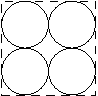
\includegraphics{Figures/four_circles}
\end{center}
%
Each particle touches a neighboring particle twice:
once within the core assembly and once again across a periodic
boundary.
\Dempla's underlying data structure allows for a single contact per
particle pair.
This problem is avoided with a larger number of particles.
\item
Do not try to control a boundary stress when the boundary stress
is zero.
For example, an input value \texttt{icontr=11100}
will not work with a diffuse, gaseous assembly
(\hyperref[sec:icontr]{Section~\ref*{sec:icontr}}).
\item\label{item:error2}
If you get an error message that your input files can not be properly read,
you will want to carefully check the formatting of the file's input
fields.
Microsoft Windows users may have problems with hidden characters that can
be embedded in files when using Word and Word Pad.
You will probably want to install a genuine text processor and
avoid using word processors.
%
\item\label{item:error10}
If at the start of a simulation you get the unexpected message,
``\texttt{Name of a platen file:}'', then you have probably given
\texttt{nplatn} a non-zero value in your 
\RunFile\ (see Section~\ref{sec:nplatn}).
%
\end{enumerate}
%
%
%
\section{Change Log}\label{sec:change_log}
This section documents the changes that have been made between various
version of \Oval\ and \Dempla.
%
%
%
\bibliographystyle{unsrtnat}
\bibliography{Kuhn}
%
%
\end{document}
